%%%%%%%%%%%%%%%%%%%%%%%%%%%%%%%%%%%%%%%%%%%%%%%%%%%%%%%%%%%%%%%
%
% Welcome to Overleaf --- just edit your article on the left,
% and we'll compile it for you on the right. If you give 
% someone the link to this page, they can edit at the same
% time. See the help menu above for more info. Enjoy!
%
%%%%%%%%%%%%%%%%%%%%%%%%%%%%%%%%%%%%%%%%%%%%%%%%%%%%%%%%%%%%%%%
%
% For more detailed article preparation guidelines, please see:
% http://f1000research.com/author-guidelines

\documentclass[10pt,a4paper,twocolumn]{article}
\usepackage{f1000_styles}

%% Default: numerical citations
\usepackage[numbers]{natbib}

%% Uncomment this lines for superscript citations instead
% \usepackage[super]{natbib}

%% Uncomment these lines for author-year citations instead
% \usepackage[round]{natbib}
% \let\cite\citep

\usepackage{hyperref}

\begin{document}

\title{\textit{F1000Research} Article Template}
\titlenote{The title should be detailed enough for someone to know whether the article would be of interest to them, but also concise. Please ensure the broadness and claims within the title are appropriate to the content of the article itself.}
\author[1,2]{Lisa M. Breckels}
\author[1,2]{Laurent Gatto}
\affil[1]{Computational Proteomics Unit, Cambridge Systems Biology Centre, University of Cambridge, Tennis Court Road, Cambridge, CB2 1GA, UK}
\affil[2]{Cambridge Centre for Proteomics, Department of Biochemistry, University of Cambridge, Tennis Court Road, Cambridge, CB2 1GA, UK}

\maketitle
\thispagestyle{fancy}


\begin{abstract}
Abstracts should be up to 300 words and provide a succinct summary of the article. Although the abstract should explain why the article might be interesting, care should be taken not to inappropriately over-emphasise the importance of the work described in the article. Citations should not be used in the abstract, and the use of abbreviations should be minimized. 
\end{abstract}

\clearpage




\section*{Introduction}

Quantitative mass spectrometry based spatial proteomics involves
elaborate, expensive and time consuming experimental procedures and
considerable effort is invested in the generation of such data.
Multiple research groups have described a variety of approaches to
establish high quality proteome-wide datasets (see for example
\cite{Gatto2010} for a review, and \cite{hyper,Itzhak:2016} for recent
examples). However, data analysis is as critical as data production
for reliable and insightful biological interpretation. Here, we walk
the reader through a typical pipeline for the analysis of such data
using several Bioconductor packages for the R statistical programming
environment.

The main package to analyse protein localisation data is
\Biocpkg{pRoloc}, which offers a set of dedicated functions for the
analysis of such data. \Biocpkg{pRoloc} itself relies on
\Biocpkg{MSnbase} to manipulate and process quantitative proteomics
data. Many other packages are used by \Biocpkg{pRoloc} for clustering,
classification and visualisation. Support for interactive
visualisation is offered by the \texttt{pRolocGUI} package.

In this workflow, we will describe how to prepare the spatial
proteomics data starting from a spreadsheet containing quantitative
mass spectrometry data, through to some essential data processing
steps, and finish with different applications of machine learning
(Figure \ref{fig:overview}). We focus on a recent pluripotent mouse
embryonic stem cells experiment \cite{hyper}. These data, as well as
additional annotated and pre-formatted datasets from various species
are readily available in the \Biocexptpkg{pRolocdata} package.

Installation of Bioconductor package is documented in detail on the
\href{http://bioconductor.org/install/#install-bioconductor-packages}{Bioconductor
  installation help page}. Below, we show how to install the four main
packages used in this workflow:

\begin{knitrout}
\definecolor{shadecolor}{rgb}{0.969, 0.969, 0.969}\color{fgcolor}\begin{kframe}
\begin{alltt}
\hlkwd{source}\hlstd{(}\hlstr{"https://bioconductor.org/biocLite.R"}\hlstd{)}
\hlkwd{biocLite}\hlstd{(}\hlkwd{c}\hlstd{(}\hlstr{"MSnase"}\hlstd{,} \hlstr{"pRoloc"}\hlstd{,} \hlstr{"pRolocdata"}\hlstd{,} \hlstr{"pRolocGUI"}\hlstd{))}
\end{alltt}
\end{kframe}
\end{knitrout}


This procedure is also applicable to any packages, from
\href{https://cran.r-project.org/}{CRAN} as well as GitHub. Once a
package has been installed, it needs to be loaded for its
functionality to become available in the R session; this is done with
the \texttt{library} function e.g.  to load the \Biocpkg{pRoloc} one
would type \texttt{library("pRoloc")} after installation.

If you have questions about this workflow in particular, or about
other Bioconductor packages in general, they are best asked on the
\href{https://support.bioconductor.org/}{Bioconductor support site}
following the
\href{http://www.bioconductor.org/help/support/posting-guide/}{posting
  guidelines}. Questions can be tagged with specific package names or
keywords. For more general information about mass spectrometry and
proteomics, the readers are invited to read the
\Biocexptpkg{RforProteomics} package vignettes and associated
papers \cite{Gatto:2014,Gatto:2015}.

\begin{figure}[!ht]
  \centering
  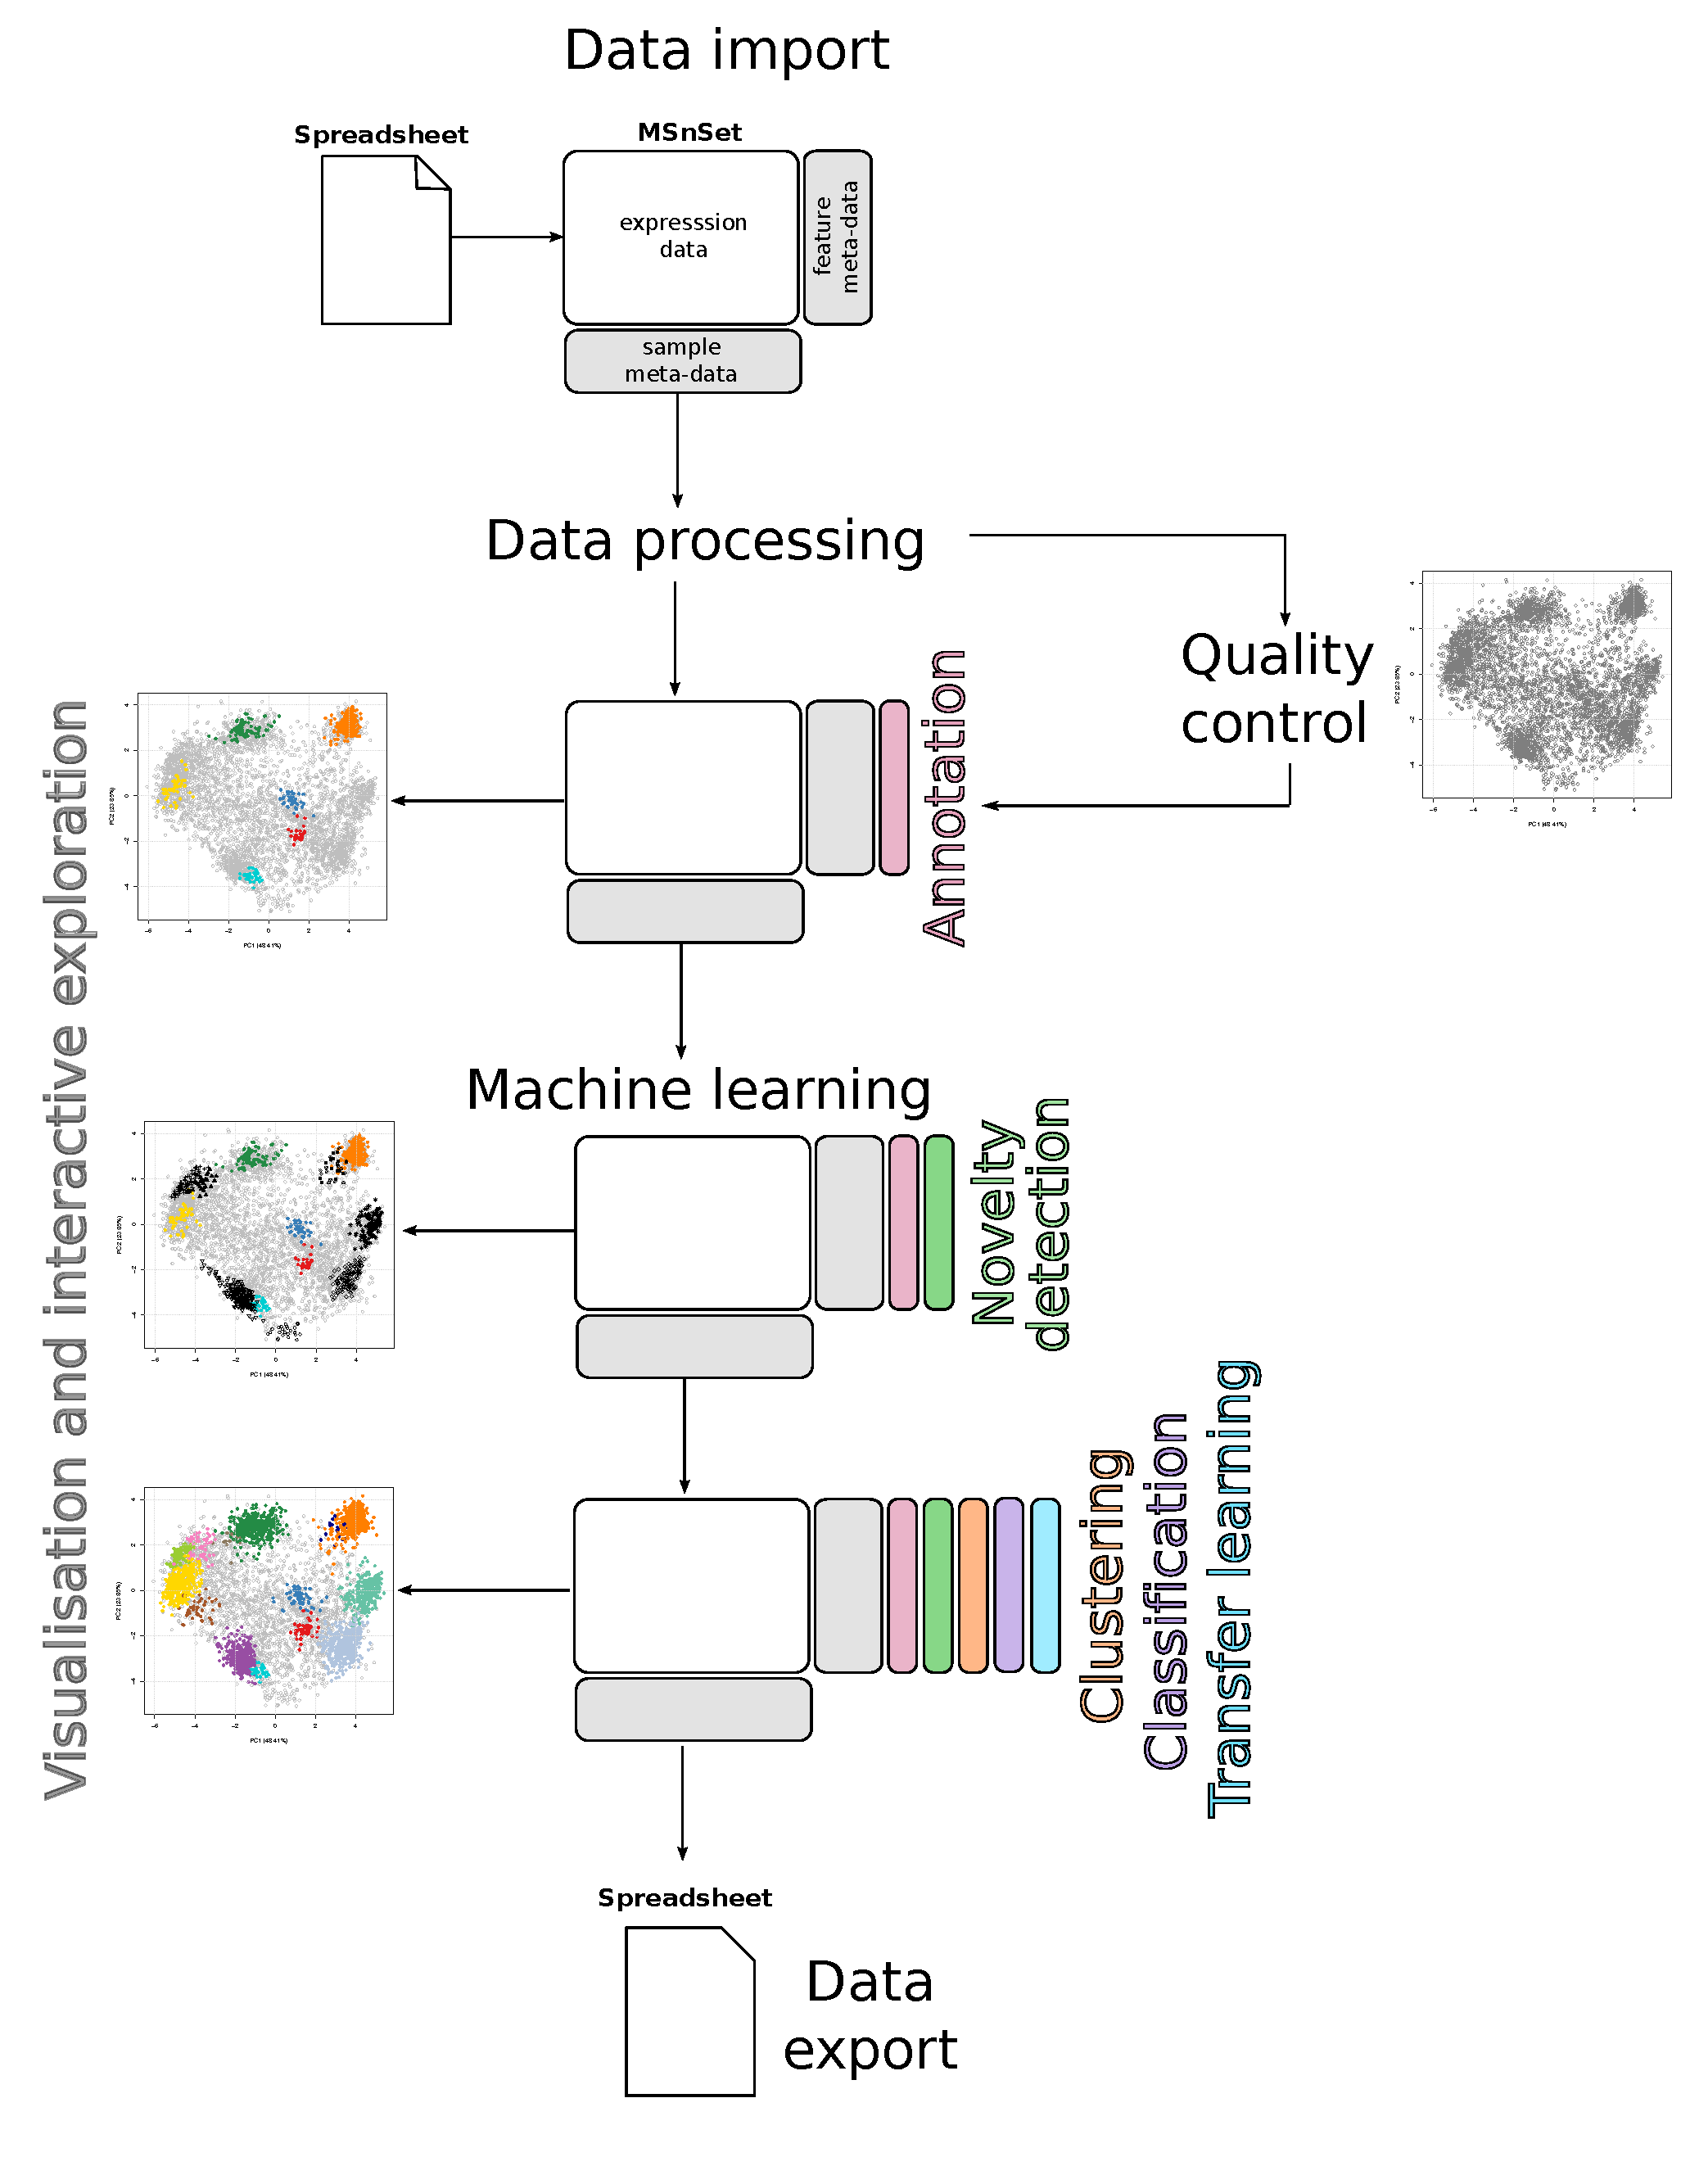
\includegraphics[width=.5\textwidth]{./Figures/overview.pdf}
  \caption{Schematic overview of the pRoloc pipeline from data import, through to data processing, machine learning and data export.}
  \label{fig:overview}
\end{figure}


\section*{Reading and processing spatial proteomics data}

\subsection*{The use-case: predicting sub-cellular localisation in pluripotent embryonic mouse stem cells}

As a use-case, we analyse a recent high-throughput spatial proteomics
dataset from pluripotent mouse embryonic stem cells (E14TG2a)
\cite{hyper}. The data was generated using hyperplexed LOPIT
(hyperLOPIT), a state-of-the-art method relying on improved
sub-cellular fractionation and more accurate quantitation, leading to
more reliable classification of protein localisation across the whole
sub-cellular space. The method uses an elaborate sub-cellular
fractionation scheme, enabled by the use of Tandem Mass Tag (TMT)
\cite{Thompson:2003} 10-plex and application of the MS data
acquisition technique named synchronous precursor selection MS$^3$
(SPS-MS$^3$) \cite{McAlister:2014}, for TMT quantification with high
accuracy and precision. Three biological replicates were generated
from the E14TG2a experiment, the first was to target low density
fractions and the second and third were to emphasis separation of the
denser organelles.  The intersect of replicates 1 and 2 was treated as
a 20-plex dataset for the analysis.  As discussed in the manuscript
\cite{hyper}, it has been shown that combining replicates from
different gradients can increase spatial resolution
\cite{Trotter:2010}. The combination of replicates resulted in 5032
proteins common in both experiments.

These, as well as many other data are directly available as properly
structured and annotated datasets from the \Biocexptpkg{pRolocdata}
experiment package. In this workflow, we will start with a description
of how to generate these ad hoc data objects starting from an
arbitrary spreadsheet, as produced by many popular third-party
applications.

While we focus here on a LOPIT-type dataset, these analyses are
relevant for any quantitative spatial proteomics data, irrespective of
the fractionation or quantitation (i.e. labelled or label-free)
methods.

\subsection*{The infrastructure: \texttt{pRoloc} and \texttt{MSnbase} packages}

To make use of the full functionality of the \Biocpkg{pRoloc} software
one needs to import their data into R and prepare them as an
\texttt{MSnSet}. The \texttt{MSnSet} is a dedicated data structure for
the efficient manipulation and processing of mass spectrometry and
proteomics data in R. Figure \ref{fig:msnset} illustrates a simplified view of the
\texttt{MSnSet} structure; there exists 3 key sub-parts (termed slots)
to such a data object: (1) the \texttt{exprs} (short for
\textit{expression} data) slot for storing the quantitation data, (2)
the \texttt{fData} slot (short for \textit{feature}-metadata) for
storing the feature meta-data, and finally (3) the \texttt{pData} slot
(short for \textit{pheno}-metadata, i.e. sample phenotypic data) for
storing the sample meta-data.

\begin{figure}[!ht]
  \centering
  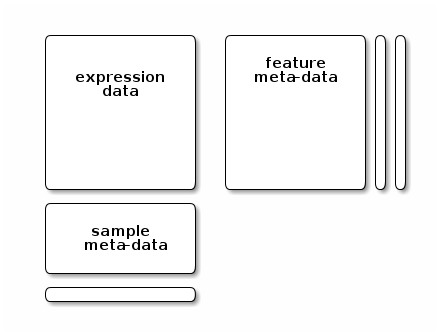
\includegraphics[width=.5\textwidth]{./Figures/msnset.png}
  \caption{Simplified representation of the \texttt{MSnSet} data
    structure (reproduced with permission from the \Biocpkg{MSnbase}
    vignette)}
  \label{fig:msnset}
\end{figure}

Feature metadata typically contains general annotation about the
proteins (accession numbers, description, \ldots), information related
to the identification search (confidence scores, number of peptides,
\ldots) as well as annotation about know sub-cellular location (see in
particular the \textit{Markers} section) and results from data
analysis. The sample metadata would, for example, record what
labelling ions were used for the respective fraction (when labelled
quantitation is used), replicate number, fraction number along the
gradient and pooling information.

Another slot of interest is \texttt{processingData}, that logs the
processing \texttt{MSnSet} objects undergo. The processing log can be
accessed with the \texttt{processingData} function and is displayed
under \textit{Processing information} in the textual object summary
when an \texttt{MSnSet}'s name it typed in the R console.

\subsection*{Importing data}

There are a number of ways to import quantitation data and create an
\texttt{MSnSet} instance. All methods are described in the
\Biocpkg{MSnbase}
\href{http://bioconductor.org/packages/release/bioc/vignettes/MSnbase/inst/doc/MSnbase-io.pdf}{input/output
  capabilities vignette}. One suggested simple method is to use the
function \texttt{readMSnSet2}. The function takes a single spreadsheet
file name as input and extracts the columns containing the
quantitation data, as identified by the argument \texttt{ecol}, to
create the expression data, while the other columns in the spreadsheet
are appended to the feature meta-data slot.  By example, in the code
chunk below we read in the \texttt{csv} spreadsheet containing the
quantitation data from the intersect of replicates 1 and 2 of the
mouse map \cite{hyper}, using the \texttt{readMSnSet2} function. The
data is as available online with the manuscript (see tab 2 of the
\texttt{xlsx} supplementary data set 1 in \cite{hyper}, which should
be exported as a text-based spreadsheet). It is also available as a
\texttt{csv} in the Bioconductor \Biocexptpkg{pRolocdata} data
package, which we make use of below.

To use the \texttt{readMSnSet2} function, as a minimum one must
specify the file path to the data and which columns of the spreadsheet
contain quantitation data. In the code chunk below, we start by
identifying the file that we want to use. The \texttt{system.file}
function is used to return the path to the \texttt{extdata} directory
from the \texttt{pRolocdata} package, which is where our file of
interest resides. We then use the \texttt{dir} function to list the
content of that directory and store the path that matches the file
name of interest in the \texttt{csvfile}. Note that these two lines
are only needed here to locate a file in a package; in a more general
use case, the user would defined the \texttt{csvfile} variable
containing the file name of interest directly.

A common pitfall here is to provide only the file name, rather than
full path to the file (which is what is shown below with
\texttt{basename}; we don't print the full path, as it will vary from
computer to computer). Note that only specifying the name of the file
is sufficient when it exists in the working directory (i.e. the
directory in which R is running, which can be queried and changed with
the \texttt{getwd} and \texttt{setwd} functions respectively).

\begin{knitrout}
\definecolor{shadecolor}{rgb}{0.969, 0.969, 0.969}\color{fgcolor}\begin{kframe}
\begin{alltt}
\hlkwd{library}\hlstd{(}\hlstr{"MSnbase"}\hlstd{)}
\hlstd{extdatadir} \hlkwb{<-} \hlkwd{system.file}\hlstd{(}\hlstr{"extdata"}\hlstd{,} \hlkwc{package} \hlstd{=} \hlstr{"pRolocdata"}\hlstd{)}
\hlstd{csvfile} \hlkwb{<-} \hlkwd{dir}\hlstd{(extdatadir,} \hlkwc{full.names} \hlstd{=} \hlnum{TRUE}\hlstd{,}
          \hlkwc{pattern} \hlstd{=} \hlstr{"hyperLOPIT-SIData-ms3-rep12-intersect.csv"}\hlstd{)}
\hlkwd{basename}\hlstd{(csvfile)}
\end{alltt}
\begin{verbatim}
## [1] "hyperLOPIT-SIData-ms3-rep12-intersect.csv.gz"
\end{verbatim}
\end{kframe}
\end{knitrout}

Note that the file is compressed (as indicated by the \texttt{gz}, for
\texttt{gzip}, extension), and will be decompressed on-the-fly when
read into R.

Next, we need to identify which columns in the spreadsheet contain the
quantitation data. This can be done using the \texttt{getEcols}
function inside R. The spreadsheet that was deposited by the authors
contains two headers, with the second header containing information
about where the quantitation data is stored.

\begin{figure}[!ht]
  \centering
  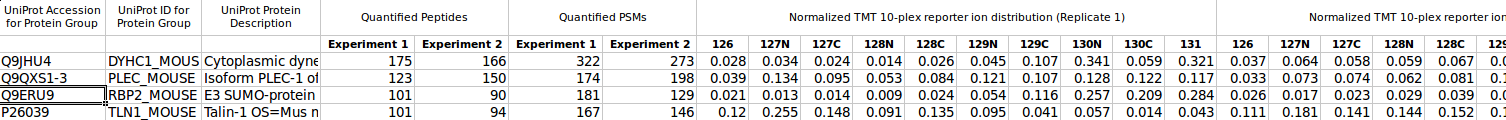
\includegraphics[width=.85\textwidth]{./Figures/spreadsheet-screenshot.png}
  \caption{A screenshot of the data in the spreadsheet.}
  \label{fig:spreadsheet}
\end{figure}


We can display the names of the second header by calling the
\texttt{getEcols} function with the argument \texttt{n = 2} (the
default value is \texttt{n = 1}), to specify that we wish to display
the column names of the second line. We also specify the name of the
spreadsheet file (defined as \texttt{csvfile} above) and the
separator that splits cells.

\begin{knitrout}
\definecolor{shadecolor}{rgb}{0.969, 0.969, 0.969}\color{fgcolor}\begin{kframe}
\begin{alltt}
\hlkwd{getEcols}\hlstd{(csvfile,} \hlkwc{split} \hlstd{=} \hlstr{","}\hlstd{,} \hlkwc{n} \hlstd{=} \hlnum{2}\hlstd{)}
\end{alltt}
\begin{verbatim}
##  [1] ""                                 
##  [2] ""                                 
##  [3] ""                                 
##  [4] "Experiment 1"                     
##  [5] "Experiment 2"                     
##  [6] "Experiment 1"                     
##  [7] "Experiment 2"                     
##  [8] "126"                              
##  [9] "127N"                             
## [10] "127C"                             
## [11] "128N"                             
## [12] "128C"                             
## [13] "129N"                             
## [14] "129C"                             
## [15] "130N"                             
## [16] "130C"                             
## [17] "131"                              
## [18] "126"                              
## [19] "127N"                             
## [20] "127C"                             
## [21] "128N"                             
## [22] "128C"                             
## [23] "129N"                             
## [24] "129C"                             
## [25] "130N"                             
## [26] "130C"                             
## [27] "131"                              
## [28] "phenoDisco Input"                 
## [29] "phenoDisco Output"                
## [30] "Curated phenoDisco Output"        
## [31] "SVM marker set"                   
## [32] "SVM classification"               
## [33] "SVM score"                        
## [34] "SVM classification (top quartile)"
## [35] "Final Localization Assignment"    
## [36] "First localization evidence?"     
## [37] "Curated Organelles"               
## [38] "Cytoskeletal Components"          
## [39] "Trafficking Proteins"             
## [40] "Protein Complexes"                
## [41] "Signaling Cascades"               
## [42] "Oct4 Interactome"                 
## [43] "Nanog Interactome"                
## [44] "Sox2 Interactome"                 
## [45] "Cell Surface Proteins"
\end{verbatim}
\end{kframe}
\end{knitrout}

It is now easy for one to identify that the quantitation data,
corresponding to the 10 TMT isobaric tags, is located in columns 8
to 27. We now have the two mandatory arguments to \texttt{readMSnSet2},
namely the file name (stored in the \texttt{csvfile} variable) and the
quantitation column indices. In addition to these, it is also possible
to pass the optional argument \texttt{fnames} to indicate which column to use
as the labels by which to identify each protein in the sample. Here,
we use \texttt{fnames = 1} to use the UniProt identifiers contained in the
first (unnamed) column of the spreadsheet. We also need to specify to
skip the first line of the file (for the same reason that we used 
\texttt{n = 2} in \texttt{getEcols} above) to read the \texttt{csv} data and convert it to an
\texttt{MSnSet} object, named \texttt{hl} (for hyperLOPIT).

\begin{knitrout}
\definecolor{shadecolor}{rgb}{0.969, 0.969, 0.969}\color{fgcolor}\begin{kframe}
\begin{alltt}
\hlstd{hl} \hlkwb{<-} \hlkwd{readMSnSet2}\hlstd{(csvfile,} \hlkwc{ecol} \hlstd{=} \hlnum{8}\hlopt{:}\hlnum{27}\hlstd{,} \hlkwc{fnames} \hlstd{=} \hlnum{1}\hlstd{,} \hlkwc{skip} \hlstd{=} \hlnum{1}\hlstd{)}
\end{alltt}
\end{kframe}
\end{knitrout}

Below, we display a short summary of the data. The data contains 
5032 proteins/features common across the 2 biological replicates
for the respective 2 x 10-plex reporter tags (20
columns/samples), along with associated feature meta-data such as
protein markers, protein description, number of quantified peptides
etc (see below).


\begin{knitrout}
\definecolor{shadecolor}{rgb}{0.969, 0.969, 0.969}\color{fgcolor}\begin{kframe}
\begin{alltt}
\hlstd{hl}
\end{alltt}
\begin{verbatim}
## MSnSet (storageMode: lockedEnvironment)
## assayData: 5032 features, 20 samples 
##   element names: exprs 
## protocolData: none
## phenoData: none
## featureData
##   featureNames: Q9JHU4 Q9QXS1-3 ... Q9Z2R6 (5032 total)
##   fvarLabels: X X.1 ... Cell.Surface.Proteins (25 total)
##   fvarMetadata: labelDescription
## experimentData: use 'experimentData(object)'
## Annotation:  
## - - - Processing information - - -
##  MSnbase version: 2.1.4
\end{verbatim}
\end{kframe}
\end{knitrout}

Below, we examine the quantitative information along the whole
gradient for first 5 proteins.  It is also possible to access specific
rows and columns by naming the proteins and TMT tag channels of
interest.

\begin{knitrout}
\definecolor{shadecolor}{rgb}{0.969, 0.969, 0.969}\color{fgcolor}\begin{kframe}
\begin{alltt}
\hlkwd{exprs}\hlstd{(hl)[}\hlnum{1}\hlopt{:}\hlnum{5}\hlstd{, ]}
\end{alltt}
\begin{verbatim}
##           X126 X127N X127C X128N X128C X129N X129C X130N X130C  X131
## Q9JHU4   0.028 0.034 0.024 0.014 0.026 0.045 0.107 0.341 0.059 0.321
## Q9QXS1-3 0.039 0.134 0.095 0.053 0.084 0.121 0.107 0.128 0.122 0.117
## Q9ERU9   0.021 0.013 0.014 0.009 0.024 0.054 0.116 0.257 0.209 0.284
## P26039   0.120 0.255 0.148 0.091 0.135 0.095 0.041 0.057 0.014 0.043
## Q8BTM8   0.055 0.139 0.078 0.050 0.077 0.098 0.093 0.171 0.079 0.160
##          X126.1 X127N.1 X127C.1 X128N.1 X128C.1 X129N.1 X129C.1 X130N.1
## Q9JHU4    0.037   0.064   0.058   0.059   0.067   0.078   0.140   0.208
## Q9QXS1-3  0.033   0.073   0.074   0.062   0.081   0.142   0.190   0.069
## Q9ERU9    0.026   0.017   0.023   0.029   0.039   0.071   0.105   0.171
## P26039    0.111   0.181   0.141   0.144   0.152   0.119   0.075   0.028
## Q8BTM8    0.062   0.108   0.091   0.086   0.099   0.111   0.117   0.095
##          X130C.1 X131.1
## Q9JHU4     0.141  0.147
## Q9QXS1-3   0.151  0.125
## Q9ERU9     0.304  0.215
## P26039     0.017  0.033
## Q8BTM8     0.144  0.087
\end{verbatim}
\begin{alltt}
\hlkwd{exprs}\hlstd{(hl)[}\hlkwd{c}\hlstd{(}\hlstr{"Q9ERU9"}\hlstd{,} \hlstr{"Q9Z2R6"}\hlstd{),} \hlkwd{c}\hlstd{(}\hlstr{"X126"}\hlstd{,} \hlstr{"X131.1"}\hlstd{)]}
\end{alltt}
\begin{verbatim}
##         X126 X131.1
## Q9ERU9 0.021  0.215
## Q9Z2R6 0.563  0.000
\end{verbatim}
\end{kframe}
\end{knitrout}

The feature meta-data is stored in the \texttt{fData} slot and can be
accessed by \texttt{fData(hl)}. When using \texttt{readMSnSet2}, automatically,
everything that is not defined as quantitation data by \texttt{ecol} or the
feature names by \texttt{fnames} is deposited to the \texttt{fData} slot. 

We see the \texttt{fData} contains 25 columns describing information such as
the number of peptides, associated markers, machine learning results
etc. To identify the feature variable names we can use the function
\texttt{fvarLabels}. We see that the first 6 feature variable names contain
non-discriminatory label names, so we relabel them to help us identify
what feature data information is stored in the associated columns.

\begin{knitrout}
\definecolor{shadecolor}{rgb}{0.969, 0.969, 0.969}\color{fgcolor}\begin{kframe}
\begin{alltt}
\hlkwd{fvarLabels}\hlstd{(hl)}
\end{alltt}
\begin{verbatim}
##  [1] "X"                                
##  [2] "X.1"                              
##  [3] "X.2"                              
##  [4] "Experiment.1"                     
##  [5] "Experiment.2"                     
##  [6] "Experiment.1.1"                   
##  [7] "Experiment.2.1"                   
##  [8] "phenoDisco.Input"                 
##  [9] "phenoDisco.Output"                
## [10] "Curated.phenoDisco.Output"        
## [11] "SVM.marker.set"                   
## [12] "SVM.classification"               
## [13] "SVM.score"                        
## [14] "SVM.classification..top.quartile."
## [15] "Final.Localization.Assignment"    
## [16] "First.localization.evidence."     
## [17] "Curated.Organelles"               
## [18] "Cytoskeletal.Components"          
## [19] "Trafficking.Proteins"             
## [20] "Protein.Complexes"                
## [21] "Signaling.Cascades"               
## [22] "Oct4.Interactome"                 
## [23] "Nanog.Interactome"                
## [24] "Sox2.Interactome"                 
## [25] "Cell.Surface.Proteins"
\end{verbatim}
\begin{alltt}
\hlkwd{fvarLabels}\hlstd{(hl)[}\hlnum{1}\hlopt{:}\hlnum{3}\hlstd{]} \hlkwb{<-} \hlkwd{c}\hlstd{(}\hlstr{"uniprot.accession"}\hlstd{,} \hlstr{"uniprot.id"}\hlstd{,} \hlstr{"description"}\hlstd{)}
\hlkwd{fvarLabels}\hlstd{(hl)[}\hlnum{4}\hlopt{:}\hlnum{6}\hlstd{]} \hlkwb{<-} \hlkwd{paste0}\hlstd{(}\hlstr{"peptides.expt"}\hlstd{,} \hlnum{1}\hlopt{:}\hlnum{3}\hlstd{)}
\hlcom{## feature vars 1, 2, and 4 to 6}
\hlkwd{fData}\hlstd{(hl)[}\hlnum{1}\hlopt{:}\hlnum{4}\hlstd{,} \hlkwd{c}\hlstd{(}\hlnum{1}\hlopt{:}\hlnum{2}\hlstd{,} \hlnum{4}\hlopt{:}\hlnum{6}\hlstd{)]}
\end{alltt}
\begin{verbatim}
##          uniprot.accession  uniprot.id peptides.expt1 peptides.expt2
## Q9JHU4              Q9JHU4 DYHC1_MOUSE            175            166
## Q9QXS1-3          Q9QXS1-3  PLEC_MOUSE            123            150
## Q9ERU9              Q9ERU9  RBP2_MOUSE            101             90
## P26039              P26039  TLN1_MOUSE            101             94
##          peptides.expt3
## Q9JHU4              322
## Q9QXS1-3            174
## Q9ERU9              181
## P26039              167
\end{verbatim}
\end{kframe}
\end{knitrout}

Note that when using the simple \texttt{readMSnSet2} procedure, the
\texttt{pData} slot which is used to store information about the
samples/channels is kept empty. As illustrated below, one can use the
\texttt{\$} operator to access (or create) individual columns in the
metadata slot. It is advised to annotate the channels as well. Below,
we annotate the replicate from which the profiles originate and the
TMT tag (extracted from the sample/channel names). To do so, we use
the sample names that were assigned automatically using the
quantiation column names and remove leading \texttt{X} and trailing
\texttt{.1} using the \texttt{sub} function.

\begin{knitrout}
\definecolor{shadecolor}{rgb}{0.969, 0.969, 0.969}\color{fgcolor}\begin{kframe}
\begin{alltt}
\hlkwd{pData}\hlstd{(hl)}\hlopt{$}\hlstd{Replicate} \hlkwb{<-} \hlkwd{rep}\hlstd{(}\hlnum{1}\hlopt{:}\hlnum{2}\hlstd{,} \hlkwc{each} \hlstd{=} \hlnum{10}\hlstd{)}
\hlkwd{pData}\hlstd{(hl)}\hlopt{$}\hlstd{Tag} \hlkwb{<-} \hlkwd{sub}\hlstd{(}\hlstr{"\textbackslash{}\textbackslash{}.1$"}\hlstd{,} \hlstr{""}\hlstd{,} \hlkwd{sub}\hlstd{(}\hlstr{"^X"}\hlstd{,} \hlstr{""}\hlstd{,} \hlkwd{sampleNames}\hlstd{(hl)))}
\hlkwd{pData}\hlstd{(hl)}
\end{alltt}
\begin{verbatim}
##         Replicate  Tag
## X126            1  126
## X127N           1 127N
## X127C           1 127C
## X128N           1 128N
## X128C           1 128C
## X129N           1 129N
## X129C           1 129C
## X130N           1 130N
## X130C           1 130C
## X131            1  131
## X126.1          2  126
## X127N.1         2 127N
## X127C.1         2 127C
## X128N.1         2 128N
## X128C.1         2 128C
## X129N.1         2 129N
## X129C.1         2 129C
## X130N.1         2 130N
## X130C.1         2 130C
## X131.1          2  131
\end{verbatim}
\end{kframe}
\end{knitrout}

Throughout this workflow we refer to the different columns that
are found in the \texttt{exprs} (expression data) slot as channels (short for TMT channels).
In the frame of LOPIT and hyperLOPIT these channels constitute the
relative abundance of each protein (along the rows) in the channel of
interest. Each TMT channel originates from fractions collected from
the density gradient, or a set of pooled fractions or may be a sample
originating from an alternative preparation e.g. such as from the
chromatin enrichment performed in Christoforou et al \cite{hyper}.
Information about which gradient fractions were used for which tag
should also be stored in the sample meta-data \texttt{pData} slot.

The sample meta-data that is distributed with the
\Biocexptpkg{pRolocdata} package for Christoforou's
hyperLOPIT experiment and (as above) the quantitation data file, are
located in the \texttt{extdata} in the \Biocexptpkg{pRolocdata}
package on the hard drive.

In the code chunk below we again use the
\texttt{dir} function to locate the filepath to the meta-data \texttt{csv} file and
then read it into R using \texttt{read.csv}. We then append the meta-data to
the \texttt{pData} slot.  Information about the gradient fractions used and
the associated subcellular fraction densities in % w/v Iodixanol for
each replicate are stored here.

\begin{knitrout}
\definecolor{shadecolor}{rgb}{0.969, 0.969, 0.969}\color{fgcolor}\begin{kframe}
\begin{alltt}
\hlstd{expinfo} \hlkwb{<-} \hlkwd{dir}\hlstd{(extdatadir,} \hlkwc{full.names} \hlstd{=} \hlnum{TRUE}\hlstd{,}
               \hlkwc{pattern} \hlstd{=} \hlstr{"hyperLOPIT-SIData-fraction-info.csv"}\hlstd{)}

\hlstd{fracinfo} \hlkwb{<-} \hlkwd{read.csv}\hlstd{(expinfo,} \hlkwc{row.names}\hlstd{=}\hlnum{1}\hlstd{,} \hlkwc{skip} \hlstd{=} \hlnum{2}\hlstd{,}
                     \hlkwc{header} \hlstd{=} \hlnum{FALSE}\hlstd{,} \hlkwc{stringsAsFactors} \hlstd{=} \hlnum{FALSE}\hlstd{)}

\hlkwd{pData}\hlstd{(hl)}\hlopt{$}\hlstd{Gradient.Fraction} \hlkwb{<-} \hlkwd{c}\hlstd{(fracinfo[,} \hlnum{1}\hlstd{], fracinfo[,} \hlnum{2}\hlstd{])}
\hlkwd{pData}\hlstd{(hl)}\hlopt{$}\hlstd{Iodixonal.Density} \hlkwb{<-} \hlkwd{c}\hlstd{(fracinfo[,} \hlnum{4}\hlstd{], fracinfo[,} \hlnum{5}\hlstd{])}
\hlkwd{pData}\hlstd{(hl)}
\end{alltt}
\begin{verbatim}
##         Replicate  Tag Gradient.Fraction Iodixonal.Density
## X126            1  126           Cytosol               0.0
## X127N           1 127N   1 to 6 (pooled)               6.0
## X127C           1 127C   8 to 9 (pooled)              11.0
## X128N           1 128N 10 to 11 (pooled)              13.3
## X128C           1 128C                12              14.6
## X129N           1 129N                14              17.4
## X129C           1 129C                16              20.1
## X130N           1 130N                18              26.8
## X130C           1 130C         Chromatin                NA
## X131            1  131                19              34.5
## X126.1          2  126           Cytosol               0.0
## X127N.1         2 127N   1 to 6 (pooled)               5.2
## X127C.1         2 127C   7 to 9 (pooled)              10.0
## X128N.1         2 128N 10 to 11 (pooled)              12.5
## X128C.1         2 128C                12              14.0
## X129N.1         2 129N 14 to 15 (pooled)              17.3
## X129C.1         2 129C                17              20.9
## X130N.1         2 130N 18 to 19 (pooled)              24.7
## X130C.1         2 130C         Chromatin                NA
## X131.1          2  131                20              31.9
\end{verbatim}
\end{kframe}
\end{knitrout}

\subsection*{Data processing}

\subsubsection*{Normalisation}

There are two aspects related to data normalisation that are relevant
to spatial proteomics data processing. The first one focuses on
reducing purely technical variation between channels without affecting
biological variability (i.e. the shape of the quantitative
profiles). This normalisation will depend on the underlying
quantitative technology and the experimental design, and will not be
addressed in this workflow. The second aspect, and more specific to
spatial proteomics data, is scaling all the organelle-specific
profiles into a same intensity interval (typically 0 and 1) by, for
example, dividing each intensity by the sum of the intensities for
that quantitative feature. This is not necessary in this example as
the intensities for each replicate have already been re-scaled to 1 in
Proteome Discoverer v1.4, Thermo Fisher. However, if one wanted to do
this they would execute the \texttt{normalise} function as
demonstrated in the below code chunk.

\begin{knitrout}
\definecolor{shadecolor}{rgb}{0.969, 0.969, 0.969}\color{fgcolor}\begin{kframe}
\begin{alltt}
\hlstd{hl} \hlkwb{<-} \hlkwd{normalise}\hlstd{(hl,} \hlkwc{method} \hlstd{=} \hlstr{"sum"}\hlstd{)}
\end{alltt}
\end{kframe}
\end{knitrout}

This transformation of the data assures to cancel the effect of the
absolute intensities of the quantitative features along the rows, to
focus subsequent analyses on the relative profiles along the
sub-cellular channels.

The same \texttt{normalise} function (or \texttt{normalize}, both
spellings are supported) can also be applied in the first case
described above.  Different normalisation methods, such as mean or
median scaling, variance stabilisation or quantile normalisation, to
cite a few, can be applied to accomodate different needs (see
\texttt{?normalise} for available options).

As previously mentioned, before combination, the two replicates in the
\texttt{hl} data that we read into R were separately normalised by sum (i.e.
to 1) across the 10 channels for each replicate respectively. We can
verify this by summing each rows for each replicate:

\begin{knitrout}
\definecolor{shadecolor}{rgb}{0.969, 0.969, 0.969}\color{fgcolor}\begin{kframe}
\begin{alltt}
\hlkwd{summary}\hlstd{(}\hlkwd{rowSums}\hlstd{(}\hlkwd{exprs}\hlstd{(hl[, hl}\hlopt{$}\hlstd{Replicate} \hlopt{==} \hlnum{1}\hlstd{])))}
\end{alltt}
\begin{verbatim}
##    Min. 1st Qu.  Median    Mean 3rd Qu.    Max. 
##   0.997   0.999   1.000   1.000   1.001   1.003
\end{verbatim}
\begin{alltt}
\hlkwd{summary}\hlstd{(}\hlkwd{rowSums}\hlstd{(}\hlkwd{exprs}\hlstd{(hl[, hl}\hlopt{$}\hlstd{Replicate} \hlopt{==} \hlnum{2}\hlstd{])))}
\end{alltt}
\begin{verbatim}
##    Min. 1st Qu.  Median    Mean 3rd Qu.    Max. 
##   0.997   0.999   1.000   1.000   1.001   1.003
\end{verbatim}
\end{kframe}
\end{knitrout}

We see that some features do not add up exactly to 1 due to rounding
errors after exporting to intermediate files. These small deviations
do not bear any consequences here.


\subsubsection*{Combining acquisitions}

The spreadsheet that was used to create the \texttt{hl}
\texttt{MSnSet} included the two replicates within one .csv file.  We
also provide individual replicates in the \Biocexptpkg{pRolocdata}
package. Below, we show how to combine \texttt{MSnSet} objects and,
subsequently, how to filter and handle missing values. We start by
loading the \Biocexptpkg{pRolocdata} package and the equivalent
replicates using the \texttt{data} function.

\begin{knitrout}
\definecolor{shadecolor}{rgb}{0.969, 0.969, 0.969}\color{fgcolor}\begin{kframe}
\begin{alltt}
\hlkwd{library}\hlstd{(}\hlstr{"pRolocdata"}\hlstd{)}
\hlkwd{data}\hlstd{(hyperLOPIT2015ms3r1)}
\hlkwd{data}\hlstd{(hyperLOPIT2015ms3r2)}
\end{alltt}
\end{kframe}
\end{knitrout}

At the R prompt, typing

\begin{knitrout}
\definecolor{shadecolor}{rgb}{0.969, 0.969, 0.969}\color{fgcolor}\begin{kframe}
\begin{alltt}
\hlkwd{pRolocdata}\hlstd{()}
\end{alltt}
\end{kframe}
\end{knitrout}

will list the 54 datasets that are
available in \Biocexptpkg{pRolocdata}.

%% $

Combining data is performed with the \texttt{combine} function. This
function will inspect the feature and sample names to identify how to
combine the data. As we want our replicates to be combined along the
columns (same proteins, different sets of channels), we need to assure
that the respective sample names differ so they can be identified from
one another. The function \texttt{updateSampleNames} can be used do
this.

\begin{knitrout}
\definecolor{shadecolor}{rgb}{0.969, 0.969, 0.969}\color{fgcolor}\begin{kframe}
\begin{alltt}
\hlkwd{identical}\hlstd{(}\hlkwd{sampleNames}\hlstd{(hyperLOPIT2015ms3r1),} \hlkwd{sampleNames}\hlstd{(hyperLOPIT2015ms3r2))}
\end{alltt}
\begin{verbatim}
## [1] TRUE
\end{verbatim}
\begin{alltt}
\hlstd{hyperLOPIT2015ms3r1} \hlkwb{<-} \hlkwd{updateSampleNames}\hlstd{(hyperLOPIT2015ms3r1,} \hlnum{1}\hlstd{)}
\hlstd{hyperLOPIT2015ms3r2} \hlkwb{<-} \hlkwd{updateSampleNames}\hlstd{(hyperLOPIT2015ms3r2,} \hlnum{2}\hlstd{)}
\hlkwd{sampleNames}\hlstd{(hyperLOPIT2015ms3r1)}
\end{alltt}
\begin{verbatim}
##  [1] "X126.1"  "X127N.1" "X127C.1" "X128N.1" "X128C.1" "X129N.1" "X129C.1"
##  [8] "X130N.1" "X130C.1" "X131.1"
\end{verbatim}
\begin{alltt}
\hlkwd{sampleNames}\hlstd{(hyperLOPIT2015ms3r2)}
\end{alltt}
\begin{verbatim}
##  [1] "X126.2"  "X127N.2" "X127C.2" "X128N.2" "X128C.2" "X129N.2" "X129C.2"
##  [8] "X130N.2" "X130C.2" "X131.2"
\end{verbatim}
\end{kframe}
\end{knitrout}

In addition to matching names, the content of the feature metadata for
identical feature annotations must match exactly across the data to be
combined. In particular for these data, we expect the same proteins in
each replicate to be annotated with the same UniProt entry names and
descriptions, but not with the same coverage of number of peptides or
peptide-spectrum matches (PSMs).

\begin{knitrout}
\definecolor{shadecolor}{rgb}{0.969, 0.969, 0.969}\color{fgcolor}\begin{kframe}
\begin{alltt}
\hlkwd{fvarLabels}\hlstd{(hyperLOPIT2015ms3r1)}
\end{alltt}
\begin{verbatim}
## [1] "EntryName"          "ProteinDescription" "Peptides"          
## [4] "PSMs"               "ProteinCoverage"    "markers"
\end{verbatim}
\begin{alltt}
\hlkwd{fvarLabels}\hlstd{(hyperLOPIT2015ms3r2)}
\end{alltt}
\begin{verbatim}
## [1] "EntryName"          "ProteinDescription" "Peptides"          
## [4] "PSMs"               "ProteinCoverage"    "markers"
\end{verbatim}
\end{kframe}
\end{knitrout}

Below, we update the replicate specific feature variable names and
remove the shared annotation. In the first line, we update only the
feature variable names 3 to 5 (by appending a \texttt{1}) and in the
second line, we apply the \texttt{updateFvarLabels} function to update
all feature variable names (by appending a \texttt{2}).

\begin{knitrout}
\definecolor{shadecolor}{rgb}{0.969, 0.969, 0.969}\color{fgcolor}\begin{kframe}
\begin{alltt}
\hlkwd{fvarLabels}\hlstd{(hyperLOPIT2015ms3r1)[}\hlnum{3}\hlopt{:}\hlnum{5}\hlstd{]} \hlkwb{<-} \hlkwd{paste0}\hlstd{(}\hlkwd{fvarLabels}\hlstd{(hyperLOPIT2015ms3r1)[}\hlnum{3}\hlopt{:}\hlnum{5}\hlstd{],} \hlnum{1}\hlstd{)}
\hlstd{hyperLOPIT2015ms3r2} \hlkwb{<-} \hlkwd{updateFvarLabels}\hlstd{(hyperLOPIT2015ms3r2,} \hlstr{"2"}\hlstd{,} \hlkwc{sep} \hlstd{=} \hlstr{""}\hlstd{)}
\hlkwd{fData}\hlstd{(hyperLOPIT2015ms3r1)} \hlkwb{<-} \hlkwd{fData}\hlstd{(hyperLOPIT2015ms3r1)[}\hlnum{1}\hlopt{:}\hlnum{5}\hlstd{]}
\hlkwd{fData}\hlstd{(hyperLOPIT2015ms3r2)} \hlkwb{<-} \hlkwd{fData}\hlstd{(hyperLOPIT2015ms3r2)[}\hlnum{3}\hlopt{:}\hlnum{5}\hlstd{]}
\hlkwd{fvarLabels}\hlstd{(hyperLOPIT2015ms3r1)}
\end{alltt}
\begin{verbatim}
## [1] "EntryName"          "ProteinDescription" "Peptides1"         
## [4] "PSMs1"              "ProteinCoverage1"
\end{verbatim}
\begin{alltt}
\hlkwd{fvarLabels}\hlstd{(hyperLOPIT2015ms3r2)}
\end{alltt}
\begin{verbatim}
## [1] "Peptides2"        "PSMs2"            "ProteinCoverage2"
\end{verbatim}
\end{kframe}
\end{knitrout}

We can now combine the two experiments into a single \texttt{MSnSet}:

\begin{knitrout}
\definecolor{shadecolor}{rgb}{0.969, 0.969, 0.969}\color{fgcolor}\begin{kframe}
\begin{alltt}
\hlstd{combined} \hlkwb{<-} \hlkwd{combine}\hlstd{(hyperLOPIT2015ms3r1, hyperLOPIT2015ms3r2)}
\hlstd{combined}
\end{alltt}
\begin{verbatim}
## MSnSet (storageMode: lockedEnvironment)
## assayData: 6725 features, 20 samples 
##   element names: exprs 
## protocolData: none
## phenoData
##   sampleNames: X126.1 X127N.1 ... X131.2 (20 total)
##   varLabels: Replicate TMT.Reagent ... Iodixonal.Density (5 total)
##   varMetadata: labelDescription
## featureData
##   featureNames: Q9JHU4 Q9QXS1-3 ... Q9Z2Y3-3 (6725 total)
##   fvarLabels: EntryName ProteinDescription ... ProteinCoverage2 (8
##     total)
##   fvarMetadata: labelDescription
## experimentData: use 'experimentData(object)'
## Annotation:  
## - - - Processing information - - -
## Combined [6725,20] and [6268,10] MSnSets Fri Dec  2 17:19:06 2016 
##  MSnbase version: 1.21.7
\end{verbatim}
\end{kframe}
\end{knitrout}

More details about combining data are given in the dedicated
\textit{Combining MSnSet instances} section of the \Biocpkg{MSnbase}
\href{http://bioconductor.org/packages/release/bioc/vignettes/MSnbase/inst/doc/MSnbase-demo.pdf}{tutorial
  vignette}.

\subsubsection*{Missing data}

Missing data are a recurrent issue in mass spectrometry applications,
and should be addressed independently of this workflow
\cite{Webb-Robertson:2015,Lazar:2016}. In \cite{Gatto:2014b}, we have
described how a high content in missing values in spatial proteomics
data and their inappropriate handling leads to a reduction of
sub-cellular resolution. Missing data can be imputated using
\Biocpkg{MSnbase}'s \texttt{impute} function. The method underlying
the imputation method is then determined by a \texttt{methods}
parameter. To impute missing values using nearest neighbour
imputation, one would

\begin{knitrout}
\definecolor{shadecolor}{rgb}{0.969, 0.969, 0.969}\color{fgcolor}\begin{kframe}
\begin{alltt}
\hlstd{hl} \hlkwb{<-} \hlkwd{impute}\hlstd{(hl,} \hlkwc{method} \hlstd{=} \hlstr{"knn"}\hlstd{)}
\end{alltt}
\end{kframe}
\end{knitrout}

In our particular case, missing values are indicative of protein
groups that were not acquired in both replicates (Figure
\ref{fig:namap}).

\begin{figure}[!ht]
  \centering
\begin{knitrout}
\definecolor{shadecolor}{rgb}{0.969, 0.969, 0.969}\color{fgcolor}\begin{kframe}
\begin{alltt}
\hlkwd{image2}\hlstd{(}\hlkwd{is.na}\hlstd{(combined),} \hlkwc{col} \hlstd{=} \hlkwd{c}\hlstd{(}\hlstr{"black"}\hlstd{,} \hlstr{"white"}\hlstd{),}
       \hlkwc{main} \hlstd{=} \hlstr{"Missing values (white cells) after combining replicates"}\hlstd{)}
\end{alltt}
\end{kframe}
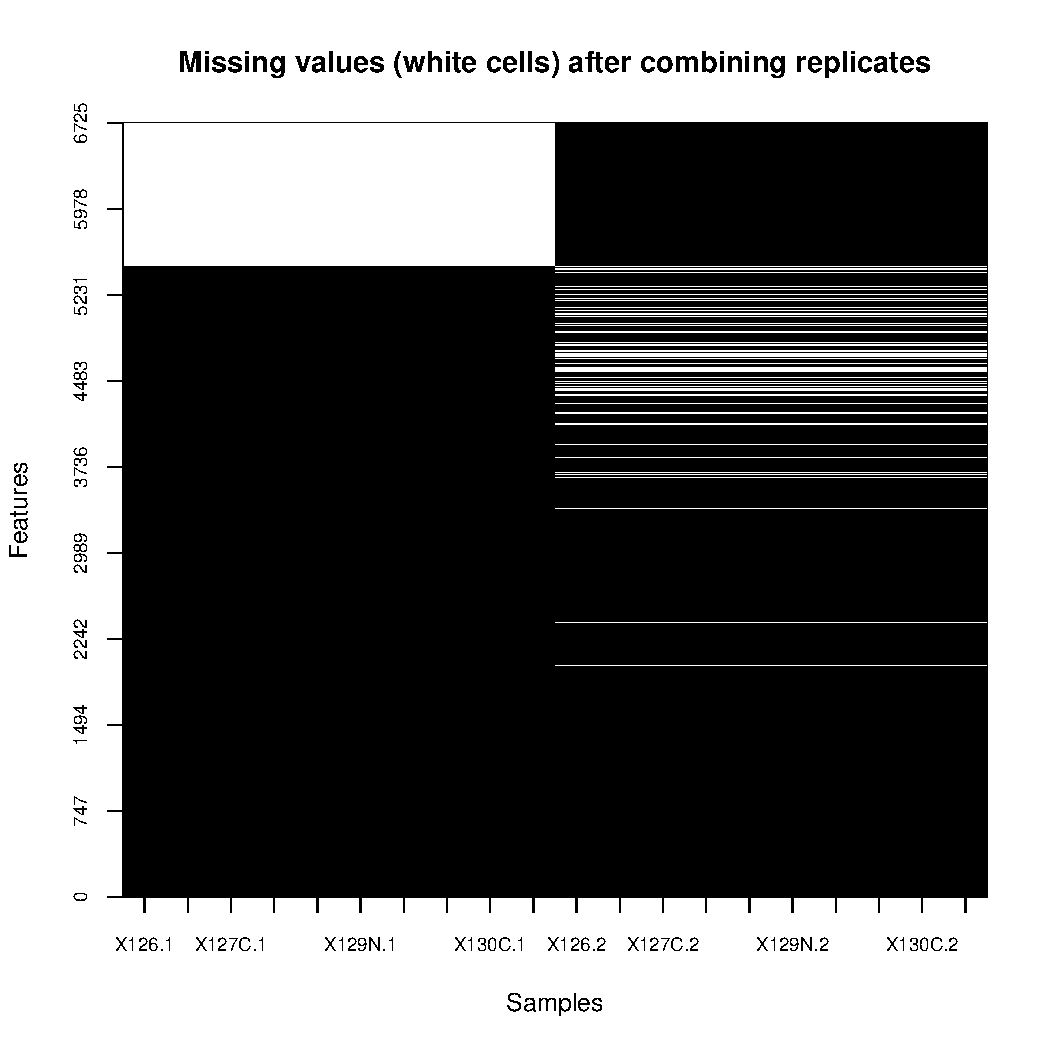
\includegraphics[width=.65\textwidth]{figure/namap-1} 

\end{knitrout}
\caption{Heatmap of missing values. Note that the features are
  re-ordered to highlight cluster of proteins with similar numbers of
  missing values.}
  \label{fig:namap}
\end{figure}

We prefer to remove proteins that were not assayed in both replicated
experiments. This is done with the \texttt{filterNA} function that
removes features (proteins) that contain more than a certain
proportion (default is 0) missing values. The \textit{Processing
  information} section summarises how combining and filtering missing
values (subsetting) changed the dimensions of the data.


\begin{knitrout}
\definecolor{shadecolor}{rgb}{0.969, 0.969, 0.969}\color{fgcolor}\begin{kframe}
\begin{alltt}
\hlstd{combined} \hlkwb{<-} \hlkwd{filterNA}\hlstd{(combined)}
\hlstd{combined}
\end{alltt}
\begin{verbatim}
## MSnSet (storageMode: lockedEnvironment)
## assayData: 5032 features, 20 samples 
##   element names: exprs 
## protocolData: none
## phenoData
##   sampleNames: X126.1 X127N.1 ... X131.2 (20 total)
##   varLabels: Replicate TMT.Reagent ... Iodixonal.Density (5 total)
##   varMetadata: labelDescription
## featureData
##   featureNames: Q9JHU4 Q9QXS1-3 ... Q9Z2R6 (5032 total)
##   fvarLabels: EntryName ProteinDescription ... ProteinCoverage2 (8
##     total)
##   fvarMetadata: labelDescription
## experimentData: use 'experimentData(object)'
## Annotation:  
## - - - Processing information - - -
## Combined [6725,20] and [6268,10] MSnSets Fri Dec  2 17:19:06 2016 
## Subset [6725,20][5032,20] Fri Dec  2 17:19:07 2016 
## Removed features with more than 0 NAs: Fri Dec  2 17:19:07 2016 
## Dropped featureData's levels Fri Dec  2 17:19:07 2016 
##  MSnbase version: 1.21.7
\end{verbatim}
\end{kframe}
\end{knitrout}

When more than 2 datasets are to be combined and too many proteins were
not consistently assayed, leading to too many proteins being filtered
out, we suggest to implement an ensemble of classifiers voting on
protein-sub-cellular niche membership over the output of several
experiments (see section \textit{Supervised machine learning} for the
description of sub-cellular assignments).

\section*{Quality Control}

Data quality is routinely examined through visualisation to verify
that sub-cellular niches have been separated along the gradient. Based
on De Duve's principle \cite{DeDuve:1981} proteins that co-localise
exhibit similar quantitation profiles across the gradient fractions
employed. One approach that has been widely used to visualise and
inspect high throughput mass spectrometry-based proteomics data is
principal components analysis (PCA). PCA is one of many dimensionality
reduction methods, that allows one to effectively summarise
multi-dimensional data in to 2 or 3 dimensions to enable
visualisation. Very generally, the original continuous
multi-dimensional data is transformed into a set of orthogonal
components ordered according to the amount of variability that they
describe. The \texttt{plot2D} and \texttt{plot3D} methods in \Biocpkg{pRoloc} allows one to
plot the principal components (PCs) of a dataset against one another,
by default the first two components are plotted on the x- and y-axis
for the \texttt{plot2D} function, and first three components are
loaded for the \texttt{plot3D} function, respectively (the
\texttt{dims} argument can be used to plot other PCs). If
distinct clusters are observed, we assume that there is organellar
separation present in the data. Although, representing the
multi-dimensional data along a limited set of PCs does not give us a
hard quantitative measure of separation, it is extremely useful
summarising complex experimental information in one figure, to get a
simplified overview of the data.

In the code chunk below we produce a 2-dimensional PCA plot of the mouse stem cell
dataset (Figure \ref{fig:pcahl}). One point on the plot represents one
protein. We can indeed see several distinct protein clusters. We
specify \texttt{fcol = NULL}, which means not to consider any feature
variable to annotate the features (proteins) with colours. We will see
later how to use this argument to annotate the PCA plot with prior information
about sub-cellular localisation.

\begin{figure}[!ht]
  \centering
\begin{knitrout}
\definecolor{shadecolor}{rgb}{0.969, 0.969, 0.969}\color{fgcolor}\begin{kframe}
\begin{alltt}
\hlkwd{library}\hlstd{(}\hlstr{"pRoloc"}\hlstd{)}
\hlkwd{plot2D}\hlstd{(hl,} \hlkwc{fcol} \hlstd{=} \hlkwa{NULL}\hlstd{,} \hlkwc{col} \hlstd{=} \hlstr{"black"}\hlstd{)}
\hlkwd{plot2D}\hlstd{(hl,} \hlkwc{method} \hlstd{=} \hlstr{"hexbin"}\hlstd{)}
\end{alltt}
\end{kframe}
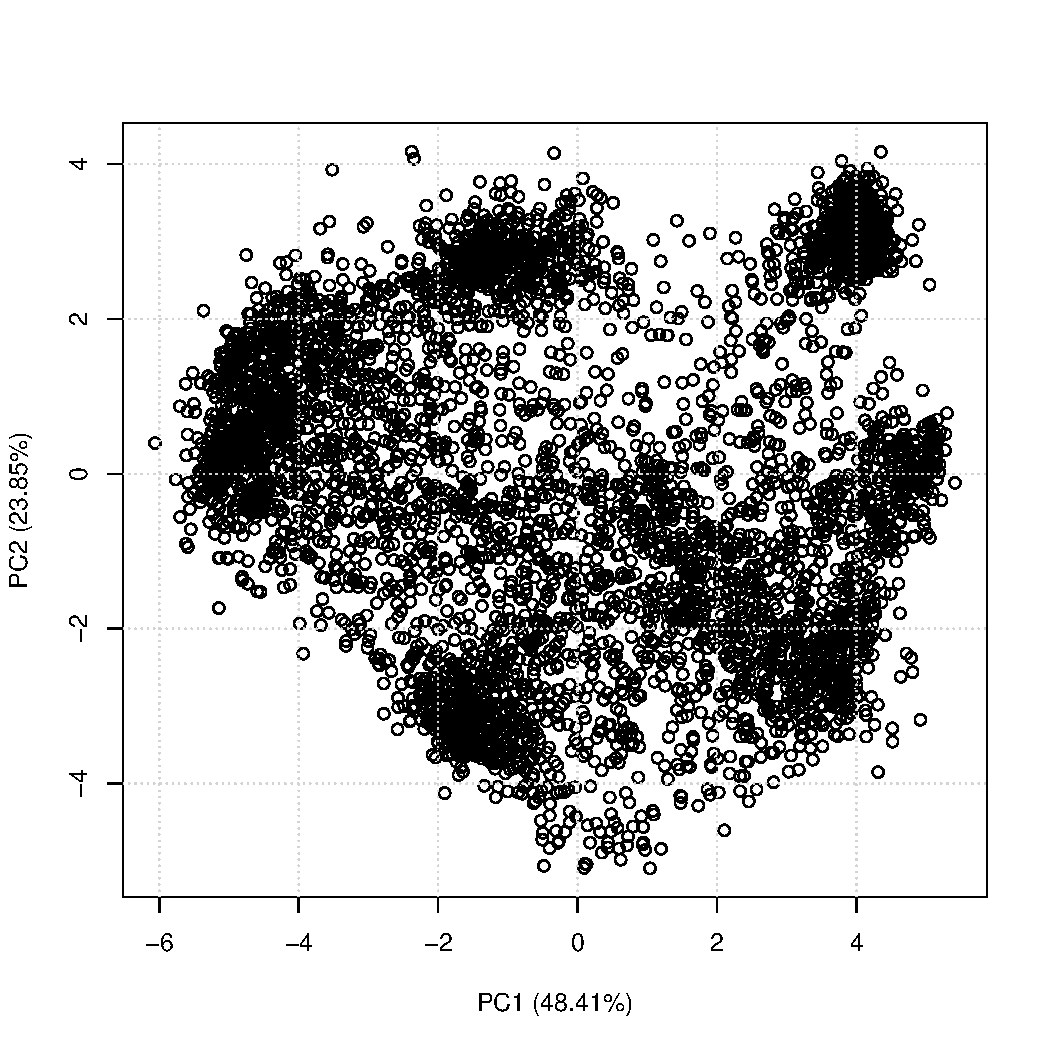
\includegraphics[width=.45\textwidth]{figure/qcplot-1} 
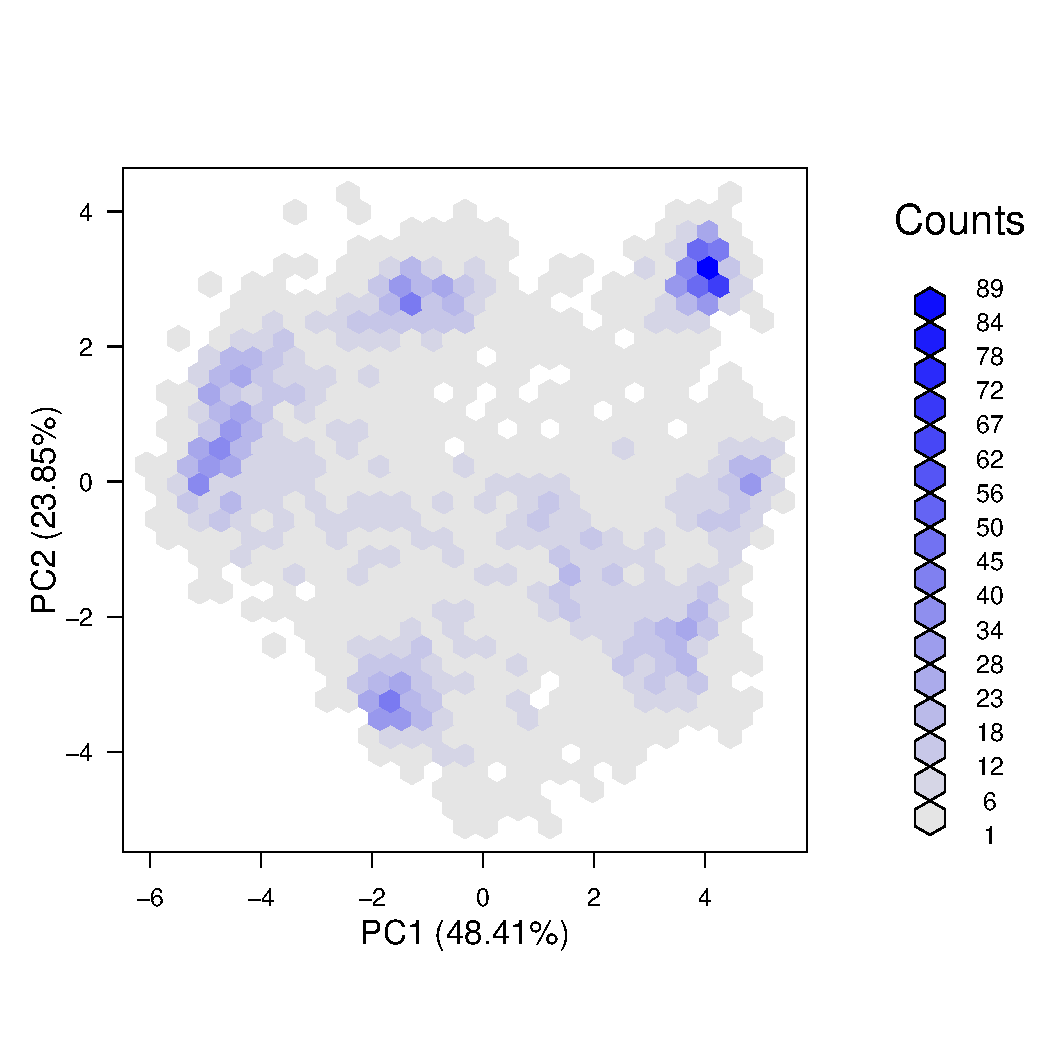
\includegraphics[width=.45\textwidth]{figure/qcplot-2} 

\end{knitrout}
\caption{PCA plot of the mouse stem cell data \texttt{hl}. Each dot
  represent a single protein, and cluster of proteins represent
  proteins residing in the same sub-cellular niche. The figure on the
  right bins proteins and represent the bins density to highlight the
  presence of protein clusters. }
  \label{fig:pcahl}
\end{figure}

In the first instance we advise one to visualise their data without
any annotation (i.e. with \texttt{fcol = NULL}), before proceeding with data
annotation. The identification of well resolved clusters in the data,
constitutes an unbiased assessment of the data structure,
demonstrating the successful separation of sub-cellular clusters.

It is also useful to visualise the relative intensities along the
gradient to identify channels displaying particularly low yield. This
can be done using the \texttt{plotDist} and \texttt{boxplot}
functions, that plot the protein profiles occupancy along the gradient
(we also display the mean channel intensities) and a \texttt{boxplot}
of the column intensities.  In the two plots displayed on figure
\ref{fig:qcbx}, we re-order the TMT channels to pair corresponding
channels in the two replicates (rather than ordering the channels by
replicate).

\begin{figure}[!ht]
  \centering
\begin{knitrout}
\definecolor{shadecolor}{rgb}{0.969, 0.969, 0.969}\color{fgcolor}\begin{kframe}
\begin{alltt}
\hlkwd{par}\hlstd{(}\hlkwc{mfrow} \hlstd{=} \hlkwd{c}\hlstd{(}\hlnum{1}\hlstd{,} \hlnum{2}\hlstd{))} \hlcom{## creates a two-panel figure}
\hlstd{o} \hlkwb{<-} \hlkwd{order}\hlstd{(hl}\hlopt{$}\hlstd{Iodixonal.Density)}
\hlkwd{plotDist}\hlstd{(hl[, o],} \hlkwc{pcol} \hlstd{=} \hlstr{"#00000010"}\hlstd{)}
\hlkwd{lines}\hlstd{(}\hlkwd{colMeans}\hlstd{(}\hlkwd{exprs}\hlstd{(hl[, o])),} \hlkwc{col} \hlstd{=} \hlstr{"red"}\hlstd{,} \hlkwc{type} \hlstd{=} \hlstr{"b"}\hlstd{)}
\hlkwd{boxplot}\hlstd{(}\hlkwd{exprs}\hlstd{(hl[, o]),} \hlkwc{las} \hlstd{=} \hlnum{2}\hlstd{)}
\end{alltt}
\end{kframe}
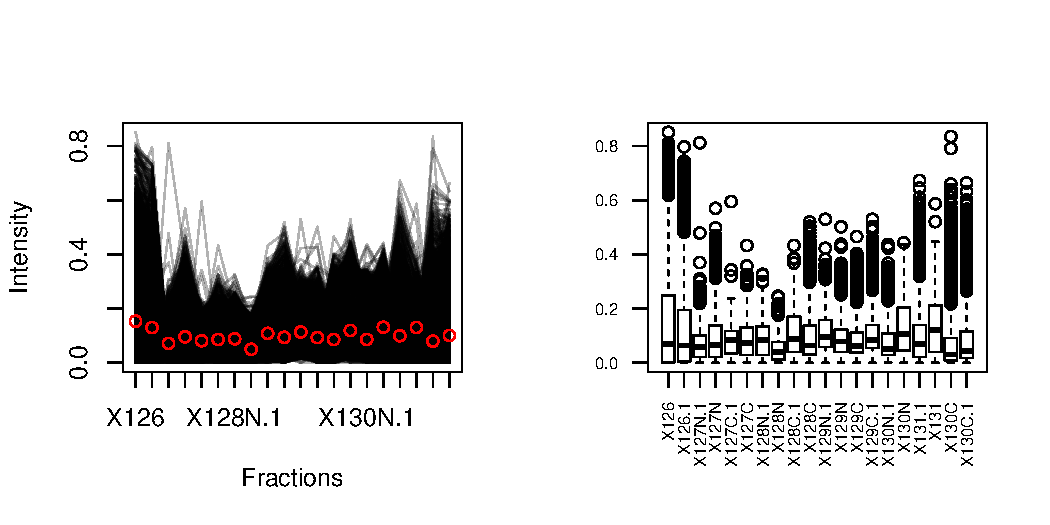
\includegraphics[width=\textwidth]{figure/qcbx-1} 

\end{knitrout}
  \caption{Protein profiles and distribution of channel intensities.}
  \label{fig:qcbx}
\end{figure}


\section*{Markers}

In the context of spatial proteomics, a marker protein is defined as a
well-known resident of a specific sub-cellular niche in a species
\textit{and} condition of interest. Applying this to machine learning
(ML), and specifically supervised learning, for the task of protein
localisation prediction, these markers constitute the labelled
training data to use as input to a classification analyses. Defining
well-known residents, and obtaining labelled training data for ML
analyses can be time consuming, but it is important to define markers
that are representative of the multivariate data space and on which a
classifier will be trained and generated. \Biocpkg{pRoloc} provides a
convenience function, \texttt{addMarkers}, to directly add markers to
an \texttt{MSnSet} object, as demonstrated in the code chunk
below. These marker sets can be accessed using the
\texttt{pRolocmarkers()} function. Marker sets are stored as a simple
named vector in R, and originate from in-house user-defined sets of
markers or from previous published studies \cite{Gatto:2014b}, which
are continuosly updated and integrated.

\begin{knitrout}
\definecolor{shadecolor}{rgb}{0.969, 0.969, 0.969}\color{fgcolor}\begin{kframe}
\begin{alltt}
\hlcom{## List available marker sets}
\hlkwd{pRolocmarkers}\hlstd{()}
\end{alltt}
\begin{verbatim}
## 7 marker lists available:
## Arabidopsis thaliana [atha]:
##  Ids: TAIR, 543 markers
## Drosophila melanogaster [dmel]:
##  Ids: Uniprot, 179 markers
## Gallus gallus [ggal]:
##  Ids: IPI, 102 markers
## Homo sapiens [hsap]:
##  Ids: Uniprot, 872 markers
## Mus musculus [mmus]:
##  Ids: Uniprot, 937 markers
## Saccharomyces cerevisiae [scer_sgd]:
##  Ids: SGD, 259 markers
## Saccharomyces cerevisiae [scer_uniprot]:
##  Ids: Uniprot Accession, 259 markers
\end{verbatim}
\end{kframe}
\end{knitrout}

These markers can then be mapped to an \texttt{MSnSet}'s
\texttt{featureNames}. The mouse dataset used here has Uniprot IDs
stored as the \texttt{featureNames} (see
\texttt{head(featureNames(hl))}) and the names of the vector of the
mouse markers stored in \Biocpkg{pRoloc} (\texttt{mmus} markers) are
also Uniprot IDs (see \texttt{head(mrk)} in the code chunk below), so
it is straightforward to match names between the markers and the
\texttt{MSnSet} instance using the \texttt{addMarkers} function. 

\begin{knitrout}
\definecolor{shadecolor}{rgb}{0.969, 0.969, 0.969}\color{fgcolor}\begin{kframe}
\begin{alltt}
\hlcom{## Use mouse markers}
\hlstd{mrk} \hlkwb{<-} \hlkwd{pRolocmarkers}\hlstd{(}\hlkwc{species} \hlstd{=} \hlstr{"mmus"}\hlstd{)}
\hlkwd{head}\hlstd{(mrk)}
\end{alltt}
\begin{verbatim}
##                 P26039                 Q6PB66                 P11276 
##   "Actin cytoskeleton"        "Mitochondrion" "Extracellular matrix" 
##                 Q6PR54                 Q05793                 P19096 
##  "Nucleus - Chromatin" "Extracellular matrix"              "Cytosol"
\end{verbatim}
\begin{alltt}
\hlcom{## Add mouse markers}
\hlstd{hl} \hlkwb{<-} \hlkwd{addMarkers}\hlstd{(hl, mrk)}
\end{alltt}


{\ttfamily\noindent\itshape\color{messagecolor}{\#\# Markers in data: 937 out of 5032}}\begin{verbatim}
## organelleMarkers
##            40S Ribosome            60S Ribosome      Actin cytoskeleton 
##                      27                      43                      13 
##                 Cytosol   Endoplasmic reticulum                Endosome 
##                      43                      95                      12 
##    Extracellular matrix         Golgi apparatus                Lysosome 
##                      10                      27                      33 
##           Mitochondrion     Nucleus - Chromatin Nucleus - Non-chromatin 
##                     383                      64                      85 
##              Peroxisome         Plasma membrane              Proteasome 
##                      17                      51                      34 
##                 unknown 
##                    4095
\end{verbatim}
\end{kframe}
\end{knitrout}

We recommend at least 13 markers per sub-cellular class (see the
\textit{Optimisation} section for details about the algorithmic
motivation of this number). Markers should be chosen to confidently
represent the distribution of genuine residents of a sub-cellular
niche. We generally recommend a conservative approach in defining
markers to avoid false assignments when assigning sub-cellular
localisation of proteins of unknown localisation. A more relaxed
definition of markers, i.e. one that broadly or over-confidently
defines markers, risks to erroneously assign proteins to a single
location, when, in reality, they reside in multiple locations
(including the assumed unique location). One can not expect to
identify exact boundaries between sub-cellular classes through marker
annotation alone; the definition of these boundaries is better handled
algorithmically, i.e. after application of the supervised learning
algorithm, using the prediction scores (as described in the
\textit{Classification} section, in particular Figure
\ref{fig:plotSVM}).

If the protein naming between the marker sets and the \texttt{MSnSet}
dataset are different e.g. the markers are labelled by Uniprot
accession numbers and the dataset entries are labelled by Uniprot
entry names, one will have to convert and match the proteins according
to the appropriate identifier. Sometimes, we find the equivalent entry
name, Uniprot ID or accession number is stored with the data, which
makes conversion between identifers relatively straightforward. If
this is not the case however, conversion can be performed using
\Biocpkg{biomaRt}, the Bioconductor
\href{http://bioconductor.org/help/workflows/annotation/Annotation_Resources/}{annotation
  resouces} or any conversion softwares available online.

\subsection*{Adding user-defined marker lists}
It is also possible for users to use their own marker list with the
\texttt{addMarkers} function. The user needs to create a named vector
of marker localisation, or a create a csv file with two columns (one
for the protein names, one for the corresponding sub-cellular marker
annotation) and pass the vector or file name respectively to the
function. As previously mentioned, the protein names of these markers
must match some (but not necessarily all) of the \texttt{MSnSet}'s
feature names. See \texttt{?addMarkers} for more details.

In general, the Gene Ontology (GO) \cite{Ashburner:2000}, and in
particular the cellular compartment (CC) namespace are a good starting
point for protein annotation and marker definition. It is important to
note however that automatic retrieval of sub-cellular localisation
information, from \Biocpkg{pRoloc} or elsewhere, is only the
beginning in defining a marker set for downstream analyses. Expert
curation is vital to check that any annotation added is in the correct
context for the biological question under investigation.


\subsection*{Visualising markers}
Having added a the mouse markers to our \texttt{fData} from the
\texttt{pRolocmarkers} we can now visualise these annotations along
the PCA plot using the \texttt{plot2D} function and then use the
\texttt{addLegend} function to map the marker classes to the
pre-defined colours. We also display the data along the first and
seventh PCs using the \texttt{dims} argument. Note that in these calls
to the \texttt{plot2D} function, we have omitted the \texttt{fcol}
argument and use of the default \texttt{"markers"} feature variable to
annotate the plot. We choose to display PCs 1 and 7 to illustrate that
while upper principal components explain much less variability in the
data (2.23\% for PC7, as opposed to 48.41\% for PC1), we see that the
mitochondrial (purple) and peroxisome (dark blue) clusters can be
differentiated, despite the apparent overlap in the visualisation of
the two first PCs (Figure \ref{fig:plotmarkers}).

\begin{figure}[!ht]
  \centering
\begin{knitrout}
\definecolor{shadecolor}{rgb}{0.969, 0.969, 0.969}\color{fgcolor}\begin{kframe}
\begin{alltt}
\hlkwd{par}\hlstd{(}\hlkwc{mfrow} \hlstd{=} \hlkwd{c}\hlstd{(}\hlnum{1}\hlstd{,} \hlnum{2}\hlstd{))}
\hlkwd{plot2D}\hlstd{(hl,} \hlkwc{main} \hlstd{=} \hlstr{"pRolocmarkers for mouse"}\hlstd{)}
\hlkwd{addLegend}\hlstd{(hl,} \hlkwc{cex} \hlstd{=} \hlnum{.6}\hlstd{)}
\hlkwd{plot2D}\hlstd{(hl,} \hlkwc{dims} \hlstd{=} \hlkwd{c}\hlstd{(}\hlnum{1}\hlstd{,} \hlnum{7}\hlstd{),} \hlkwc{main} \hlstd{=} \hlstr{"Marker resolution along PC 1 and 7"}\hlstd{)}
\end{alltt}
\end{kframe}
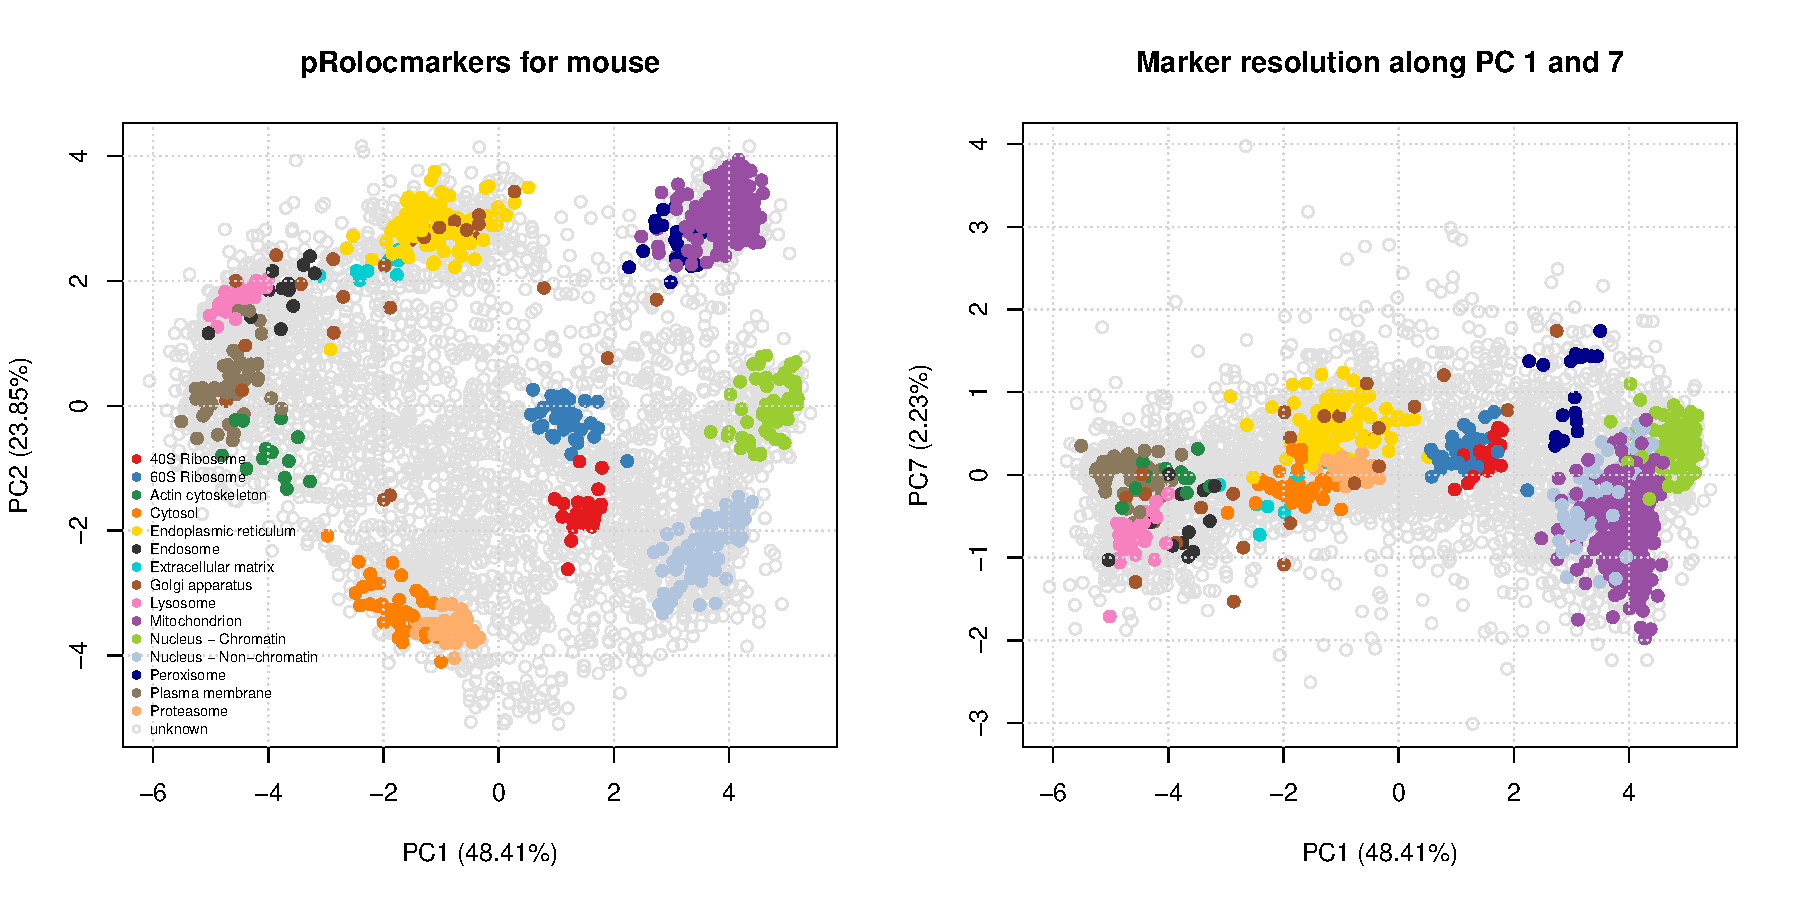
\includegraphics[width=\textwidth]{figure/plotmarkers-1} 

\end{knitrout}
\caption{Annotated PCA plots of the \texttt{hl} dataset, as produced
  with \texttt{plt2D} and \texttt{plot3D} (right).}
  \label{fig:plotmarkers}
\end{figure}


The default colours for plotting have been defined so as to enable the
differentiation of up to 30 classes. If more are provided, different
character symbols (circles, squares, ... and empty and solid symbols)
are used. The colours and the default plotting characters (solid dots
for the markers and empty circles for the features of unknown
localisation) can of course be changed, as described in the
\texttt{setStockcol} manual page.

As demonstrated in \cite{hyper} and illustrated in the PCA plot
(figure \ref{fig:plotmarkers}), the Golgi apparatus proteins (dark
brown) display a dynamic pattern, noting sets of Golgi marker proteins
that are distributed amongst other subcellular structures, an
observation supported by microscopy.  As such, we are going to reset
the annotation of Golgi markers to unknown using the
\texttt{fDataToUnknown} function. It is often used to replace empty
strings (\texttt{""}) or missing values in the markers definition to a
common definition of \textit{unknown} localisation.

\begin{knitrout}
\definecolor{shadecolor}{rgb}{0.969, 0.969, 0.969}\color{fgcolor}\begin{kframe}
\begin{alltt}
\hlstd{hl} \hlkwb{<-} \hlkwd{fDataToUnknown}\hlstd{(hl,} \hlkwc{from} \hlstd{=} \hlstr{"Golgi apparatus"}\hlstd{,} \hlkwc{to} \hlstd{=} \hlstr{"unknown"}\hlstd{)}
\hlkwd{getMarkers}\hlstd{(hl)}
\end{alltt}
\begin{verbatim}
## organelleMarkers
##            40S Ribosome            60S Ribosome      Actin cytoskeleton 
##                      27                      43                      13 
##                 Cytosol   Endoplasmic reticulum                Endosome 
##                      43                      95                      12 
##    Extracellular matrix                Lysosome           Mitochondrion 
##                      10                      33                     383 
##     Nucleus - Chromatin Nucleus - Non-chromatin              Peroxisome 
##                      64                      85                      17 
##         Plasma membrane              Proteasome                 unknown 
##                      51                      34                    4122
\end{verbatim}
\end{kframe}
\end{knitrout}


Another useful visualisation that relies on marker annotation is the
representation of the protein profiles occupancy along the gradient
using the \texttt{plotDist} function. While the PCA plot enables to
efficiently visualise the complete dataset and assess the relative
separation of different sub-cellular niches, comparing profiles of a
few marker clusters is useful to assess how exactly they differ (in
terms of peak channels, for example). On figure \ref{fig:plotDist2},
we plot the profile of the mitochondrial and peroxisome markers to
highlight the differences in profiles between these two sets of
markers in the channels labelled with tag 129C, as represented above
along the 7th PC on the PCA plot on figure \ref{fig:plotmarkers}.

\begin{figure}[!ht]
  \centering
\begin{knitrout}
\definecolor{shadecolor}{rgb}{0.969, 0.969, 0.969}\color{fgcolor}\begin{kframe}
\begin{alltt}
\hlstd{hlo} \hlkwb{<-} \hlstd{hl[,} \hlkwd{order}\hlstd{(hl}\hlopt{$}\hlstd{Iodixonal.Density)]}
\hlkwd{plotDist}\hlstd{(hlo[}\hlkwd{fData}\hlstd{(hlo)}\hlopt{$}\hlstd{markers} \hlopt{==} \hlstr{"Mitochondrion"}\hlstd{, ],}
         \hlkwc{pcol} \hlstd{=} \hlstr{"purple"}\hlstd{,} \hlkwc{fractions} \hlstd{=} \hlstr{"Tag"}\hlstd{)}
\hlkwd{title}\hlstd{(}\hlkwc{main} \hlstd{=} \hlstr{"Marker occupancy profiles along the gradient"}\hlstd{)}
\hlkwd{matlines}\hlstd{(}\hlkwd{t}\hlstd{(}\hlkwd{exprs}\hlstd{(hlo[}\hlkwd{fData}\hlstd{(hlo)}\hlopt{$}\hlstd{markers} \hlopt{==} \hlstr{"Peroxisome"}\hlstd{, ])),}
         \hlkwc{lty} \hlstd{=} \hlnum{1}\hlstd{,} \hlkwc{col} \hlstd{=} \hlstr{"darkblue"}\hlstd{,} \hlkwc{type} \hlstd{=} \hlstr{"l"}\hlstd{)}
\hlkwd{legend}\hlstd{(}\hlstr{"topleft"}\hlstd{,} \hlkwd{c}\hlstd{(}\hlstr{"Mitochondrion"}\hlstd{,} \hlstr{"Peroxisome"}\hlstd{),}
       \hlkwc{lty} \hlstd{=} \hlnum{1}\hlstd{,} \hlkwc{col} \hlstd{=} \hlkwd{c}\hlstd{(}\hlstr{"purple"}\hlstd{,} \hlstr{"blue"}\hlstd{),} \hlkwc{bty} \hlstd{=} \hlstr{"n"}\hlstd{)}
\end{alltt}
\end{kframe}
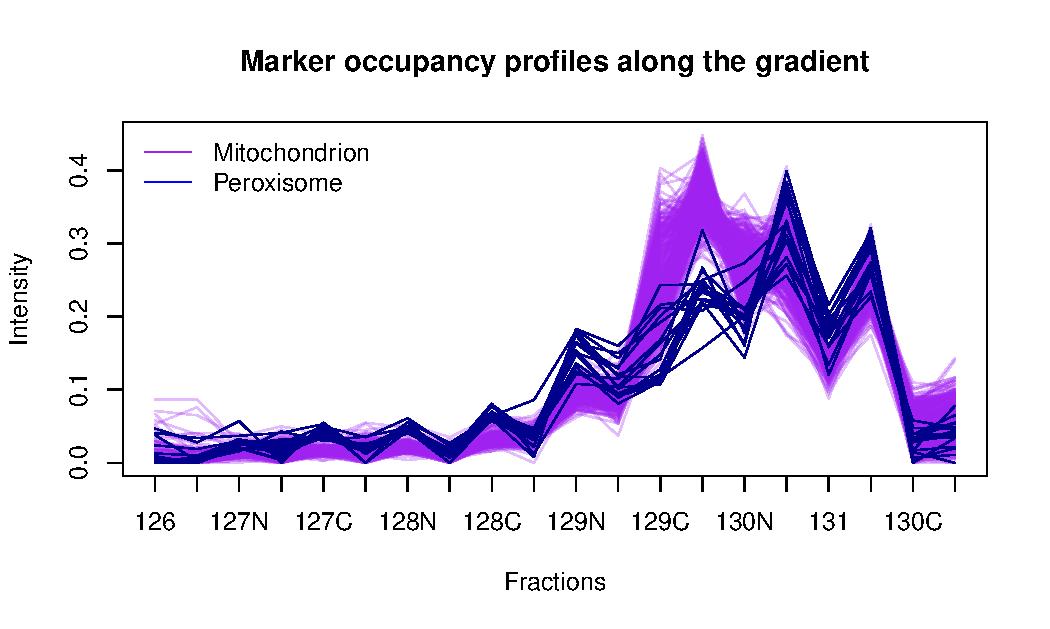
\includegraphics[width=.6\textwidth]{figure/plotDist-1} 

\end{knitrout}
  \caption{Mitochondrion and peroxisome protein profiles.}
  \label{fig:plotDist2}
\end{figure}

Finally, in addition to \texttt{plot2D}, the \texttt{plot3D} function
allows to interactively explore a 3-dimensional plot of the data.

\subsection*{Features of interest}
In addition to adding annotation using the \texttt{addMarkers}
function, one can store specific sets of proteins by using the
\textit{Features of interest} infrastructure from the
\Biocpkg{MSnbase} package. If users have specific subsets of proteins
they wish to highlight in their data (possibly across multiple
experiments) they would first create a \texttt{FeaturesOfInterest}
object. For example, if we wanted to highlight a proteins with the
accession numbers Q8CG48, Q8CG47, Q8K2Z4, and Q8C156, which are some
of the proteins known to form part of the 13S condensin complex, we
would create a first create a \texttt{FeaturesOfInterest} object, and
subsequently highlight their location on a PCA plot with the
\texttt{highlightOnPlot} function.

\begin{figure}[!ht]
  \centering
\begin{knitrout}
\definecolor{shadecolor}{rgb}{0.969, 0.969, 0.969}\color{fgcolor}\begin{kframe}
\begin{alltt}
\hlstd{prots} \hlkwb{<-} \hlkwd{c}\hlstd{(}\hlstr{"Q8CG48"}\hlstd{,} \hlstr{"Q8CG47"}\hlstd{,} \hlstr{"Q8K2Z4"}\hlstd{,} \hlstr{"Q8C156"}\hlstd{)}
\hlstd{foi13s} \hlkwb{<-} \hlkwd{FeaturesOfInterest}\hlstd{(}\hlkwc{description} \hlstd{=} \hlstr{"13S consensin proteins"}\hlstd{,}
                             \hlkwc{fnames} \hlstd{= prots,}
                             \hlkwc{object} \hlstd{= hl)}
\hlstd{foi13s}
\end{alltt}
\begin{verbatim}
## Traceable object of class "FeaturesOfInterest"
##  Created on Fri Dec  2 17:19:09 2016 
##  Description:
##   13S consensin proteins
##  4 features of interest:
##    Q8CG48, Q8CG47, Q8K2Z4, Q8C156
\end{verbatim}
\begin{alltt}
\hlkwd{plot2D}\hlstd{(hl)}
\hlkwd{addLegend}\hlstd{(hl,} \hlkwc{cex} \hlstd{=} \hlnum{.6}\hlstd{)}
\hlkwd{highlightOnPlot}\hlstd{(hl, foi13s)}
\end{alltt}
\end{kframe}
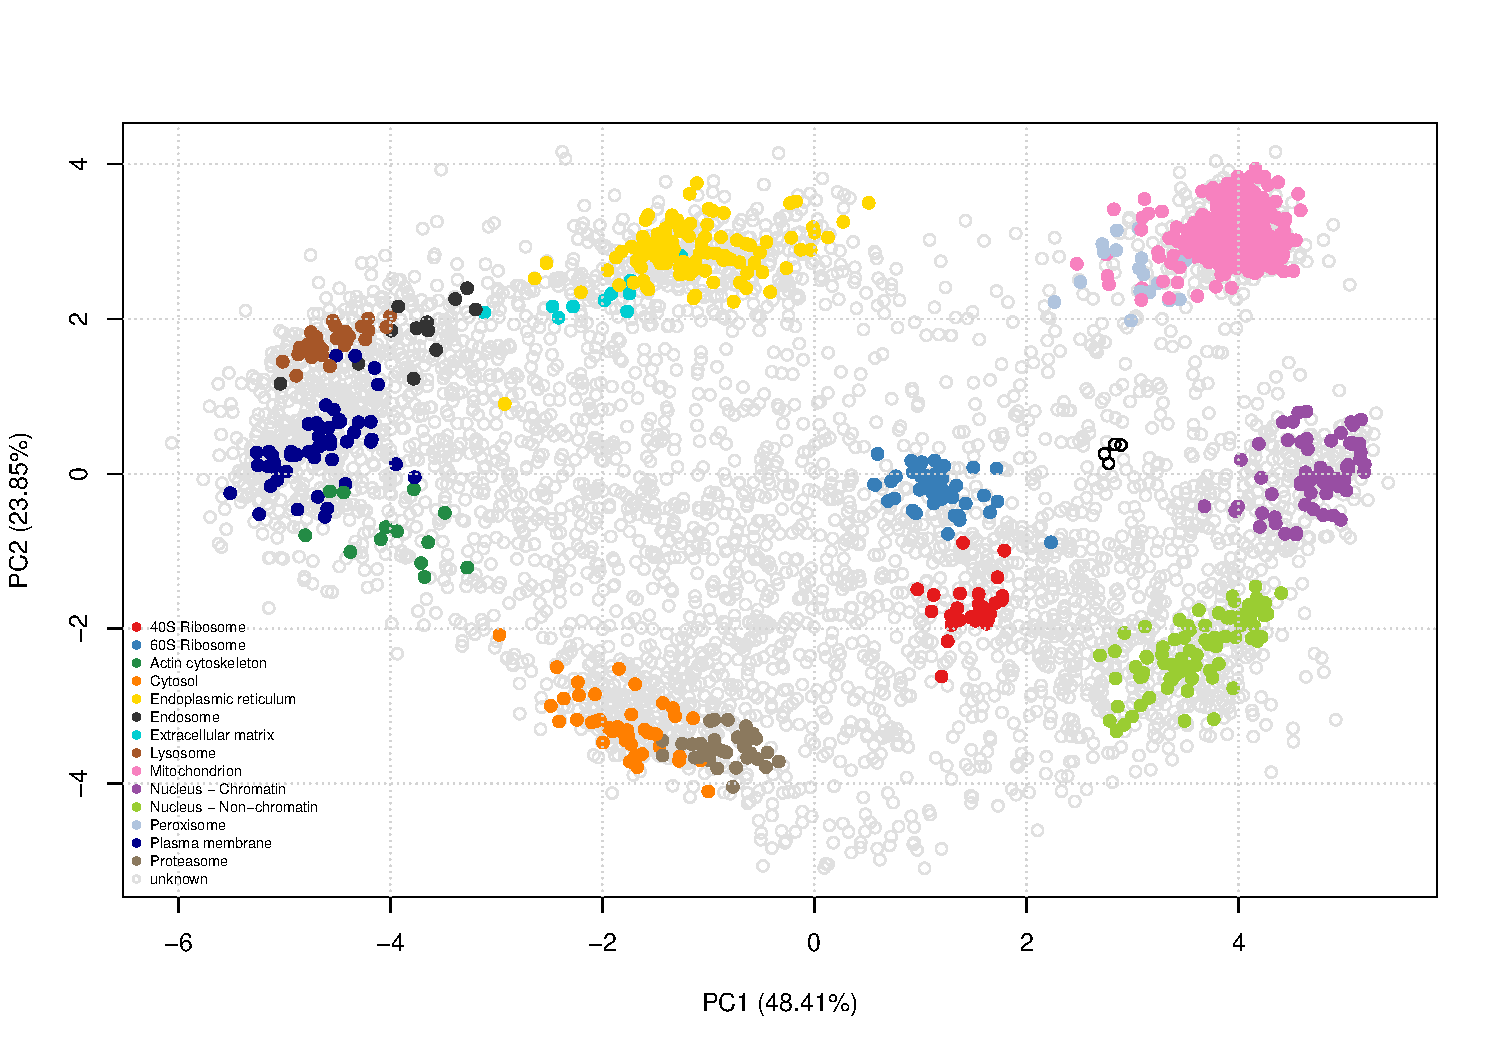
\includegraphics[width=.8\textwidth]{figure/foi-1} 

\end{knitrout}
  \caption{Highlighting protein features of interest.}
  \label{fig:foi}
\end{figure}

Users can also create several sets of \texttt{FeaturesOfInterest}
object and store them in a \texttt{FoICollection}.

It is also worthy of note that it is possible to search for a
specific protein of interest by \texttt{featureNames} or using any
identifying information found in the \texttt{fData} columns by using
the search box on the \texttt{pRolocVis} application part of the
\Biocpkg{pRolocGUI} package (see section on interactive
visualisation). This can be handy for quickly searching and
highlighting proteins on the fly, the disavanatge here is that
proteins can only be searched for a one-by-one basis.

\section*{Replication}

With the aim of maximising the sub-cellular resolution and,
consequently, the reliability in protein sub-cellular assignments, we
follow the advice in \cite{Trotter:2010} and combine replicated spatial
proteomics experiments as described above. Indeed, Trotter et
al. have shown a significant improvement in protein–organelle
association upon direct combination of single experiments, in
particular when these resolve different subcellular niches.

Direct comparisons of individual channels in replicated experiments
does not provide an adequate, goal-driven assessment of different
experiments. Indeed, due to the nature of the experiment and gradient
fraction collection, the quantitative channels do not correspond to
identical selected fractions along the gradient. For example, in the
table below (taken from \texttt{hl}'s \texttt{pData}) TMT channels
127C (among others) in both replicates originate from different sets
of gradient fractions (gradient fractions 7 - 9 and 8 - 9 for each
replicate, respectively). Different sets of gradient fractions are
often pooled to obtain enough material and optimise acurate
quantitation.

% latex table generated in R 3.3.2 by xtable 1.8-2 package
% Fri Dec  2 17:19:09 2016
\begin{table}[ht]
\centering
\begin{tabular}{rrllr}
  \hline
 & Replicate & Tag & Gradient.Fraction & Iodixonal.Density \\ 
  \hline
X127C &   1 & 127C & 8 to 9 (pooled) & 11.00 \\ 
  X127C.1 &   2 & 127C & 7 to 9 (pooled) & 10.00 \\ 
   \hline
\end{tabular}
\caption{Differences in gradient fraction pooling.} 
\label{tab:pdtab}
\end{table}


The more relevant comparison unit is not a single channel, but rather
the complete protein occupancy profiles, which are best visualised 
experiment-wide on a PCA plot. As such, we prefer to focus on the
direct, qualitative comparison of individual replicate PCA plots,
assuring that each displays acceptable sub-cellular resolution. Note
that in the code chunk below, we mirror the x-axis to represent the
two figures with the same orientation. The interactive "compare"
application part of the \Biocpkg{pRolocGUI} package is also useful for
examining replicate experiments (see the next section interactive
visualisation for details).

\begin{figure}[!ht]
  \centering
\begin{knitrout}
\definecolor{shadecolor}{rgb}{0.969, 0.969, 0.969}\color{fgcolor}\begin{kframe}
\begin{alltt}
\hlkwd{par}\hlstd{(}\hlkwc{mfrow} \hlstd{=} \hlkwd{c}\hlstd{(}\hlnum{1}\hlstd{,} \hlnum{2}\hlstd{))}
\hlkwd{plot2D}\hlstd{(hl[, hl}\hlopt{$}\hlstd{Replicate} \hlopt{==} \hlnum{1}\hlstd{],} \hlkwc{main} \hlstd{=} \hlstr{"Replicate 1"}\hlstd{)}
\hlkwd{plot2D}\hlstd{(hl[, hl}\hlopt{$}\hlstd{Replicate} \hlopt{==} \hlnum{2}\hlstd{],} \hlkwc{main} \hlstd{=} \hlstr{"Replicate 2"}\hlstd{,} \hlkwc{mirrorX} \hlstd{=} \hlnum{TRUE}\hlstd{)}
\end{alltt}
\end{kframe}
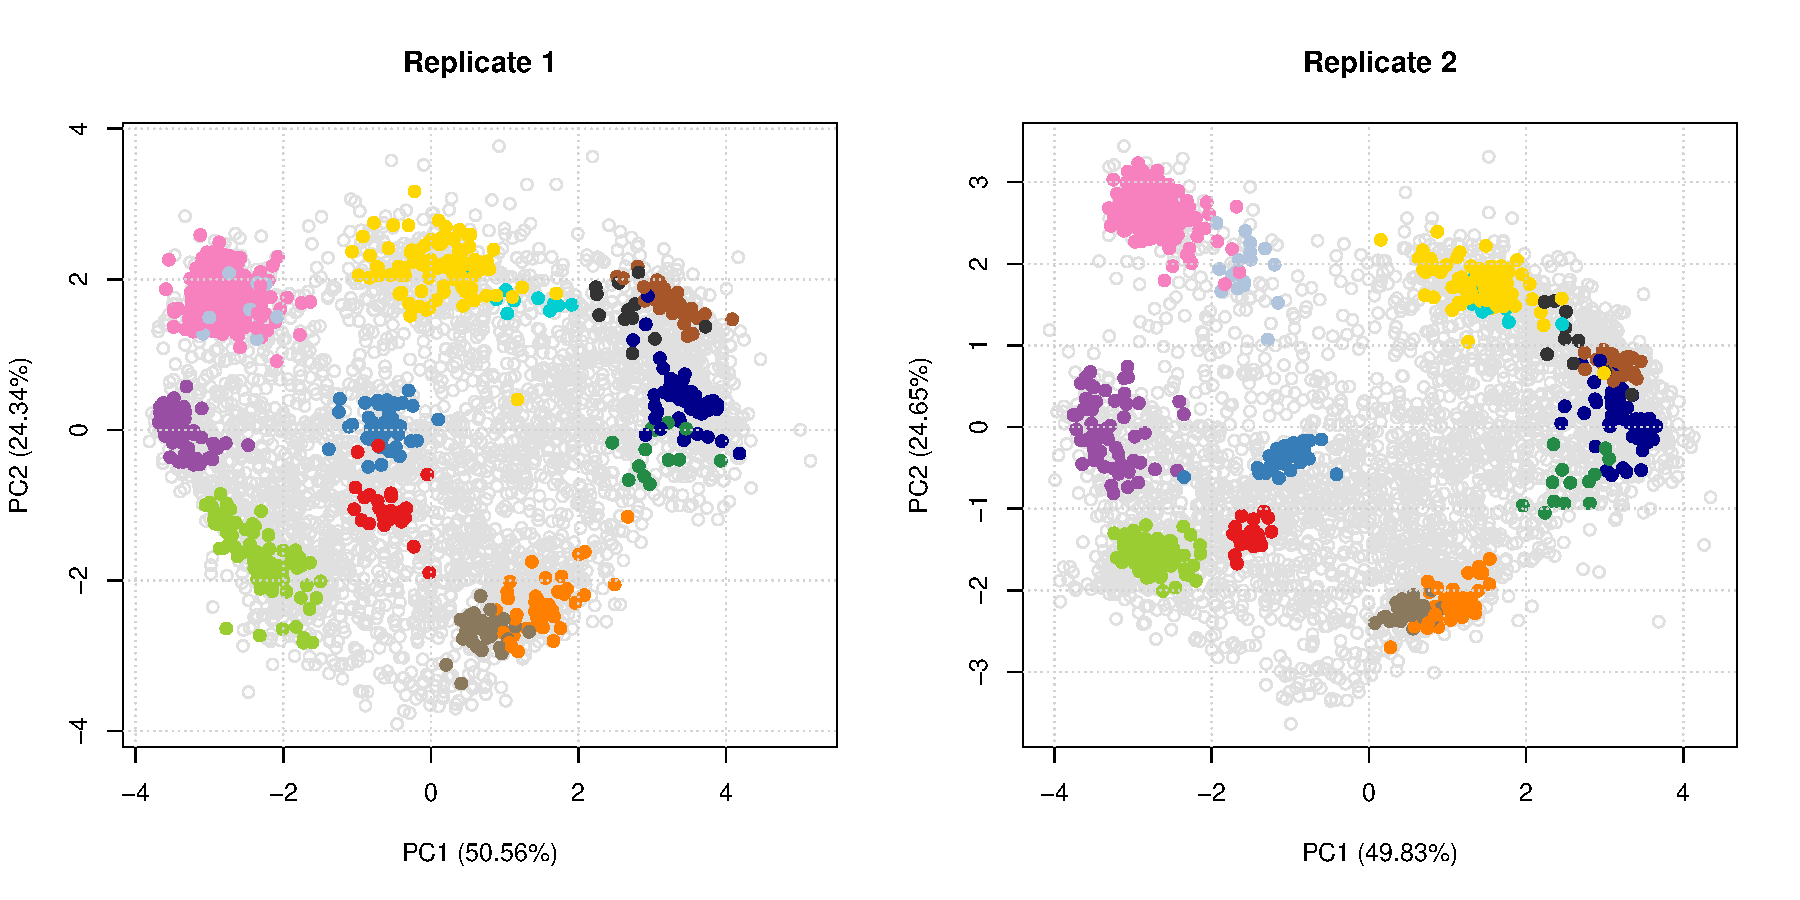
\includegraphics[width=\textwidth]{figure/plot2Drep-1} 

\end{knitrout}
  \caption{PCA plots of replicates 1 and 2}
  \label{fig:plot2Drep}
\end{figure}


\clearpage

\section*{Interactive visualisation}

Visualisation and data exploration is an important aspect of data
analyses allowing one to shed light on data structure and patterns of
interest. Using the \Biocpkg{pRolocGUI} package we can interactively
visualise, explore and interrogate quantitative spatial proteomics
data. The \Biocpkg{pRolocGUI} package is currently under active
development and it relies on the \texttt{shiny} framework for
reactivity and interactivity. The package currently distributes 3
different GUI's (\textit{main} (default), \textit{compare} or
\textit{compare}) which are wrapped and launched by the
\texttt{pRolocVis} function. 

\subsubsection*{The main application}
In the below code chunk we lauch the main
app (note, we do not need to specify the argument, \texttt{app =
  "main"} as it is the default).

\begin{knitrout}
\definecolor{shadecolor}{rgb}{0.969, 0.969, 0.969}\color{fgcolor}\begin{kframe}
\begin{alltt}
\hlkwd{library}\hlstd{(}\hlstr{"pRolocGUI"}\hlstd{)}
\hlkwd{pRolocVis}\hlstd{(hl)}
\end{alltt}
\end{kframe}
\end{knitrout}

\begin{figure}[!ht]
  \centering
  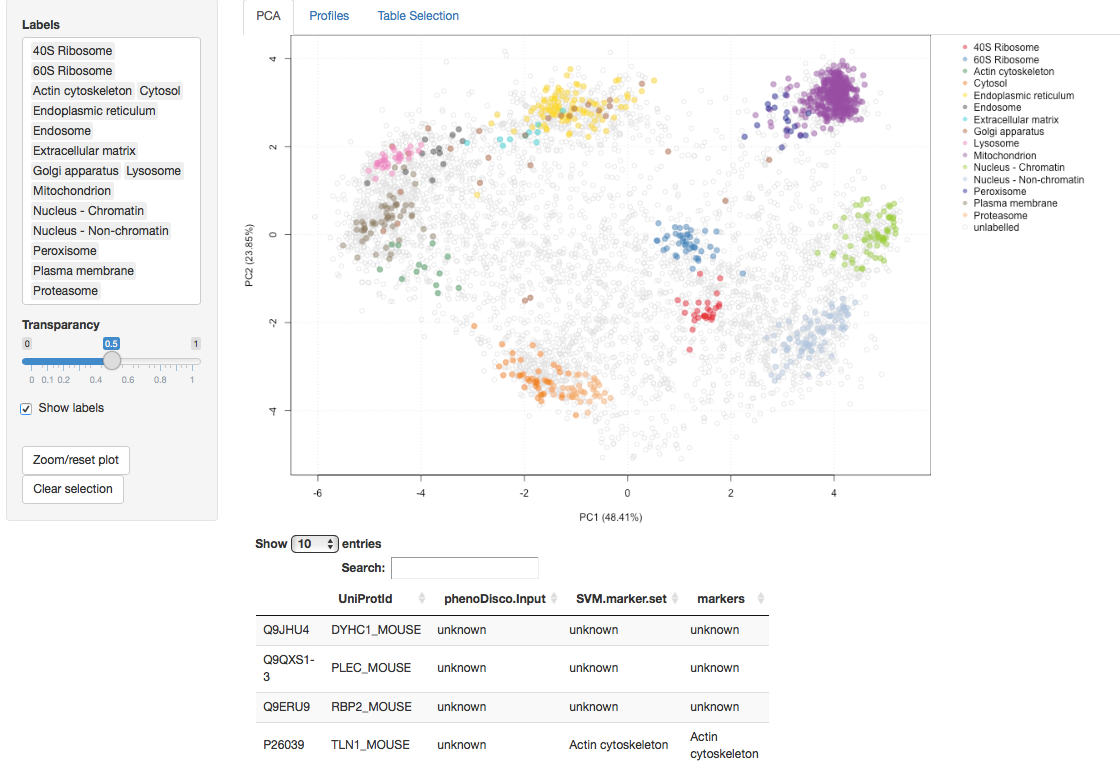
\includegraphics[width=\textwidth]{./Figures/mainapp.png}
  \caption{A screen shot of clickable interface and zoomable PCA plot
    of the main app in the \Biocpkg{pRolocGUI} package. }
  \label{fig:app}
\end{figure}

As diplayed in the screenshot in figure \ref{fig:app}, the
\textit{main} application is designed for exploratory data analysis
and is divied into 3 tabs: (1) PCA, (2) Profiles and (3) Table
selection. The default view upon loading is the PCA tab, which
features a clickable interface and zoomable PCA plot with an
interactive data table for displaying the quantitation information.
Particular proteins of interest can be highlighted using the text
search box. There is also an alternate profiles tab for visualisation
of the protein profiles, which can be used to examine the patterns of
proteins of interest. The Table selection tab provides an interface to
control data table column selection. A short
animation\footnote{\url{https://github.com/lmsimp/bioc-pRoloc-hyperLOPIT-workflow/blob/master/Figures/pRolocVis\_pca.gif}}
illustrating the interface is available in the manuscript repository~\cite{ghrepo}.

\subsubsection*{The compare application}
The \textit{compare} application is useful for examining two replicate
experiments, or two experiments from different conditions, treatments
etc. The compare application is called by default if the input object
to \texttt{pRolocVis} is an \texttt{MSnSetList} of 2 \texttt{MSnSets},
but it can also be specified by calling the argument \texttt{app =
  "compare"}. For example, in the code chunk below we first create an
\texttt{MSnSetList} of replicates 1 and 2 of the hyperLOPIT data, this
is then passed to \texttt{pRolocVis}.

\begin{knitrout}
\definecolor{shadecolor}{rgb}{0.969, 0.969, 0.969}\color{fgcolor}\begin{kframe}
\begin{alltt}
\hlkwd{data}\hlstd{(hyperLOPIT2015ms3r1)}
\hlkwd{data}\hlstd{(hyperLOPIT2015ms3r2)}
\hlstd{hllst} \hlkwb{<-} \hlkwd{MSnSetList}\hlstd{(}\hlkwd{list}\hlstd{(hyperLOPIT2015ms3r1, hyperLOPIT2015ms3r2))}
\hlkwd{pRolocVis}\hlstd{(hllst,} \hlkwc{app} \hlstd{=} \hlstr{"compare"}\hlstd{)}
\end{alltt}
\end{kframe}
\end{knitrout}

\begin{figure}[!ht]
  \centering
  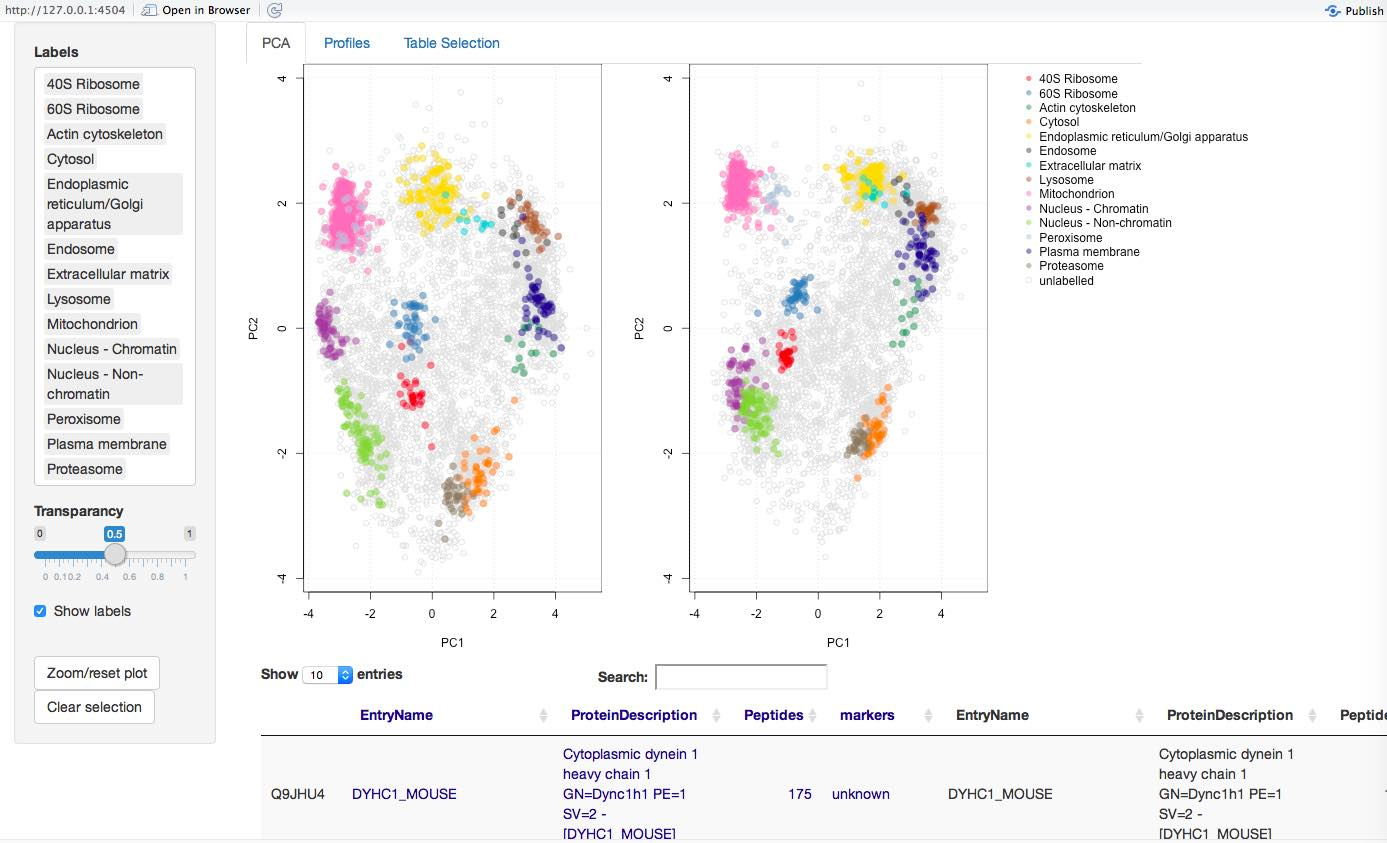
\includegraphics[width=\textwidth]{./Figures/SS_Compare1.jpg}
  \caption{The compare application, main panel}
  \label{fig:compare}
\end{figure}

The comparison app loads the two PCA plots side-by-side. Only common
proteins between the two data sets are displayed. As per the main
application, proteins can be searched, identified and highlighted on
both PCA plots and in the dedicated profiles tab. One key feature of
the compare application is the ability to re-map the second dataset
onto the PCA data space of the first (reference) data set (see
\texttt{?pRolocVis} and the argument \texttt{remap = TRUE}). Using the first dataset
as the reference set, PCA is carried out on the first dataset and the
standard deviations of the principal components (i.e. the square roots
of the eigenvalues of the covariance/correlation matrix) and the
matrix of variable loadings (i.e. a matrix whose columns contain the
eigenvectors) are stored and then used to calculate the principal
components of the second dataset. Both datasets are scaled and
centered in the usual way. The first dataset appears on the left, and
the second re-mapped data appears on the right. The order of the first
(the reference data for remapping) and second dataset can be changed
through regeneration/re-ordering of the \texttt{MSnSetList} object.

\subsubsection*{The classify application}
The final application \textit{classify}, has been designed to view
machine learning classification results according to user-specified
thresholds for the assignment of proteins to its sub-cellular
location, as discussed later in the subsection \textit{thresholding}
in the \textit{supervised machine learning section}.


\section*{Novelty Detection}

The extraction of sub-cellular protein clusters can be difficult owing
to the limited number of marker proteins that exist in databases and
elsewhere. Furthermore, given the vast complexity of the cell,
automatic annotation retrieval does not always give a full
representation of the true sub-cellular diversity in the data. For
downstream analyses, such as supervised machine learning, it is
desirable to obtain reliable markers that cover as many sub-cellular
niches as possible, as these markers are directly used in the training
phase of the ML classification. We find that a lack of sub-cellular
diversity in the labelled training data leads to prediction errors, as
unlabelled instances can only be assigned to a class that exists in
the training data \cite{Breckels:2013}. In such scenarios, novelty
detection can be useful to identify data-specific sub-cellular
groupings such as organelles and protein complexes. The phenotype
discovery (phenoDisco) algorithm \cite{Breckels:2013} is one such method
and is available in \Biocpkg{pRoloc}. It is an iterative
semi-supervised learning method that combines the classification of
proteins on existing labelled data with the detection of new clusters.

In addition to extracting new phenotypes, novelty detection methods
are also useful for confirming the presence of known or postulated
clusters in an unbiased fashion. For example, in \cite{hyper} the
\texttt{phenoDisco} algorithm was used to confirm the data-specific presence
of the nucleus and nucleus sub-compartments. In the code chunk below,
we demonstrate how to do this analysis, highlighting some of the
optional arguments and parameters available for phenotype extraction
and give some advice on how to interpret the output.

As the \texttt{phenoDisco} algorithm is semi-supervised it uses both labelled
(markers) and unlabelled data to explore the data structure and find
new sub-cellular data clusters. Thus the first step is to define some
input labelled data i.e. markers, that the algorithm will use as input
for the supervised learning aspect of the algorithm. As described in
\cite{hyper} we define a set of markers to use as input for the analyses
that cover well-known residents from three distinct organelle
structures; the mitochondria, plasma membrane and ER, and from three
well-known and abundant protein complexes; the proteasome and two
ribosomal subunits, 40S and 60S.  These input markers are stored in
the \texttt{featureData} column of \texttt{hl} where \texttt{fcol = "phenoDisco.Input"}. We
can use the convenience accessor function \texttt{getMarkers} to print out a
table of the markers contained in this marker set. These initial
markers were manually curated using information from the UniProt
database, the Gene Ontology and the literature. 

\begin{knitrout}
\definecolor{shadecolor}{rgb}{0.969, 0.969, 0.969}\color{fgcolor}\begin{kframe}
\begin{alltt}
\hlkwd{getMarkers}\hlstd{(hl,} \hlkwc{fcol} \hlstd{=} \hlstr{"phenoDisco.Input"}\hlstd{)}
\end{alltt}
\begin{verbatim}
## organelleMarkers
##                          40S Ribosome 
##                                    26 
##                          60S Ribosome 
##                                    43 
## Endoplasmic reticulum/Golgi apparatus 
##                                    76 
##                         Mitochondrion 
##                                   261 
##                       Plasma membrane 
##                                    50 
##                            Proteasome 
##                                    34 
##                               unknown 
##                                  4542
\end{verbatim}
\end{kframe}
\end{knitrout}

In the code chunk below we show how to run the \texttt{phenoDisco}
function and return a novelty detection result, according to the
specified parameters. The algorithm parameters \texttt{times}, \texttt{GS} and \texttt{p}
are passed to the function, along with the \texttt{fcol} to tell the
algorithm where the input training data is contained. 

\begin{knitrout}
\definecolor{shadecolor}{rgb}{0.969, 0.969, 0.969}\color{fgcolor}\begin{kframe}
\begin{alltt}
\hlcom{## As per Christoforou et al (2016), }
\hlstd{hl} \hlkwb{<-} \hlkwd{phenoDisco}\hlstd{(hl,} \hlkwc{fcol} \hlstd{=} \hlstr{"phenoDisco.Input"}\hlstd{,} \hlkwc{times} \hlstd{=} \hlnum{200}\hlstd{,} \hlkwc{GS} \hlstd{=} \hlnum{60}\hlstd{)}
\end{alltt}
\end{kframe}
\end{knitrout}

Note: We do not evaluate this code chunk in this document as the
algorithm is computationally intensive and best parallelised over
multiple workers. This phenoDisco analysis took ~24 hours to complete
when parallelised over 40 workers.

The argument \texttt{times} indicates the number of times we run
unsupervied Gaussian Mixture Modelling before defining a new phenotype
cluster.  The recommended minimum and default value is 100. In the
above code chunk we increase the value to \texttt{times = 200} as we
have found for larger datasets (e.g. 5000+ proteins) a higher
\texttt{times} is requried for convergence. \texttt{GS} defines the
minimum number of proteins allowed per new data cluster and thus
heavily influences what type of new clusters are extracted. For
example, if a user is interesed in the detection of small complexes
they may wish to use a small \texttt{GS = 10}, or \texttt{= 20} etc.
If they wish to detect larger, more abundant sub-cellular niches a
much higher \texttt{GS} would be preferable. Specifying a small
\texttt{GS} can be more time consuming than using a larger
\texttt{GS}, and there is a trade off between finding interesting
small complexes and those that may not be of interest as we find there
is a tendancy to find more noise when using a small \texttt{GS}
compared to using a higher one.

One may also consider increasing the search space for new data
clusters by increasing the value of the parameter \texttt{G}. This
defines the number of GMM components to test and fit; the default is
\texttt{G = 1:9} (the default value in the
\href{https://cran.r-project.org/web/packages/mclust/index.html}{\textit{mclust}}
package \cite{mclust}). One should note that the decreasing the
\texttt{GS}, and increasing the values of the arguments
\texttt{times}, \texttt{G} (among other function arguments, see
\texttt{?phenoDisco}) will heavily influence (increase) the total time
taken to run the algorithm.  \texttt{phenoDisco} supports
parallelisation and we strongly suggest you make use of a parallel
processing to run these analyses.



The ouput of running the \texttt{phenoDisco} algorithm is an
\texttt{MSnSet} containing the new data clusters, appended to the
\texttt{featureData} under the name \texttt{pd}. The results can be
displayed by using the \texttt{getMarkers} function. We see that 5 new
phenotype data clusters were found.

\begin{knitrout}
\definecolor{shadecolor}{rgb}{0.969, 0.969, 0.969}\color{fgcolor}\begin{kframe}
\begin{alltt}
\hlstd{hl}
\end{alltt}
\begin{verbatim}
## MSnSet (storageMode: lockedEnvironment)
## assayData: 5032 features, 20 samples 
##   element names: exprs 
## protocolData: none
## phenoData
##   sampleNames: X126 X127N ... X131.1 (20 total)
##   varLabels: Replicate Tag Gradient.Fraction Iodixonal.Density
##   varMetadata: labelDescription
## featureData
##   featureNames: Q9JHU4 Q9QXS1-3 ... Q9Z2R6 (5032 total)
##   fvarLabels: uniprot.accession uniprot.id ... pd (27 total)
##   fvarMetadata: labelDescription
## experimentData: use 'experimentData(object)'
## Annotation:  
## - - - Processing information - - -
## Added markers from  'mrk' marker vector. Fri Dec  2 17:19:08 2016 
## Added markers from  'pdres' marker vector. Fri Dec  2 17:19:09 2016 
##  MSnbase version: 2.1.4
\end{verbatim}
\begin{alltt}
\hlkwd{getMarkers}\hlstd{(hl,} \hlkwc{fcol} \hlstd{=} \hlstr{"pd"}\hlstd{)}
\end{alltt}
\begin{verbatim}
## organelleMarkers
##                          40S Ribosome 
##                                   106 
##                          60S Ribosome 
##                                    95 
## Endoplasmic reticulum/Golgi apparatus 
##                                   393 
##                         Mitochondrion 
##                                   525 
##                           Phenotype 1 
##                                   300 
##                           Phenotype 2 
##                                   253 
##                           Phenotype 3 
##                                   203 
##                           Phenotype 4 
##                                    74 
##                           Phenotype 5 
##                                    91 
##                       Plasma membrane 
##                                   421 
##                            Proteasome 
##                                    92 
##                               unknown 
##                                  2479
\end{verbatim}
\end{kframe}
\end{knitrout}


\begin{figure}[!ht]
  \centering
\begin{knitrout}
\definecolor{shadecolor}{rgb}{0.969, 0.969, 0.969}\color{fgcolor}\begin{kframe}
\begin{alltt}
\hlcom{## Re-order the colours for the phenoDisco output}
\hlstd{cl} \hlkwb{<-} \hlkwd{getMarkerClasses}\hlstd{(hl,} \hlstr{"pd"}\hlstd{)}
\hlstd{cols} \hlkwb{<-} \hlkwd{getStockcol}\hlstd{()[}\hlkwd{seq}\hlstd{(cl)]}
\hlstd{ind} \hlkwb{<-} \hlkwd{grep}\hlstd{(}\hlstr{"Pheno"}\hlstd{, cl,} \hlkwc{invert} \hlstd{=} \hlnum{TRUE}\hlstd{)}
\hlstd{cols[ind]} \hlkwb{<-} \hlkwd{getStockcol}\hlstd{()[}\hlkwd{seq}\hlstd{(cl)][}\hlnum{1}\hlopt{:}\hlkwd{length}\hlstd{(ind)]}
\hlstd{cols[}\hlopt{-}\hlstd{ind]} \hlkwb{<-} \hlkwd{getStockcol}\hlstd{()[}\hlkwd{seq}\hlstd{(cl)][(}\hlkwd{length}\hlstd{(ind)} \hlopt{+} \hlnum{1}\hlstd{)}\hlopt{:}\hlkwd{length}\hlstd{(cl)]}

\hlcom{## Plot the input and output}
\hlkwd{par}\hlstd{(}\hlkwc{mfrow} \hlstd{=} \hlkwd{c}\hlstd{(}\hlnum{1}\hlstd{,} \hlnum{2}\hlstd{))}
\hlkwd{plot2D}\hlstd{(hl,} \hlkwc{fcol} \hlstd{=} \hlstr{"phenoDisco.Input"}\hlstd{,}
       \hlkwc{main} \hlstd{=} \hlstr{"phenoDisco input markers"}\hlstd{,} \hlkwc{col} \hlstd{=} \hlkwd{getStockcol}\hlstd{()[}\hlnum{1}\hlopt{:}\hlnum{6}\hlstd{])}
\hlkwd{addLegend}\hlstd{(hl,} \hlkwc{fcol} \hlstd{=} \hlstr{"phenoDisco.Input"}\hlstd{,} \hlkwc{cex} \hlstd{=} \hlnum{.7}\hlstd{)}
\hlkwd{plot2D}\hlstd{(hl,} \hlkwc{fcol} \hlstd{=} \hlstr{"pd"}\hlstd{,} \hlkwc{main} \hlstd{=} \hlstr{"phenoDisco output"}\hlstd{,} \hlkwc{col} \hlstd{= cols)}
\hlkwd{addLegend}\hlstd{(hl,} \hlkwc{fcol} \hlstd{=} \hlstr{"pd"}\hlstd{,} \hlkwc{cex} \hlstd{=} \hlnum{.7}\hlstd{,} \hlkwc{col} \hlstd{= cols)}
\end{alltt}
\end{kframe}
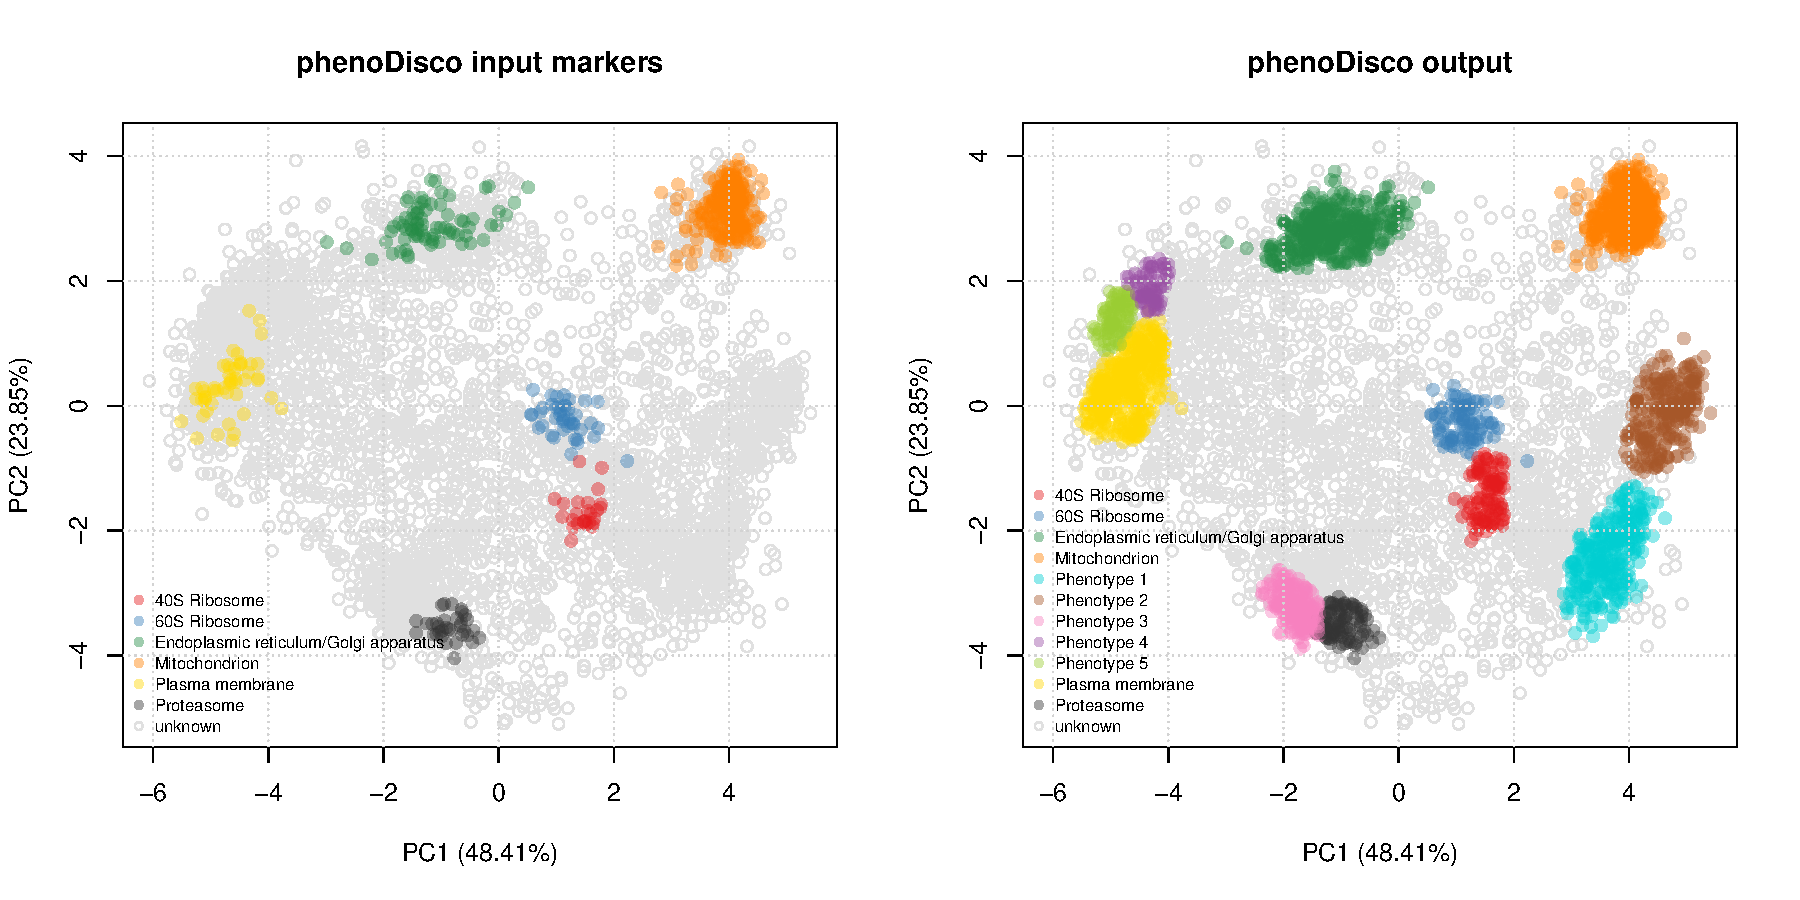
\includegraphics[width=\textwidth]{figure/plotPDres-1} 

\end{knitrout}
  \caption{Results of the novelty detection algorithm.}
  \label{fig:plotPDres}
\end{figure}

We can plot the results using the \texttt{plot2D} function (Figure
\ref{fig:plotPDres}). The five new phenotype data clusters can be
extracted and examined.  In the code chunk below we write the results
to a .csv file using the \texttt{write.exprs} function. We use the
argument \texttt{fDataCols} to specify which columns of the
\texttt{featureData} to write.

\begin{knitrout}
\definecolor{shadecolor}{rgb}{0.969, 0.969, 0.969}\color{fgcolor}\begin{kframe}
\begin{alltt}
\hlkwd{fData}\hlstd{(hl)}\hlopt{$}\hlstd{pd} \hlkwb{<-} \hlkwd{as.character}\hlstd{(}\hlkwd{fData}\hlstd{(hl)}\hlopt{$}\hlstd{pd)}
\hlkwd{write.exprs}\hlstd{(hl,} \hlkwc{fDataCols} \hlstd{=} \hlstr{"pd"}\hlstd{,} \hlkwc{file} \hlstd{=} \hlstr{"pd-results.csv"}\hlstd{,} \hlkwc{sep} \hlstd{=} \hlstr{","}\hlstd{)}
\end{alltt}
\end{kframe}
\end{knitrout}

We can also examine each phenotype interactively and visualise
their protein profiles by using the \texttt{pRolocVis} function in the
\Biocpkg{pRolocGUI} package. We found that phenotype 1 was
enriched in nucleus associated proteins, phenotype 2 in chromatin
associated proteins, phenotype 3 in cytosolic and phenotypes 4 and 5
in lysosomal and endosomal proteins.

% <<vishl, eval=FALSE>>=
% pRolocVis(hl, fcol = "pd")
% @

\section*{Supervised machine learning}

Supervised machine learning, also known as classification, is an
essential tool for the assignment of proteins to distinct sub-cellular
niches. Using a set of labelled training examples i.e. markers, we can
train a machine learning classifier to learn a mapping between the
data i.e. the quantitative protein profiles, and a known localisation.
The trained classifier can then be used to predict the localisation of
a protein of unknown localisation, based on its observed protein
profiles. To date, this method has been extensively used in spatial
quantitative proteomics to assign thousands of proteins to distinct
sub-cellular niches
\cite{hyper,Groen:2014,Trotter:2010,Hall:2009,Dunkley:2006,Tan:2009}.

There are several classification algorithms readily available in
\Biocpkg{pRoloc}, which are documented in the dedicated
\href{http://bioconductor.org/packages/release/bioc/vignettes/pRoloc/inst/doc/pRoloc-ml.pdf}{\Biocpkg{pRoloc}
  machine learning techniques vignette}.  We find the general tendancy
to be that it is not the choice of classifier, but the improper
optimisation of the algorithmic parameters, that limits classification
accuracy. Before employing any classification algorithm and generating
a model on the training data, one must first find the optimal
parameters for the algorithm of choice.

\subsection*{Optimisation}

In the code chunk below we use a Support Vector Machine (SVM) to learn
a classifier on the labelled training data. As previously mentioned,
one first needs to train the classifiers parameters before an
algorithm can be used to predict the class labels of the proteins with
unknown location. One of the most common ways to optimise the
parameters of a classifier is to partition the labelled data into
training and testing subsets. In this framework parameters are tested
via a grid search using cross-validation on the training
partition. The best parameters chosen from the cross-validation stage
are then used to build a classifier to predict the class labels of the
protein profiles on the test partition. Observed and expected
classication results can be compared, and then used to assess how well
a given model works by getting an estimate of the classiers ability to
achieve a good generalisation i.e. that is given an unknown example
predict its class label with high accuracy. In \Biocpkg{pRoloc},
algorithmic performance is estimated using stratified 80/20
partitioning for the training/testing subsets respectively, in
conjuction with five-fold cross-validation in order to optimise the
free parameters via a grid search. This procedure is usually repeated
100 times and then the best parameter(s) are selected upon
investigation of classifier accuracy. We recommend a minimum of 13
markers per sub-cellular class for stratified 80/20 partitioning and
5-fold cross-validation; this allows a minimum of 10 examples for
parameter optimisation on the training partition i.e. 2 per fold for
5-fold cross-validation, and then 3 for testing the best parameters on
the validation set.

Classifier accuracy is estimated using the macro F1 score, i.e. the
harmonic mean of precision and recall. In the code chunk below we
demonstrate how to optimise the free parameters, \texttt{sigma} and
\texttt{cost}, of a classical SVM classifier with a Gaussian kernel
using the function \texttt{svmOptimisation}. As the number of labelled
instances per class varies from organelle to organelle, we can account
for class imbalance by setting specific class weights when generating
the SVM model. Below the weights, \texttt{w} are set to be inversely
proportional to the class frequencies.



\begin{knitrout}
\definecolor{shadecolor}{rgb}{0.969, 0.969, 0.969}\color{fgcolor}\begin{kframe}
\begin{alltt}
\hlstd{w} \hlkwb{<-} \hlkwd{table}\hlstd{(}\hlkwd{getMarkers}\hlstd{(hl,} \hlkwc{verbose} \hlstd{=} \hlnum{TRUE}\hlstd{))}
\end{alltt}
\begin{verbatim}
## organelleMarkers
##            40S Ribosome            60S Ribosome      Actin cytoskeleton 
##                      27                      43                      13 
##                 Cytosol   Endoplasmic reticulum                Endosome 
##                      43                      95                      12 
##    Extracellular matrix                Lysosome           Mitochondrion 
##                      10                      33                     383 
##     Nucleus - Chromatin Nucleus - Non-chromatin              Peroxisome 
##                      64                      85                      17 
##         Plasma membrane              Proteasome                 unknown 
##                      51                      34                    4122
\end{verbatim}
\begin{alltt}
\hlstd{w} \hlkwb{<-} \hlnum{1}\hlopt{/}\hlstd{w[}\hlkwd{names}\hlstd{(w)} \hlopt{!=} \hlstr{"unknown"}\hlstd{]}
\end{alltt}
\end{kframe}
\end{knitrout}

\begin{knitrout}
\definecolor{shadecolor}{rgb}{0.969, 0.969, 0.969}\color{fgcolor}\begin{kframe}
\begin{alltt}
\hlcom{## 100 rounds of optimisation with five-fold cross-validation}
\hlstd{params} \hlkwb{<-} \hlkwd{svmOptimisation}\hlstd{(hl,} \hlkwc{fcol} \hlstd{=} \hlstr{"markers"}\hlstd{,}
                          \hlkwc{times} \hlstd{=} \hlnum{100}\hlstd{,} \hlkwc{xval} \hlstd{=} \hlnum{5}\hlstd{,}
                          \hlkwc{class.weights} \hlstd{= w)}
\end{alltt}
\end{kframe}
\end{knitrout}

As mentioned previously, we rely on the default feature variable
\texttt{"markers"} to define the class labels and hence do not need to
specify it in the above code chunk.  To use another feature variables,
one need to explicitly specify its name using the \texttt{fcol}
argument (for example \texttt{fcol = "markers2"}).

The output \texttt{params} is an object of class \texttt{GenRegRes}; a
dedicated container for the storage of the design and results from a
machine learning optimisation. To assess classifier performance we can
examine the macro F1 scores and the most frequently chosen
parameters. A high macro F1 score indicates that the marker proteins
in the test dataset are consistently and correctly assigned by the the
algorithm. Often more than one parameter or set of parameters gives
rise to the best generalisation accuracy. As such it is always
important to investigate the model parameters and critically assess
the best choice. The \texttt{f1Count} function counts the number of
parameter occurences above a certain F1 value. The best choice may not
be as simple as the parameter set that gives rise to the highest macro
F1 score. One must be careful to avoid overfitting, and choose
parameters that frequently provide high classification
accuracy. Below, we see that only a sigma of 0.1 produces macro F1
scores above 0.6, but that a cost of 16 is much more frequently chosen
than lower values.

\begin{knitrout}
\definecolor{shadecolor}{rgb}{0.969, 0.969, 0.969}\color{fgcolor}\begin{kframe}
\begin{alltt}
\hlkwd{f1Count}\hlstd{(params,} \hlnum{0.6}\hlstd{)}
\end{alltt}
\begin{verbatim}
##     4  8 16
## 0.1 1 10 89
\end{verbatim}
\end{kframe}
\end{knitrout}

The parameter optimistion results can also be visualised as a boxplot
or heatmap, as shown in figure \ref{fig:visualisOptHide}.  The
\texttt{plot} method for \texttt{GenRegRes} object shows the
respective distributions of the 100 macro F1 scores for the best
cost/sigma parameter pairs, and \texttt{levelPlot} shows the averaged
macro F1 scores, for the full range of parameter values. These figures
also indicate that values of 0.1 and 16 for sigma and cost
consistently deliver better classification scores. 

\begin{knitrout}
\definecolor{shadecolor}{rgb}{0.969, 0.969, 0.969}\color{fgcolor}\begin{kframe}
\begin{alltt}
\hlkwd{plot}\hlstd{(params)}
\hlkwd{levelPlot}\hlstd{(params)}
\end{alltt}
\end{kframe}
\end{knitrout}

\begin{figure}[!ht]
  \centering
\begin{knitrout}
\definecolor{shadecolor}{rgb}{0.969, 0.969, 0.969}\color{fgcolor}
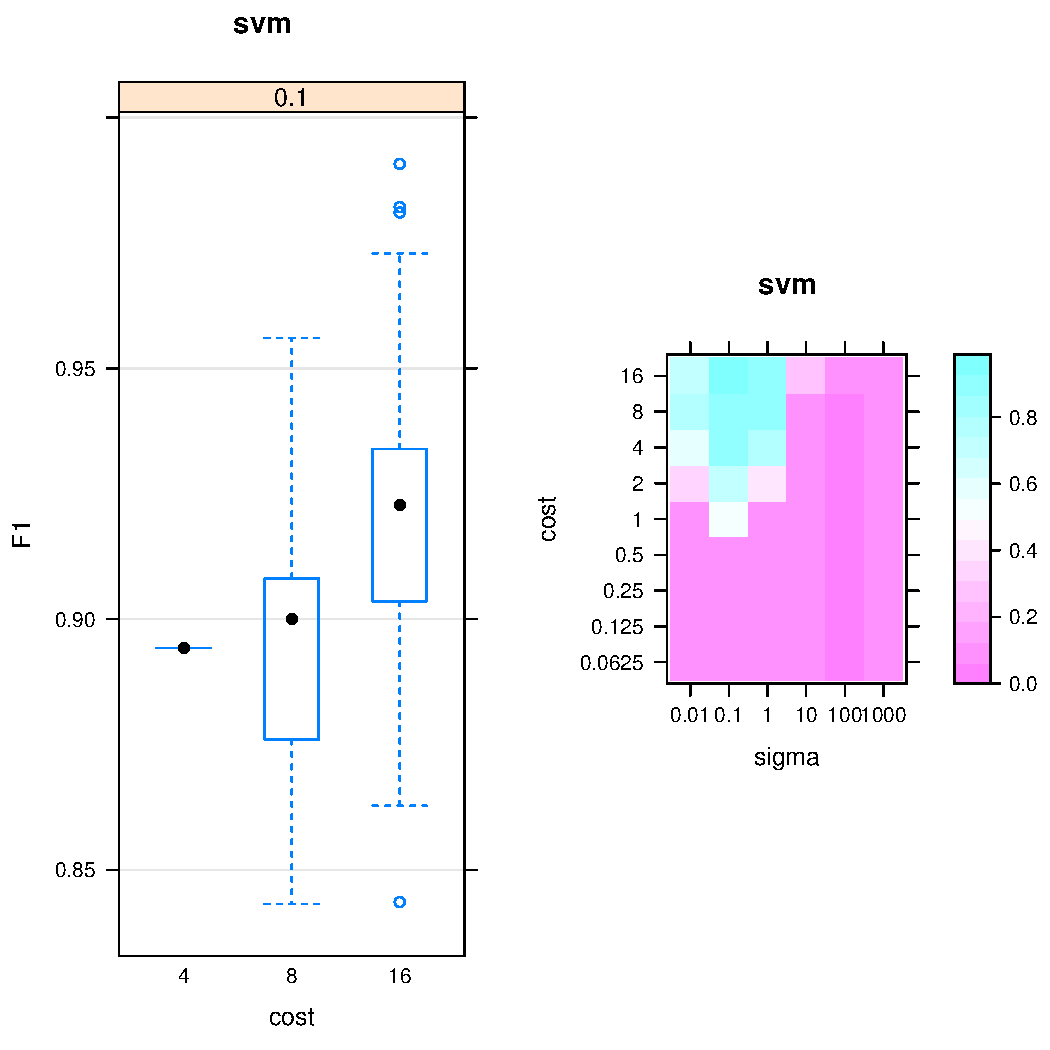
\includegraphics[width=.65\textwidth]{figure/visualiseOptHide-1} 

\end{knitrout}
  \caption{Assessment of the classification model parameter optimisation.}
  \label{fig:visualisOptHide}
\end{figure}


By using the function \texttt{getParams} we can extract the best set
of parameters. Currently, \texttt{getParams} retrieves the first best
set automatically, but users are encouraged to critically assess
whether this is the most wise choice (which it is, as demonstrated
above).

\begin{knitrout}
\definecolor{shadecolor}{rgb}{0.969, 0.969, 0.969}\color{fgcolor}\begin{kframe}
\begin{alltt}
\hlstd{(best} \hlkwb{<-} \hlkwd{getParams}\hlstd{(params))}
\end{alltt}
\begin{verbatim}
## sigma  cost 
##   0.1  16.0
\end{verbatim}
\end{kframe}
\end{knitrout}

Once we have selected the best parameters we can then use them to
build a classifier from the labelled marker proteins.


\subsection*{Classification}

We can use the function \texttt{svmClassification} to return a
classification result for all unlabelled instances in the dataset
corresponding to their most likely sub-cellular location. The
algorithm parameters are passed to the function, along with the class
weights. As above, the \texttt{fcol} argument does not need to be
specified as we use the labels defined in the default
\texttt{"markers"} feature variable.

\begin{knitrout}
\definecolor{shadecolor}{rgb}{0.969, 0.969, 0.969}\color{fgcolor}\begin{kframe}
\begin{alltt}
\hlstd{hl} \hlkwb{<-} \hlkwd{svmClassification}\hlstd{(hl, params,} \hlkwc{class.weights} \hlstd{= w,} \hlkwc{fcol} \hlstd{=} \hlstr{"markers"}\hlstd{)}
\end{alltt}
\end{kframe}
\end{knitrout}

Automatically, the output of the above classification, the organelle
predictions and assignment scores, are stored in the
\texttt{featureData} slot of the \texttt{MSnSet}. In this case, they
are given the labels \texttt{svm} and \texttt{svm.scores} for the
predictions and scores respectively. The resultant predictions can be
visualised using \texttt{plot2D}. In the code chunk below
\texttt{plot2D} is called to generate a PCA plot of the data and
\texttt{fcol} is used to specify where the new assignments are located
e.g. \texttt{fcol = "svm"}.

Additionally, when calling \texttt{plot2D} we can use the \texttt{cex}
argument to change the size of each point on the plot to be inversely
proportional to the SVM score. This gives an initial overview of the
high scoring localisations from the SVM predictions.



\begin{figure}[!ht]
  \centering
\begin{knitrout}
\definecolor{shadecolor}{rgb}{0.969, 0.969, 0.969}\color{fgcolor}\begin{kframe}
\begin{alltt}
\hlcom{## set point size of each protein to be inversely proportional to the}
\hlstd{ptsze} \hlkwb{<-} \hlkwd{exp}\hlstd{(}\hlkwd{fData}\hlstd{(hl)}\hlopt{$}\hlstd{svm.scores)} \hlopt{-} \hlnum{1}
\hlcom{## plot new predictions}
\hlkwd{plot2D}\hlstd{(hl,} \hlkwc{fcol} \hlstd{=} \hlstr{"svm"}\hlstd{,} \hlkwc{cex} \hlstd{= ptsze)}
\hlkwd{addLegend}\hlstd{(hl,} \hlkwc{fcol} \hlstd{=} \hlstr{"svm"}\hlstd{,} \hlkwc{where} \hlstd{=} \hlstr{"bottomleft"}\hlstd{,} \hlkwc{bty} \hlstd{=} \hlstr{"n"}\hlstd{,} \hlkwc{cex} \hlstd{=} \hlnum{.5}\hlstd{)}
\end{alltt}
\end{kframe}
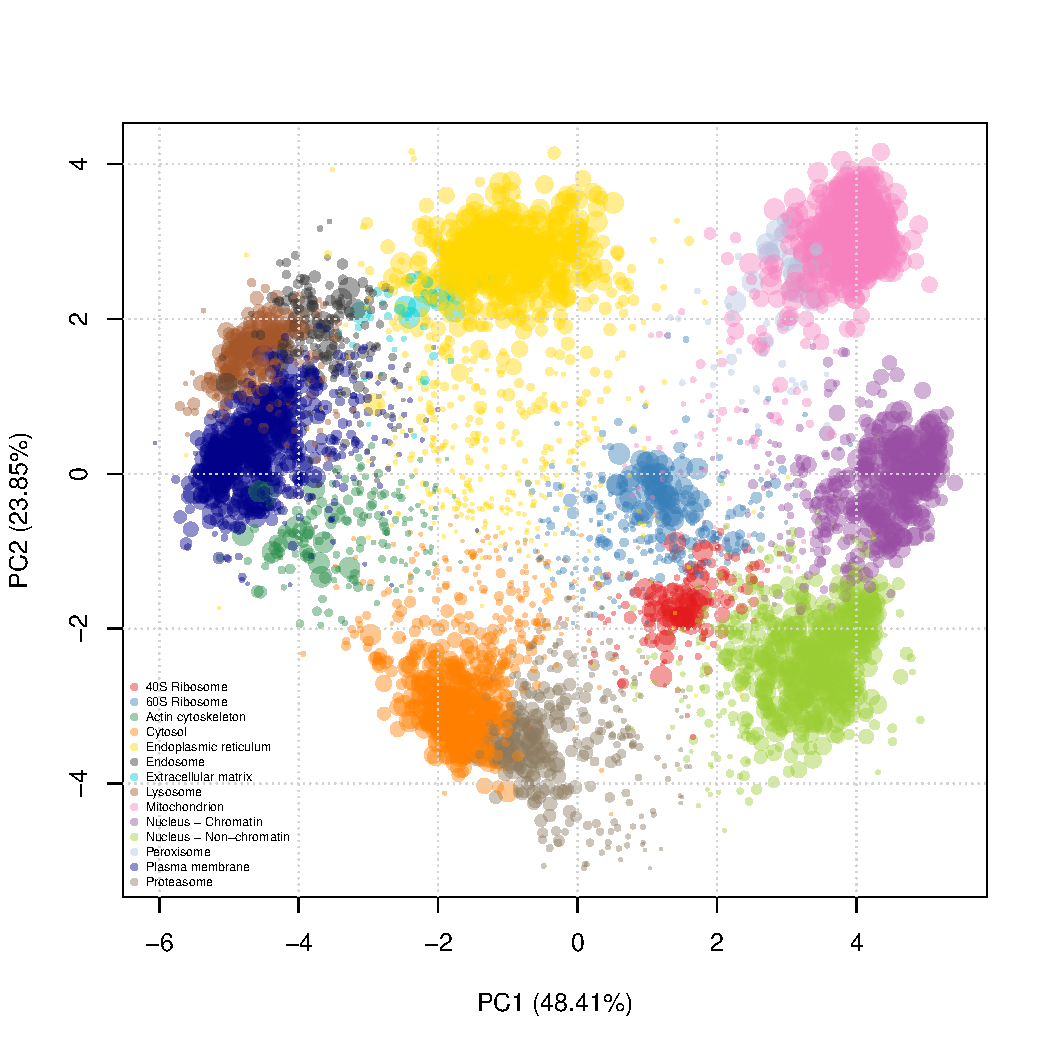
\includegraphics[width=.8\textwidth]{figure/plotSVM-1} 

\end{knitrout}
\caption{Classification results. Colours indicate class membership and
  point size are representative or the classification confidence.}
  \label{fig:plotSVM}
\end{figure}


The adjustment of the point size intuitively confers important
information that is more difficult to define formally (we
will address in the next section). The classifier (SVM in our case, but
this is also valid of other classifiers) defines boundaries based on
the labelled marker proteins. These class/organelle boundaries define
how non-assigned proteins are classified and with what confidence.

\subsection*{Thresholding}\label{sec:thresholding}

It is common when applying a supervised classification algorithm to
set a specific score cutoff on which to define new assignments, below
which classifications are kept unknown/unassigned. This is important
as in a supervised learning setup, proteins can only be predicted to
be localised to one of the sub-cellular niches that appear in the
labelled training data. We can not guarantee (and do not expect) that
the whole sub-cellular diversity to be represented in the labelled
training data as (1) finding markers that represent the whole
diversity of the cell is challenging (especially obtaining dual- and
multiply-localised protein markers) and (2) many sub-cellular niches
contain too few proteins to train on (see above for a motivation of a
minimum of 13 markers).

Deciding on a threshold is not trivial as classifier scores are
heavily dependent upon the classifier used and different sub-cellular
niches can exhibit different score distributions, as highlighted in
the boxplot below. We recommend users to set class-specific
thresholds.  In the code chunk below we display a boxplot of the score
distributions per organelle (Figure \ref{fig:threshold}). 

\begin{figure}[!ht]
  \centering
\begin{knitrout}
\definecolor{shadecolor}{rgb}{0.969, 0.969, 0.969}\color{fgcolor}\begin{kframe}
\begin{alltt}
\hlcom{## First remove the markers}
\hlstd{preds} \hlkwb{<-} \hlkwd{unknownMSnSet}\hlstd{(hl)}
\hlcom{## Plot a boxplot of the scores of each organelle}
\hlkwd{par}\hlstd{(}\hlkwc{oma} \hlstd{=} \hlkwd{c}\hlstd{(}\hlnum{10.5}\hlstd{,} \hlnum{0}\hlstd{,} \hlnum{0}\hlstd{,} \hlnum{0}\hlstd{))}
\hlkwd{boxplot}\hlstd{(svm.scores} \hlopt{~} \hlstd{svm,} \hlkwc{data} \hlstd{=} \hlkwd{fData}\hlstd{(preds),}
        \hlkwc{ylab} \hlstd{=} \hlstr{"SVM scores"}\hlstd{,} \hlkwc{las} \hlstd{=} \hlnum{2}\hlstd{)}
\end{alltt}
\end{kframe}
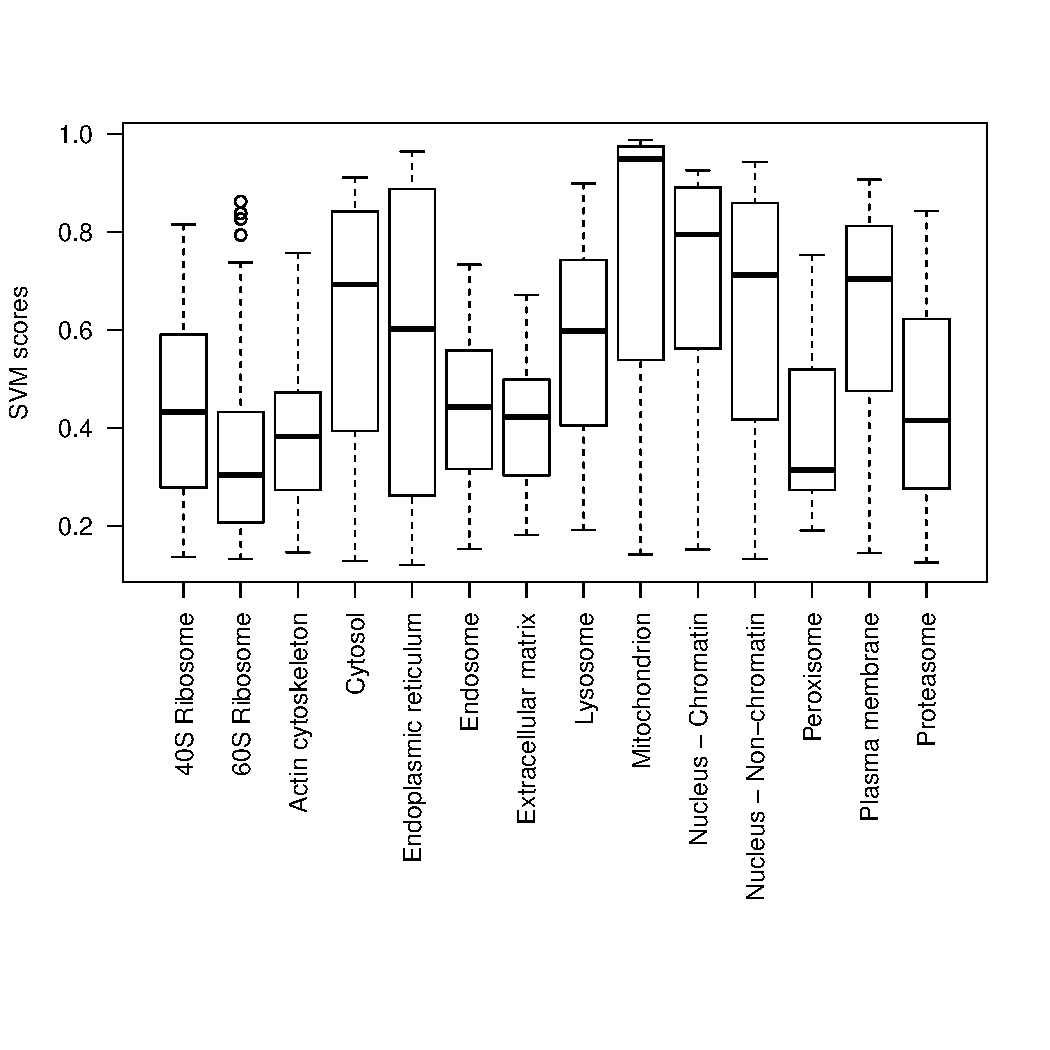
\includegraphics[width=.8\textwidth]{figure/thresholds-1} 

\end{knitrout}
  \caption{Visualistion of class-specific classification score distribution.}
  \label{fig:threshold}
\end{figure}

There are many ways to set thresholds and the choice of method will
depend on the biological question and experimental design at hand. One
viable approach in the frame of the above experimetal design would be
to manually set a FDR, say 5\%, per organelle. To do this the user
would examine the top scoring predictions for each organelle, and then
set a threshold at the score at which they achieve 5\% of false
assignments per organelle.  The definintion of a false assignment
would depend on the information available, for example, validity or
lack of validity for the localisation from another experiment as
reported in the literature or a reliable database.  If such
information is not available, one crude method is to set a threshold
per organelle by extracting the median or 3rd quantile score per
organelle.  For example, in the code chunk below, we use the
\texttt{orgQuants} function to extract the median organelle scores and
then pass these scores to the \texttt{getPredictions} function to
extract the new localisations that meet this scoring criteria. Any
sub-cellular predictions that fall below the specified thresholds are
labelled as unknown.

\begin{knitrout}
\definecolor{shadecolor}{rgb}{0.969, 0.969, 0.969}\color{fgcolor}\begin{kframe}
\begin{alltt}
\hlstd{ts} \hlkwb{<-} \hlkwd{orgQuants}\hlstd{(hl,} \hlkwc{fcol} \hlstd{=} \hlstr{"svm"}\hlstd{,} \hlkwc{scol} \hlstd{=} \hlstr{"svm.scores"}\hlstd{,} \hlkwc{mcol} \hlstd{=} \hlstr{"markers"}\hlstd{,} \hlkwc{t} \hlstd{=} \hlnum{.5}\hlstd{)}
\end{alltt}
\begin{verbatim}
##            40S Ribosome            60S Ribosome      Actin cytoskeleton 
##               0.4368179               0.3037653               0.3856993 
##                 Cytosol   Endoplasmic reticulum                Endosome 
##               0.6916475               0.5951696               0.4377555 
##    Extracellular matrix                Lysosome           Mitochondrion 
##               0.4317514               0.5919750               0.9527663 
##     Nucleus - Chromatin Nucleus - Non-chromatin              Peroxisome 
##               0.7947663               0.7096575               0.3269003 
##         Plasma membrane              Proteasome 
##               0.7210996               0.4155492
\end{verbatim}
\begin{alltt}
\hlstd{hl} \hlkwb{<-} \hlkwd{getPredictions}\hlstd{(hl,} \hlkwc{fcol} \hlstd{=} \hlstr{"svm"}\hlstd{,} \hlkwc{scol} \hlstd{=} \hlstr{"svm.scores"}\hlstd{,} \hlkwc{mcol} \hlstd{=} \hlstr{"markers"}\hlstd{,} \hlkwc{t} \hlstd{= ts)}
\end{alltt}
\begin{verbatim}
## ans
##            40S Ribosome            60S Ribosome      Actin cytoskeleton 
##                      85                     172                      88 
##                 Cytosol   Endoplasmic reticulum                Endosome 
##                     296                     477                     100 
##    Extracellular matrix                Lysosome           Mitochondrion 
##                      27                     123                     513 
##     Nucleus - Chromatin Nucleus - Non-chromatin              Peroxisome 
##                     231                     344                      42 
##         Plasma membrane              Proteasome                 unknown 
##                     318                     157                    2059
\end{verbatim}
\end{kframe}
\end{knitrout}

The output of \texttt{getPredictons} is the original \texttt{MSnSet}
dataset with a new feature variable appended to the feature data
called \texttt{fcol.pred} (i.e. in our case \texttt{svm.pred})
containing the prediction results. The results can also be visualied
using \texttt{plot2D} function (Figure \ref{fig:plotres}) and
extracted by retrieving that specific column from the feature metadata
using, for example, \texttt{fData(hl)\$svm.pred}.



\begin{figure}[!ht]
    \centering
\begin{knitrout}
\definecolor{shadecolor}{rgb}{0.969, 0.969, 0.969}\color{fgcolor}\begin{kframe}
\begin{alltt}
\hlkwd{plot2D}\hlstd{(hl,} \hlkwc{fcol} \hlstd{=} \hlstr{"svm.pred"}\hlstd{)}
\end{alltt}
\end{kframe}
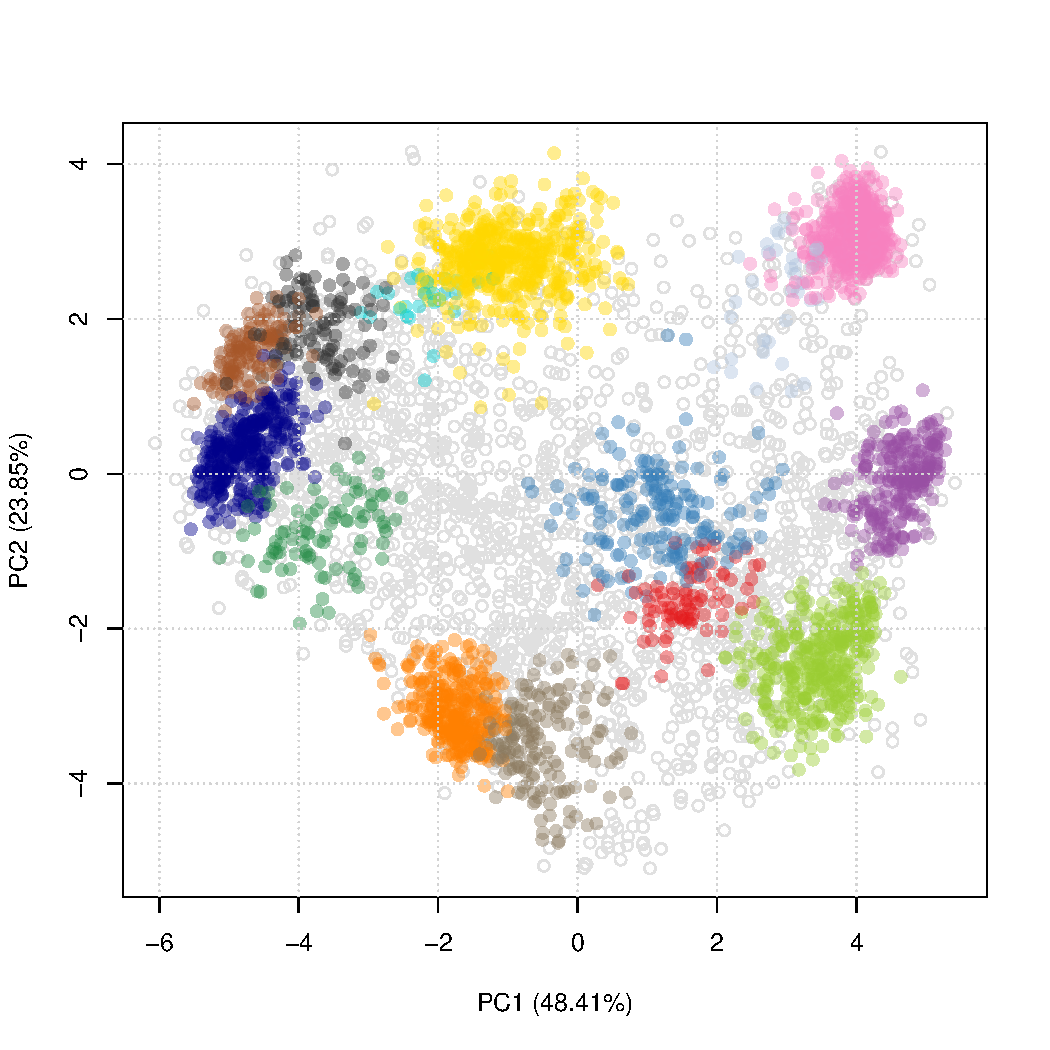
\includegraphics[width=.7\textwidth]{figure/plotres-1} 

\end{knitrout}
  \caption{Results of the localisation preductions after thresholding.}
  \label{fig:plotres}
\end{figure}


There is also a dedicated interactive application to help users
examine these distributions in the \Biocpkg{pRolocGUI} package (Figure
\ref{fig:classifyapp}).  This app can be launched via the
\texttt{pRolocVis} function and specifying the argument \texttt{app =
  "classify"} along with the relevent \texttt{fcol}, \texttt{scol} and
\texttt{mcol} which refer to the columns in the feature data that
contain the new assignments, assignment scores and markers
respectively (see also \texttt{fvarLabels(svmres)}).

\begin{knitrout}
\definecolor{shadecolor}{rgb}{0.969, 0.969, 0.969}\color{fgcolor}\begin{kframe}
\begin{alltt}
\hlkwd{library}\hlstd{(}\hlstr{"pRolocGUI"}\hlstd{)}
\hlkwd{pRolocVis}\hlstd{(hl,} \hlkwc{app} \hlstd{=} \hlstr{"classify"}\hlstd{,} \hlkwc{fcol} \hlstd{=} \hlstr{"svm"}\hlstd{,} \hlkwc{scol} \hlstd{=} \hlstr{"svm.scores"}\hlstd{,} \hlkwc{mcol} \hlstd{=} \hlstr{"markers"}\hlstd{)}
\end{alltt}
\end{kframe}
\end{knitrout}

\begin{figure}[!ht]
  \centering
  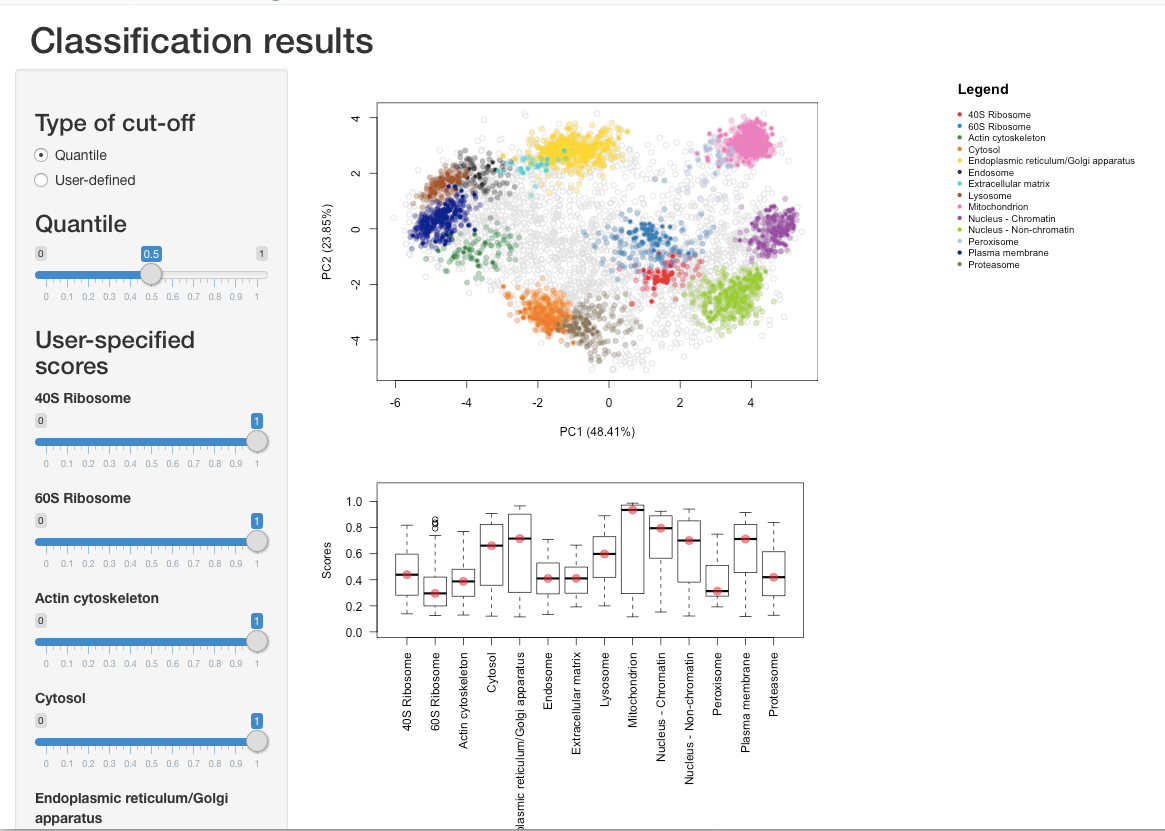
\includegraphics[width=0.7\textwidth]{./Figures/classify.png}
  \caption{The classify application enable the interactive exploration
    of classification score thresholding.}
  \label{fig:classifyapp}
\end{figure}


The data is loaded and displayed on a PCA plot and a boxplot is used
to display the classifier scores by data class. On the left, there is
a sidebar panel with sliders to control the thresholds upon which
classifications are made. There are two types of cut-off that the user
can choose from: (1) \textit{Quantile} and (2)
\textit{User-defined}. By default, when the application is launched
quatile scoring is selected and set to 0.5, the median. The
class-specific score thresholds that correspond to selecting the
desired quantile are shown on as red dots on the boxplot. The
assignments on the PCA plot are also updated according to the selected
threshold. The quantile threshold can be set by moving the
corresponding quantile slider. If one wished to set their own cut-offs
the \textit{User-defined} radio button must be selected and then the
sliders for defining user-specified scores become active and the
scores and highlighted on the boxplot by blue dots. For more
information we refer users to the \Biocpkg{pRolocGUI} tutorial
\href{http://bioconductor.org/packages/release/bioc/vignettes/pRolocGUI/inst/doc/pRolocGUI.html}{vignette}.

\clearpage

\section*{Transfer learning}

In addition to high quality MS-based quantitative proteomics data,
there exist a number of other sources of information that are freely
available in the public domain that may be useful to assign a protein
to its sub-cellular niche. For example, imaging from
immunofluorescence microscopy, protein annotations and sequences, and
protein-protein interactions among others, represent a rich and vast
source of complementary information. We can integrate this auxiliary
information with our primary MS-based quantitative data using a
paradigm known as transfer learning (TL). The integration of data
between different technologies is one of the biggest challenges in
computational biology to date and the \Biocpkg{pRoloc} package
provides functionality to do such analyses. We recently developed two
transfer learning algorithms using a $k$-NN and SVM framework and
applied them to the task of protein localisation prediction
\cite{Breckels:2016}. In this section we will begin with explaining
the concept of transfer learning and then show how to apply this in
the frame of spatial proteomics and protein localisation prediction.

In TL one typically has a primary task that one wishes to solve, and
some complementary (often heterogeneous) auxiliary information that is
related to the primary learning objective, that can be used to help
solve the primary goal. For example, here our primary task is to
assign proteins to their sub-cellular niche with high generalisation
accuracy from data collected from quantitative MS-based experiments.
We have already seen that straightforward supervised ML works well for
these types of experiments, however, Transfer learning is particularly
useful for classes that are not as well separated.

In the example below we extract Gene Ontology (GO) information to use
as an auxiliary data source to help solve our task of protein
localisation prediction.

Using the functions \texttt{setAnnotationParams} and
\texttt{makeGoSet} we can contruct an auxiliary \texttt{MSnSet} of GO
terms, from the primary data's features i.e. the protein accession
numbers. All the GO terms associated to each accession number are
retrieved and used to create a binary matrix where a 1 (0) at position
$(i, j)$ indicates that term $j$ has (not) been used to annotate
protein $i$. The GO terms are retrieved from an appropriate repository
using the \Biocpkg{biomaRt} package. The specific Biomart repository
and query will depend on the species under study and the type of
identifiers. The first step is to construct the annotation parameters
that will enable to perform the query, which is done using
\texttt{setAnnotationParams}. Typing into the R console \texttt{par <-
  setAnnotationParams()} will present two menus, firstly asking you to
identify the species of study, and then what type of identifier you
have used to annotate the proteins in your \texttt{MSnSet}. It is also
possible to pass patterns to match the species e.g. in the code chunk
below we pass \texttt{"Mus musculus"}, and the identifier type for our
data (see \texttt{featureNames(hl)}) which is
\texttt{"Uniprot/Swissprot"}, for the Biomart query.

\begin{knitrout}
\definecolor{shadecolor}{rgb}{0.969, 0.969, 0.969}\color{fgcolor}\begin{kframe}
\begin{alltt}
\hlstd{par} \hlkwb{<-} \hlkwd{setAnnotationParams}\hlstd{(}\hlkwc{inputs} \hlstd{=} \hlkwd{c}\hlstd{(}\hlstr{"Mus musculus"}\hlstd{,} \hlstr{"UniProt/Swissprot"}\hlstd{))}
\end{alltt}
\end{kframe}
\end{knitrout}

Now we have contructed the query parameters we can use the
\texttt{makeGoSet} function to retrieve and build an auxiliary GO
\texttt{MSnSet} as described above. By default, the cellular component
terms are downloaded, without any filtering on evidence codes. It is
also possible to download terms from the molecular function and
biological process GO namespaces, and also apply filtering based on
evidence codes as desired, see \texttt{?makeGoSet} for more details.

\begin{knitrout}
\definecolor{shadecolor}{rgb}{0.969, 0.969, 0.969}\color{fgcolor}\begin{kframe}
\begin{alltt}
\hlstd{gocc} \hlkwb{<-} \hlkwd{makeGoSet}\hlstd{(hl,} \hlkwc{params} \hlstd{= par,} \hlkwc{namespace} \hlstd{=} \hlstr{"cellular_component"}\hlstd{)}
\end{alltt}
\end{kframe}
\end{knitrout}

The function \texttt{makeGoSet} uses the \Biocpkg{biomaRt} package to
query the relevent database (e.g. Ensembl, Uniprot) for GO terms. All
GO terms that have been observed for the 5032 proteins in the
hyperLOPIT dataset are retieved. Users should note that the number of
GO terms retreived is also dependent on the database version queried
and thus is always subject to change. We find it is common to see GO
terms with only one protein assigned to that term. Such terms do not
bring any information for building the classifier and are thus removes
using the \texttt{filterBinMSnSet} function.

\begin{knitrout}
\definecolor{shadecolor}{rgb}{0.969, 0.969, 0.969}\color{fgcolor}\begin{kframe}
\begin{alltt}
\hlstd{gocc} \hlkwb{<-} \hlkwd{filterBinMSnSet}\hlstd{(hl)}
\end{alltt}
\end{kframe}
\end{knitrout}

Now that we have generated our auxiliary data, we can use the
\textit{k}-NN implementation of transfer learning available in
\Biocpkg{pRoloc} to integrate this with our primary MS-based
quantitative proteomics data using the functions
\texttt{knntlOptimisation} to estimate the free-parameters for the
integration, and \texttt{knntlClassification} to do the
predictions. We have shown that using transfer learning results in the
assignment of proteins to sub-cellular niches with a higher
generalisation accuracy than using standard supervised machine
learning with a single source of information \cite{Breckels:2016}.

\subsection*{TL optimisation}

The first step, as with any machine learning algorithm, is to optimise
any free paramaters of the classifier. For the $k$-NN TL classifier
there are two sets of parameters that need optimising: the first set
are the $k$'s for the primary and auxiliary data sources required for
the nearest neighbour calculations for each data source. The second
set of parameters (noted by a vector of $\theta$ weights) that require
optimising are the class weights, one per subcellular niche, that
control the proportion of primary and auxiliary data to use for
learning. A weight can take any real value number between 0 and 1. A
weight of $\theta = 1$ indicates that all weight is given to the
primary data (and this implicitly implies that a weight of
$1 - \theta = 0$ is given to the auxiliary data), and similarly a
weight of $\theta = 0$ implies that all weight is given to the
auxiliary data (so 0 is given to the primary source). If we conduct a
parameter seach and test weights $\theta = {0, 1/3, 2/3, 1}$ for each
class, and if we have, for example 10 subcellular niches, this will
result in \texttt{4$^{10}$} different combinations of parameters to
test. The parameter optimisation is therefore time consuming and as
such we recommend making use of a computing cluster (code and
submissing scripts are also available in the supporting
information). The markers in the \texttt{hl} dataset contain 14
subcellular classes. If we examine these markers and classes on the
PCA plot above we can see that in particular the two ribosomes and two
nuclear compartments are highly separated along the first two
components, this is also evident from the profiles plot which gives us
a good indication that these subcellular niches are well-resolved in
the hyperLOPIT dataset. Transfer learning is particularly useful for
classes that are not as well separated. We find that subcellular
niches that are well-separated under hyperLOPIT and LOPIT obtain a
class score of 1 (i.e. use only primary data from transfer learning
\cite{Breckels:2016}). Therefore, for the optimisation stage of the
analyses we can already infer a subcellular class weight of 1 for
these niches and only optimise over the remaining organelles.  This
can signifciantly cut down optimisation time as by removing these 4
classes from the optimisation (and not the classification) we only
have \texttt{4$^{10}$} class weight combinations to consider instead
of \texttt{4$^{14}$} combinations.

In the example below we remove these 4 classes from the marker set,
re-run the \texttt{knnOptimisation} for each data source and then run
the \texttt{knntlOptimisation} with the 10 remaining classes. (Note:
this is not run live as this the \texttt{hl} dataset with 10 classes,
707 markers and 4$^{10}$ combinations of parameters takes around 76
hours to run on the University of Cambridge HPC using 256 workers).

To remove the 4 classes and create a new column of markers in the
feature data called \texttt{tlmarkers} to use for the analysis:



\begin{knitrout}
\definecolor{shadecolor}{rgb}{0.969, 0.969, 0.969}\color{fgcolor}\begin{kframe}
\begin{alltt}
\hlcom{## create new markers column for tl markers}
\hlkwd{fData}\hlstd{(hl)}\hlopt{$}\hlstd{tlmarkers} \hlkwb{<-} \hlkwd{fData}\hlstd{(hl)}\hlopt{$}\hlstd{markers}
\hlkwd{fData}\hlstd{(gocc)}\hlopt{$}\hlstd{tlmarkers} \hlkwb{<-} \hlkwd{fData}\hlstd{(gocc)}\hlopt{$}\hlstd{markers}

\hlcom{## Remove 4 classes}
\hlstd{torm}  \hlkwb{<-} \hlkwd{c}\hlstd{(}\hlstr{"40S Ribosome"}\hlstd{,} \hlstr{"60S Ribosome"}\hlstd{,}
           \hlstr{"Nucleus - Chromatin"}\hlstd{,}
           \hlstr{"Nucleus - Non-chromatin"}\hlstd{)}
\hlkwa{for} \hlstd{(i} \hlkwa{in} \hlkwd{seq}\hlstd{(torm)) \{}
  \hlstd{hl} \hlkwb{<-} \hlkwd{fDataToUnknown}\hlstd{(hl,} \hlkwc{from} \hlstd{= torm[i],} \hlkwc{fcol} \hlstd{=} \hlstr{"tlmarkers"}\hlstd{)}
  \hlstd{gocc} \hlkwb{<-} \hlkwd{fDataToUnknown}\hlstd{(gocc,} \hlkwc{from} \hlstd{= torm[i],} \hlkwc{fcol} \hlstd{=} \hlstr{"tlmarkers"}\hlstd{)}
\hlstd{\}}
\hlkwd{getMarkerClasses}\hlstd{(hl,} \hlkwc{fcol} \hlstd{=} \hlstr{"tlmarkers"}\hlstd{)}
\end{alltt}
\begin{verbatim}
##  [1] "Actin cytoskeleton"    "Cytosol"              
##  [3] "Endoplasmic reticulum" "Endosome"             
##  [5] "Extracellular matrix"  "Lysosome"             
##  [7] "Mitochondrion"         "Peroxisome"           
##  [9] "Plasma membrane"       "Proteasome"
\end{verbatim}
\begin{alltt}
\hlkwd{getMarkerClasses}\hlstd{(gocc,} \hlkwc{fcol} \hlstd{=} \hlstr{"tlmarkers"}\hlstd{)}
\end{alltt}
\begin{verbatim}
##  [1] "Actin cytoskeleton"    "Cytosol"              
##  [3] "Endoplasmic reticulum" "Endosome"             
##  [5] "Extracellular matrix"  "Lysosome"             
##  [7] "Mitochondrion"         "Peroxisome"           
##  [9] "Plasma membrane"       "Proteasome"
\end{verbatim}
\end{kframe}
\end{knitrout}

\paragraph{TL optimisation stage 1} Run \texttt{knnOptimisation} to get
the best $k$'s for each data source.

\begin{knitrout}
\definecolor{shadecolor}{rgb}{0.969, 0.969, 0.969}\color{fgcolor}\begin{kframe}
\begin{alltt}
\hlcom{## get best k's}
\hlstd{kpopt} \hlkwb{<-} \hlkwd{knnOptimisation}\hlstd{(hl,} \hlkwc{fcol} \hlstd{=} \hlstr{"tlmarkers"}\hlstd{)}
\hlstd{kaopt} \hlkwb{<-} \hlkwd{knnOptimisation}\hlstd{(gocc,} \hlkwc{fcol} \hlstd{=} \hlstr{"tlmarkers"}\hlstd{)}
\end{alltt}
\end{kframe}
\end{knitrout}

From examining the parameter seach plots as described in section
\textit{Optimisation}, we find the best $k$'s for both the primary and
auxiliary are 3.

\paragraph{TL optimisation stage 2} Run \texttt{knntlOptimisation} to
get the best transfer learning weights for each sub-cellular class.

\begin{knitrout}
\definecolor{shadecolor}{rgb}{0.969, 0.969, 0.969}\color{fgcolor}\begin{kframe}
\begin{alltt}
\hlcom{## Set appropriate parallelisation backend and  }
\hlcom{## number of workers for the tl}
\hlstd{par} \hlkwb{<-} \hlkwd{SnowParam}\hlstd{(}\hlnum{255L}\hlstd{,} \hlkwc{type} \hlstd{=} \hlstr{"MPI"}\hlstd{)}

\hlcom{## Now peform tl optimisation }
\hlstd{tlopt} \hlkwb{<-} \hlkwd{knntlOptimisation}\hlstd{(hl, gocc,} \hlkwc{fcol} \hlstd{=} \hlstr{"tlmarkers"}\hlstd{,}
                           \hlkwc{length.out} \hlstd{=} \hlnum{4}\hlstd{,} \hlkwc{times} \hlstd{=} \hlnum{50}\hlstd{,}
                           \hlkwc{xval} \hlstd{=} \hlnum{5}\hlstd{,} \hlkwc{k} \hlstd{=} \hlkwd{c}\hlstd{(}\hlnum{3}\hlstd{,} \hlnum{3}\hlstd{),}
                           \hlkwc{BPPARAM} \hlstd{= par)}
\end{alltt}
\end{kframe}
\end{knitrout}

The results of the optimisation can be visalised using the
\texttt{plot} method for \texttt{tlopt} optimisation result:



\begin{figure}[!ht]
  \centering
\begin{knitrout}
\definecolor{shadecolor}{rgb}{0.969, 0.969, 0.969}\color{fgcolor}\begin{kframe}
\begin{alltt}
\hlkwd{plot}\hlstd{(tlopt)}
\end{alltt}
\end{kframe}
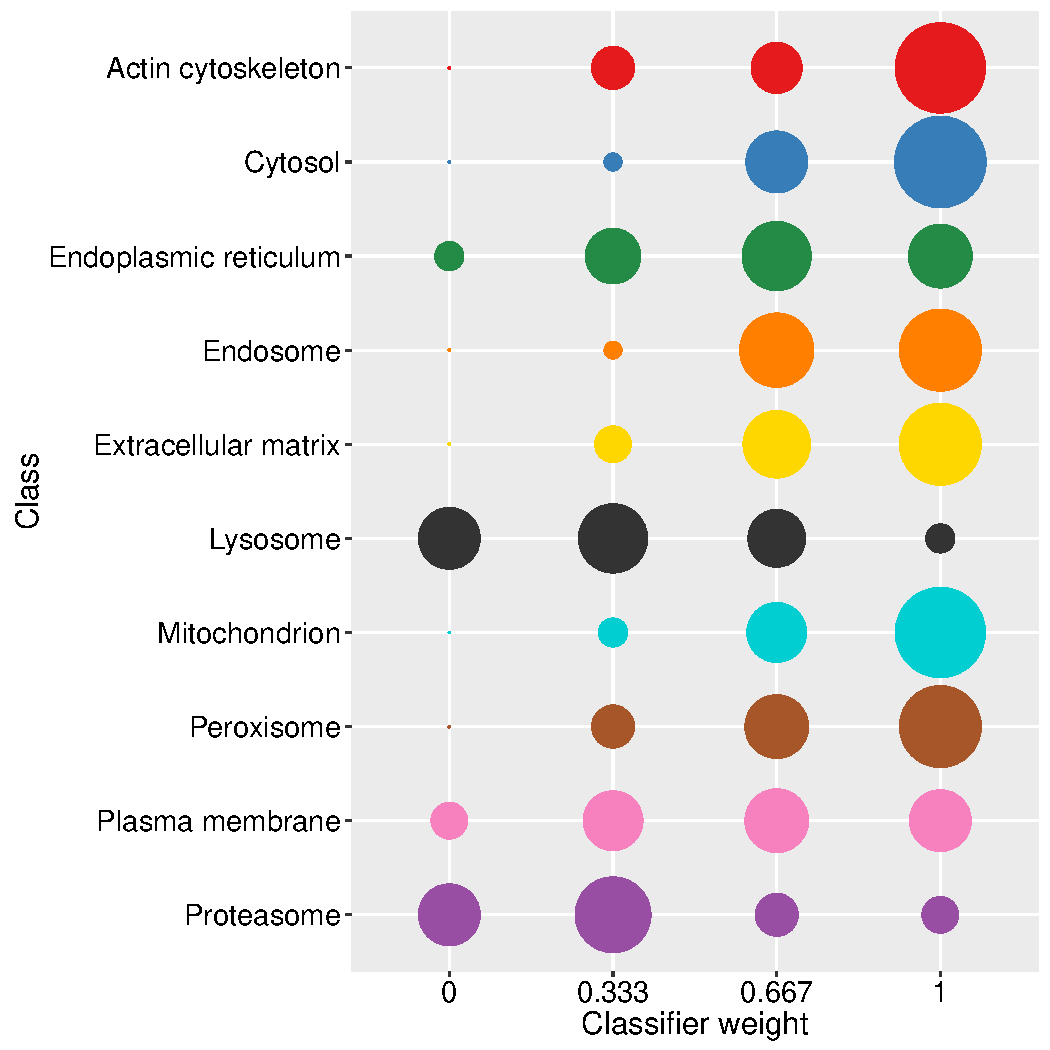
\includegraphics[width=.6\textwidth]{figure/plottl-1} 

\end{knitrout}
\caption{Visualisation of the transfer learning parameter optimisation
  procedure. Each row displays the frequency of observed weights
  (along the columns) for a specific sub-cellular class, with large
  dots representing higher observation frequencies.}
  \label{fig:plottl}
\end{figure}


\subsection*{TL classification} 

Looking at the bubble plot displaying the distribution of best weights
over the 50 runs we find that for many of the subcellular niches a
weight of 1 is most popular (i.e. use only primary hyperLOPIT data in
classification), this is unsuprising as we already know the dataset is
well resolved for these classes. We see that the most popular weights
for the proteasome and lysosome tend to be towards 0, indicating that
these niches are well-resolved in the Gene Ontology. This tells us
that we would benefit from including auxiliary GO information in our
classifier for these subcellular compartments. The plasma membrane
weights are relatively equally spread between using hyperLOPIT and GO
data. Using the \texttt{getParams} function we can return the best
weights and then use this as input for the classification.

One of the benefits of the algorithm is the ability to manually select
weights for each class. In the optimisation above, for time
constraints, we removed the two ribosomal subunits and the two nulcear
compartments, and therefore in the code chunk below when we extract
the best parameters, these subcellular niches are not included. To
include these 4 subcellular niches in the next classification step we
must include them in the parameters. We define a weight of 1 for each
of these niches, as we know they are well resolved in hyperLOPIT. We
then re-order the weights according to \texttt{getMarkerClasses} and
perform the classification using the function
\texttt{knntlClassification}.

\begin{knitrout}
\definecolor{shadecolor}{rgb}{0.969, 0.969, 0.969}\color{fgcolor}\begin{kframe}
\begin{alltt}
\hlcom{## best parameters for the 10 classes}
\hlstd{(bestpar} \hlkwb{<-} \hlkwd{getParams}\hlstd{(tlopt))}
\end{alltt}
\begin{verbatim}
##    Actin cytoskeleton               Cytosol Endoplasmic reticulum 
##             1.0000000             1.0000000             0.6666667 
##              Endosome  Extracellular matrix              Lysosome 
##             1.0000000             1.0000000             0.3333333 
##         Mitochondrion            Peroxisome       Plasma membrane 
##             1.0000000             1.0000000             0.6666667 
##            Proteasome 
##             0.3333333
\end{verbatim}
\begin{alltt}
\hlcom{## add weights for classes not included in the optimisation}
\hlstd{otherweights} \hlkwb{<-} \hlkwd{rep}\hlstd{(}\hlnum{1}\hlstd{,} \hlnum{4}\hlstd{)}
\hlkwd{names}\hlstd{(otherweights)} \hlkwb{<-} \hlkwd{c}\hlstd{(}\hlstr{"40S Ribosome"}\hlstd{,} \hlstr{"60S Ribosome"}\hlstd{,}
                         \hlstr{"Nucleus - Chromatin"}\hlstd{,}
                         \hlstr{"Nucleus - Non-chromatin"}\hlstd{)}
\hlstd{(bestpar} \hlkwb{<-} \hlkwd{c}\hlstd{(bestpar, otherweights))}
\end{alltt}
\begin{verbatim}
##      Actin cytoskeleton                 Cytosol   Endoplasmic reticulum 
##               1.0000000               1.0000000               0.6666667 
##                Endosome    Extracellular matrix                Lysosome 
##               1.0000000               1.0000000               0.3333333 
##           Mitochondrion              Peroxisome         Plasma membrane 
##               1.0000000               1.0000000               0.6666667 
##              Proteasome            40S Ribosome            60S Ribosome 
##               0.3333333               1.0000000               1.0000000 
##     Nucleus - Chromatin Nucleus - Non-chromatin 
##               1.0000000               1.0000000
\end{verbatim}
\begin{alltt}
\hlcom{## re-order classes }
\hlstd{bestpar} \hlkwb{<-} \hlstd{bestpar[}\hlkwd{getMarkerClasses}\hlstd{(hl)]}

\hlcom{## Do the classification}
\hlstd{hl} \hlkwb{<-} \hlkwd{knntlClassification}\hlstd{(hl, gocc,} \hlkwc{bestTheta} \hlstd{= bestpar,} \hlkwc{k} \hlstd{=} \hlkwd{c}\hlstd{(}\hlnum{3}\hlstd{,} \hlnum{3}\hlstd{))}
\end{alltt}
\end{kframe}
\end{knitrout}

The results from the classification results and associated scores are
appended to the \texttt{fData} slot and named \texttt{knntl} and
\texttt{knntl.scores} respectively. Results can be visualised using
\texttt{plot2D}, scores assessed and cutoffs calculated using the
\texttt{classify} app in \texttt{pRolocVis}, predictions obtained
using \texttt{getPredictions} in the same way as demonstrated above
for the SVM classifier.

\section*{Unsupervised machine learning}

In \texttt{pRoloc} there is functionality for unsupervsied machine
learning methods. In unsupervised learning, the training data consists
of a set of input vectors e.g. protein profiles, ignoring the
information about the class label e.g. localisation, other than for
annotation purposes. The main goal in unsupervised learning is to
uncover groups of similar features within the data, termed
clustering. Ordination methods such as principal components analysis
(PCA) also fall into the category of unsupervised learning methods,
where the data can be projected from a high-dimensional space down to
two or three dimensions for the purpose of visualisation.

As described and demonstrated already above, PCA is a valuable and
powerful method for data visualisation and quality control. Another
application uses hierarchical clustering to summarise the relation
between marker proteins using he \texttt{mrkHClust} function, where
the euclidean distance bewteen average class-specific profiles is used
to produce a dendrogramme describing a simple relationship between the
sub-cellular classes (Figure~\ref{fig:mrkHclust}). The
\texttt{mrkHClust} uses the same defaults as all other function, using
the \texttt{markers} feature variable to define marker proteins. In
the code chunk, we adapt the figure margins to fully display the class
names.

\begin{figure}[!ht]
  \centering
\begin{knitrout}
\definecolor{shadecolor}{rgb}{0.969, 0.969, 0.969}\color{fgcolor}\begin{kframe}
\begin{alltt}
\hlkwd{par}\hlstd{(}\hlkwc{mar} \hlstd{=} \hlkwd{c}\hlstd{(}\hlnum{15}\hlstd{,} \hlnum{4}\hlstd{,} \hlnum{1}\hlstd{,} \hlnum{0}\hlstd{))}
\hlkwd{mrkHClust}\hlstd{(hl)}
\end{alltt}
\end{kframe}
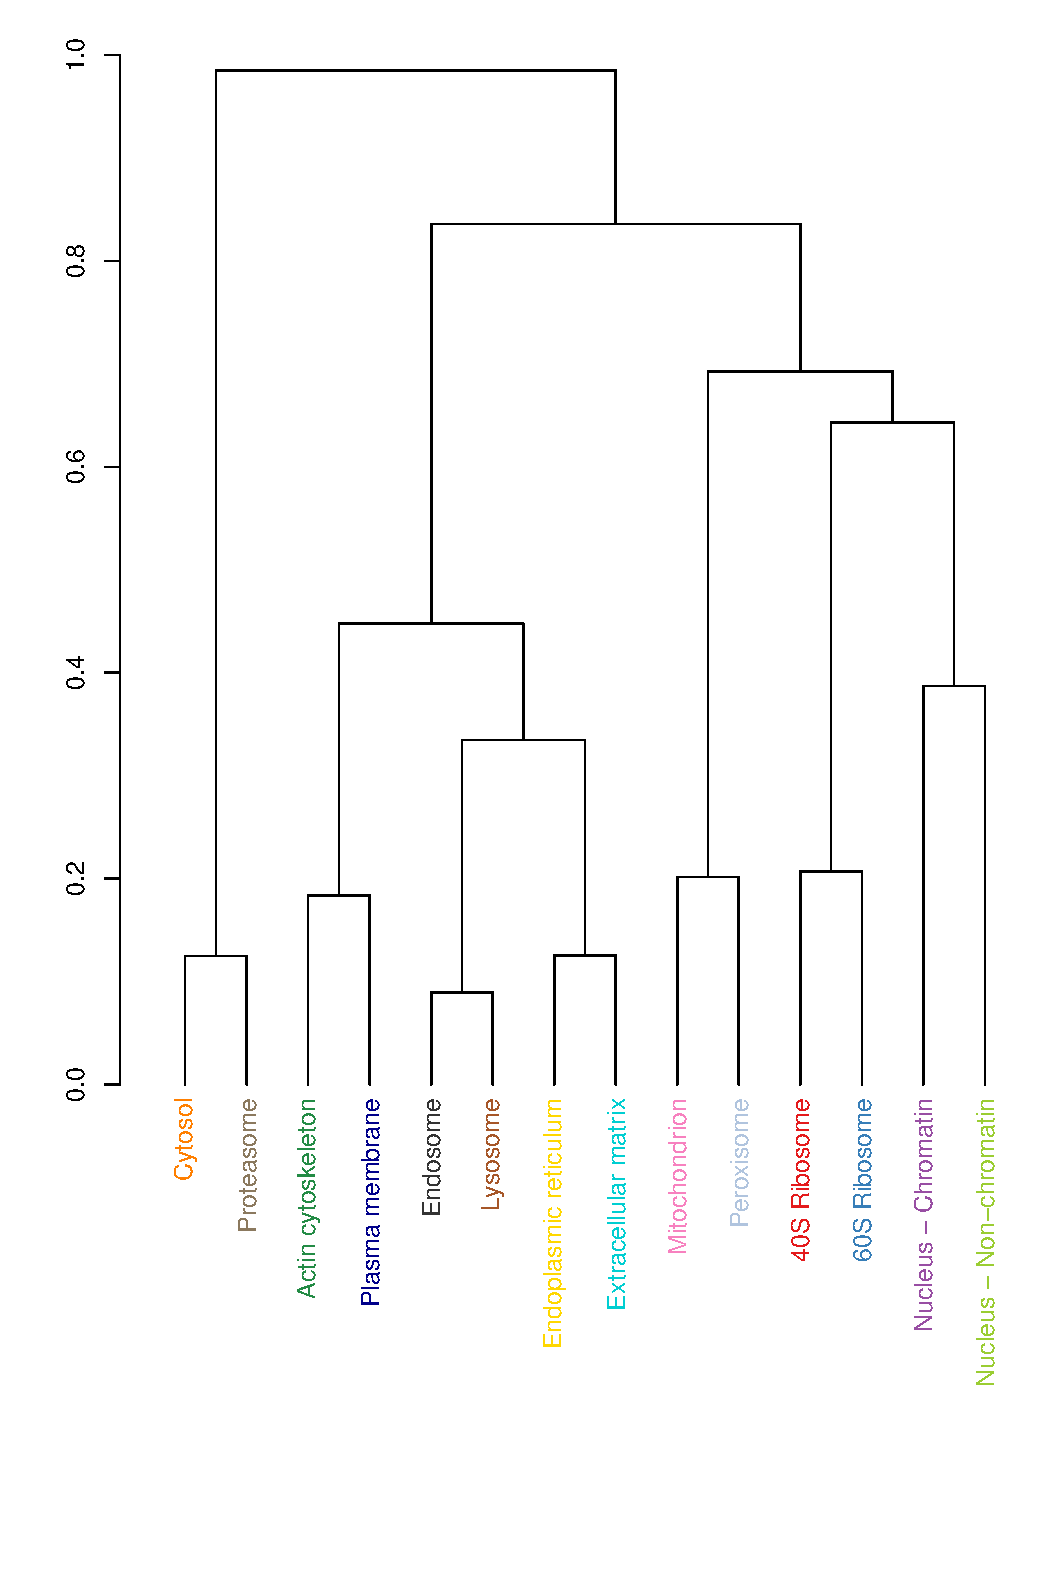
\includegraphics[width=.5\textwidth,angle=-90]{figure/hclust-1} 

\end{knitrout}
  \caption{Hierarchical clustering of the average marker profiles summarising the relation between organelles profiles.}
  \label{fig:mrkHclust}
\end{figure}

We generally find supervised learning more suited to the task of
protein localisation prediction in which we use high-quality curated
marker proteins to build a classifier, instead of using an entirely
unsupervised approach to look for clusters and then look for
enrichment of organelles and complexes. In the latter we do not make
good use of valuable prior knowledge, and in our experience
unsupervised clustering can be extremely difficult due poor estimates
of the number of clusters that may appear in the data.

\section*{Writing and exporting data}

An \texttt{MSnSet} can be exported from R using the
\texttt{write.exprs} function.  This function writes the expression
values to a text-based spreadsheet. The \texttt{fcol} argument can be
used to specify which \texttt{featureData} columns (as column names,
column number or \texttt{logical}) to append to the right of the
expression matrix.

In the below code chunk we write the \texttt{hl} object to a csv
file. The \texttt{file} argument is used to specify the file path, the
\texttt{sep} argument specifies the field separator string, here we
use a comma, finally as we want to write all the information in the
\texttt{featureData} to the file, as well as the expression data, we
specify \texttt{fvarLabels(hl)}, that returns all feature variable
names, and write the resulting data to the file \texttt{"hl.csv"}.

\begin{knitrout}
\definecolor{shadecolor}{rgb}{0.969, 0.969, 0.969}\color{fgcolor}\begin{kframe}
\begin{alltt}
\hlkwd{write.exprs}\hlstd{(hl,} \hlkwc{file} \hlstd{=} \hlstr{"hl.csv"}\hlstd{,} \hlkwc{sep} \hlstd{=} \hlstr{","}\hlstd{,} \hlkwc{fcol} \hlstd{=} \hlkwd{fvarLabels}\hlstd{(hl))}
\end{alltt}
\end{kframe}
\end{knitrout}

Exporting to a spreadsheet however looses a lot of important
information, such as the processing data, and the sample metadata in
the \textit{phenoData} slot. Other objects, such a parameters from the
machine learning optimisation, cannot be represented as tabular
data. To directly serialise R objects to disk, on can use the standard
\texttt{save} function, and later reload the object using
\texttt{save}. For example, to save and then re-load the parameters
from the SVM optimisation,

\begin{knitrout}
\definecolor{shadecolor}{rgb}{0.969, 0.969, 0.969}\color{fgcolor}\begin{kframe}
\begin{alltt}
\hlcom{## To save the parameters as an R object}
\hlkwd{save}\hlstd{(params,} \hlkwc{file} \hlstd{=} \hlstr{"svmparams.rda"}\hlstd{)}

\hlcom{## To re-load after saving}
\hlkwd{load}\hlstd{(}\hlkwc{file} \hlstd{=} \hlstr{"svmparams.rda"}\hlstd{)}
\end{alltt}
\end{kframe}
\end{knitrout}

\section*{Session information}

The function \texttt{sessionInfo} provides a summary of all packages
and versions used to generate this document. This enables us to record
the exact state of our session that lead to these results. Conversely,
if the script stops working or if it returns different results, we are
in a position to re-generate the original results using the adequate
software versions and retrace changes in the software that lead to
failure and/or different results.

\begin{knitrout}
\definecolor{shadecolor}{rgb}{0.969, 0.969, 0.969}\color{fgcolor}\begin{kframe}
\begin{alltt}
\hlkwd{sessionInfo}\hlstd{()}
\end{alltt}
\begin{verbatim}
## R version 3.3.2 Patched (2016-11-01 r71616)
## Platform: x86_64-pc-linux-gnu (64-bit)
## Running under: Ubuntu 14.04.5 LTS
## 
## locale:
##  [1] LC_CTYPE=en_GB.UTF-8       LC_NUMERIC=C              
##  [3] LC_TIME=en_GB.UTF-8        LC_COLLATE=en_GB.UTF-8    
##  [5] LC_MONETARY=en_GB.UTF-8    LC_MESSAGES=en_GB.UTF-8   
##  [7] LC_PAPER=en_GB.UTF-8       LC_NAME=C                 
##  [9] LC_ADDRESS=C               LC_TELEPHONE=C            
## [11] LC_MEASUREMENT=en_GB.UTF-8 LC_IDENTIFICATION=C       
## 
## attached base packages:
## [1] stats4    parallel  methods   stats     graphics  grDevices utils    
## [8] datasets  base     
## 
## other attached packages:
##  [1] pRolocdata_1.12.0    pRoloc_1.15.5        MLInterfaces_1.54.0 
##  [4] cluster_2.0.5        annotate_1.52.0      XML_3.98-1.5        
##  [7] AnnotationDbi_1.36.0 IRanges_2.8.1        S4Vectors_0.12.1    
## [10] MSnbase_2.1.4        ProtGenerics_1.6.0   BiocParallel_1.8.1  
## [13] mzR_2.8.0            Rcpp_0.12.8          Biobase_2.34.0      
## [16] BiocGenerics_0.20.0  gridExtra_2.2.1      xtable_1.8-2        
## [19] BiocStyle_2.2.1      knitr_1.15.1        
## 
## loaded via a namespace (and not attached):
##   [1] minqa_1.2.4           colorspace_1.3-1      hwriter_1.3.2        
##   [4] class_7.3-14          modeltools_0.2-21     mclust_5.2           
##   [7] pls_2.5-0             base64enc_0.1-3       proxy_0.4-16         
##  [10] hexbin_1.27.1         MatrixModels_0.4-1    affyio_1.44.0        
##  [13] flexmix_2.3-13        mvtnorm_1.0-5         codetools_0.2-15     
##  [16] splines_3.3.2         doParallel_1.0.10     impute_1.48.0        
##  [19] robustbase_0.92-6     jsonlite_1.1          nloptr_1.0.4         
##  [22] caret_6.0-73          pbkrtest_0.4-6        rda_1.0.2-2          
##  [25] kernlab_0.9-25        vsn_3.42.3            sfsmisc_1.1-0        
##  [28] shiny_0.14.2          sampling_2.7          assertthat_0.1       
##  [31] Matrix_1.2-7.1        lazyeval_0.2.0        limma_3.30.6         
##  [34] htmltools_0.3.5       quantreg_5.29         tools_3.3.2          
##  [37] ggvis_0.4.3           gtable_0.2.0          affy_1.52.0          
##  [40] reshape2_1.4.2        dplyr_0.5.0           MALDIquant_1.15      
##  [43] trimcluster_0.1-2     gdata_2.17.0          preprocessCore_1.36.0
##  [46] nlme_3.1-128          iterators_1.0.8       fpc_2.1-10           
##  [49] stringr_1.1.0         lme4_1.1-12           lpSolve_5.6.13       
##  [52] mime_0.5              gtools_3.5.0          dendextend_1.3.0     
##  [55] DEoptimR_1.0-8        zlibbioc_1.20.0       MASS_7.3-45          
##  [58] scales_0.4.1          BiocInstaller_1.24.0  pcaMethods_1.66.0    
##  [61] SparseM_1.74          RColorBrewer_1.1-2    memoise_1.0.0        
##  [64] ggplot2_2.2.0         biomaRt_2.30.0        rpart_4.1-10         
##  [67] stringi_1.1.2         RSQLite_1.1           highr_0.6            
##  [70] genefilter_1.56.0     randomForest_4.6-12   foreach_1.4.3        
##  [73] e1071_1.6-7           prabclus_2.2-6        bitops_1.0-6         
##  [76] mzID_1.12.0           evaluate_0.10         lattice_0.20-34      
##  [79] htmlwidgets_0.8       gbm_2.1.1             plyr_1.8.4           
##  [82] magrittr_1.5          R6_2.2.0              DBI_0.5-1            
##  [85] whisker_0.3-2         mgcv_1.8-16           survival_2.40-1      
##  [88] RCurl_1.95-4.8        nnet_7.3-12           tibble_1.2           
##  [91] msdata_0.14.0         car_2.1-3             mlbench_2.1-1        
##  [94] grid_3.3.2            FNN_1.1               ModelMetrics_1.1.0   
##  [97] threejs_0.2.2         digest_0.6.10         diptest_0.75-7       
## [100] httpuv_1.3.3          munsell_0.4.3
\end{verbatim}
\end{kframe}
\end{knitrout}

We also recommend that users regularly update the packages as well as
the R itself. This can be done with the \texttt{biocLite} function.

\begin{knitrout}
\definecolor{shadecolor}{rgb}{0.969, 0.969, 0.969}\color{fgcolor}\begin{kframe}
\begin{alltt}
\hlkwd{library}\hlstd{(}\hlstr{"BiocInstaller"}\hlstd{)}
\hlkwd{biocLite}\hlstd{()}
\end{alltt}
\end{kframe}
\end{knitrout}

It is always important to include session information details along
with a \href{http://adv-r.had.co.nz/Reproducibility.html}{short
  reproducible example} highlighting the problem or
\href{https://support.bioconductor.org/}{question} at hand. 

The source of this document, including the code necessary to reproduce
the analyses and figures is available in a public manuscript
repository on GitHub~\cite{ghrepo}.

\bigskip

\subsection*{Author contributions}

LMB and LG developed the software presented in this workflow. All
authors wrote and approved the manuscript.

\subsection*{Competing interests}

The authors declare that they have no competing interest. 

\subsection*{Grant information}

LMB is supported by a Wellcome Trust Technology Development Grant
(grant number 108467/Z/15/Z). LG is supported by the BBSRC Strategic
Longer and Larger grant (Award BB/L002817/1).


\subsection*{Acknowledgements}

The authors would like to thank Dr. Stuart Rankin from the High
Performance Computing Service for his support. Part of this work was
performed using the Darwin Supercomputer of the University of
Cambridge High Performance Computing Service, provided by Dell
Inc. using Strategic Research Infrastructure Funding from the Higher
Education Funding Council for England and funding from the Science and
Technology Facilities Council.


\end{document}